\chapter[$\Htautau$ analysis strategy][$\Htautau$ analysis strategy]{$\Htautau$ analysis strategy}
\label{chap:strategy}

\begin{quote}
The strategy of the $\Htautau$ strategy is described.
\end{quote}

\section{Introduction}
\label{sec:strategy-introduction}

\begin{figure}[tp]
  \centering
  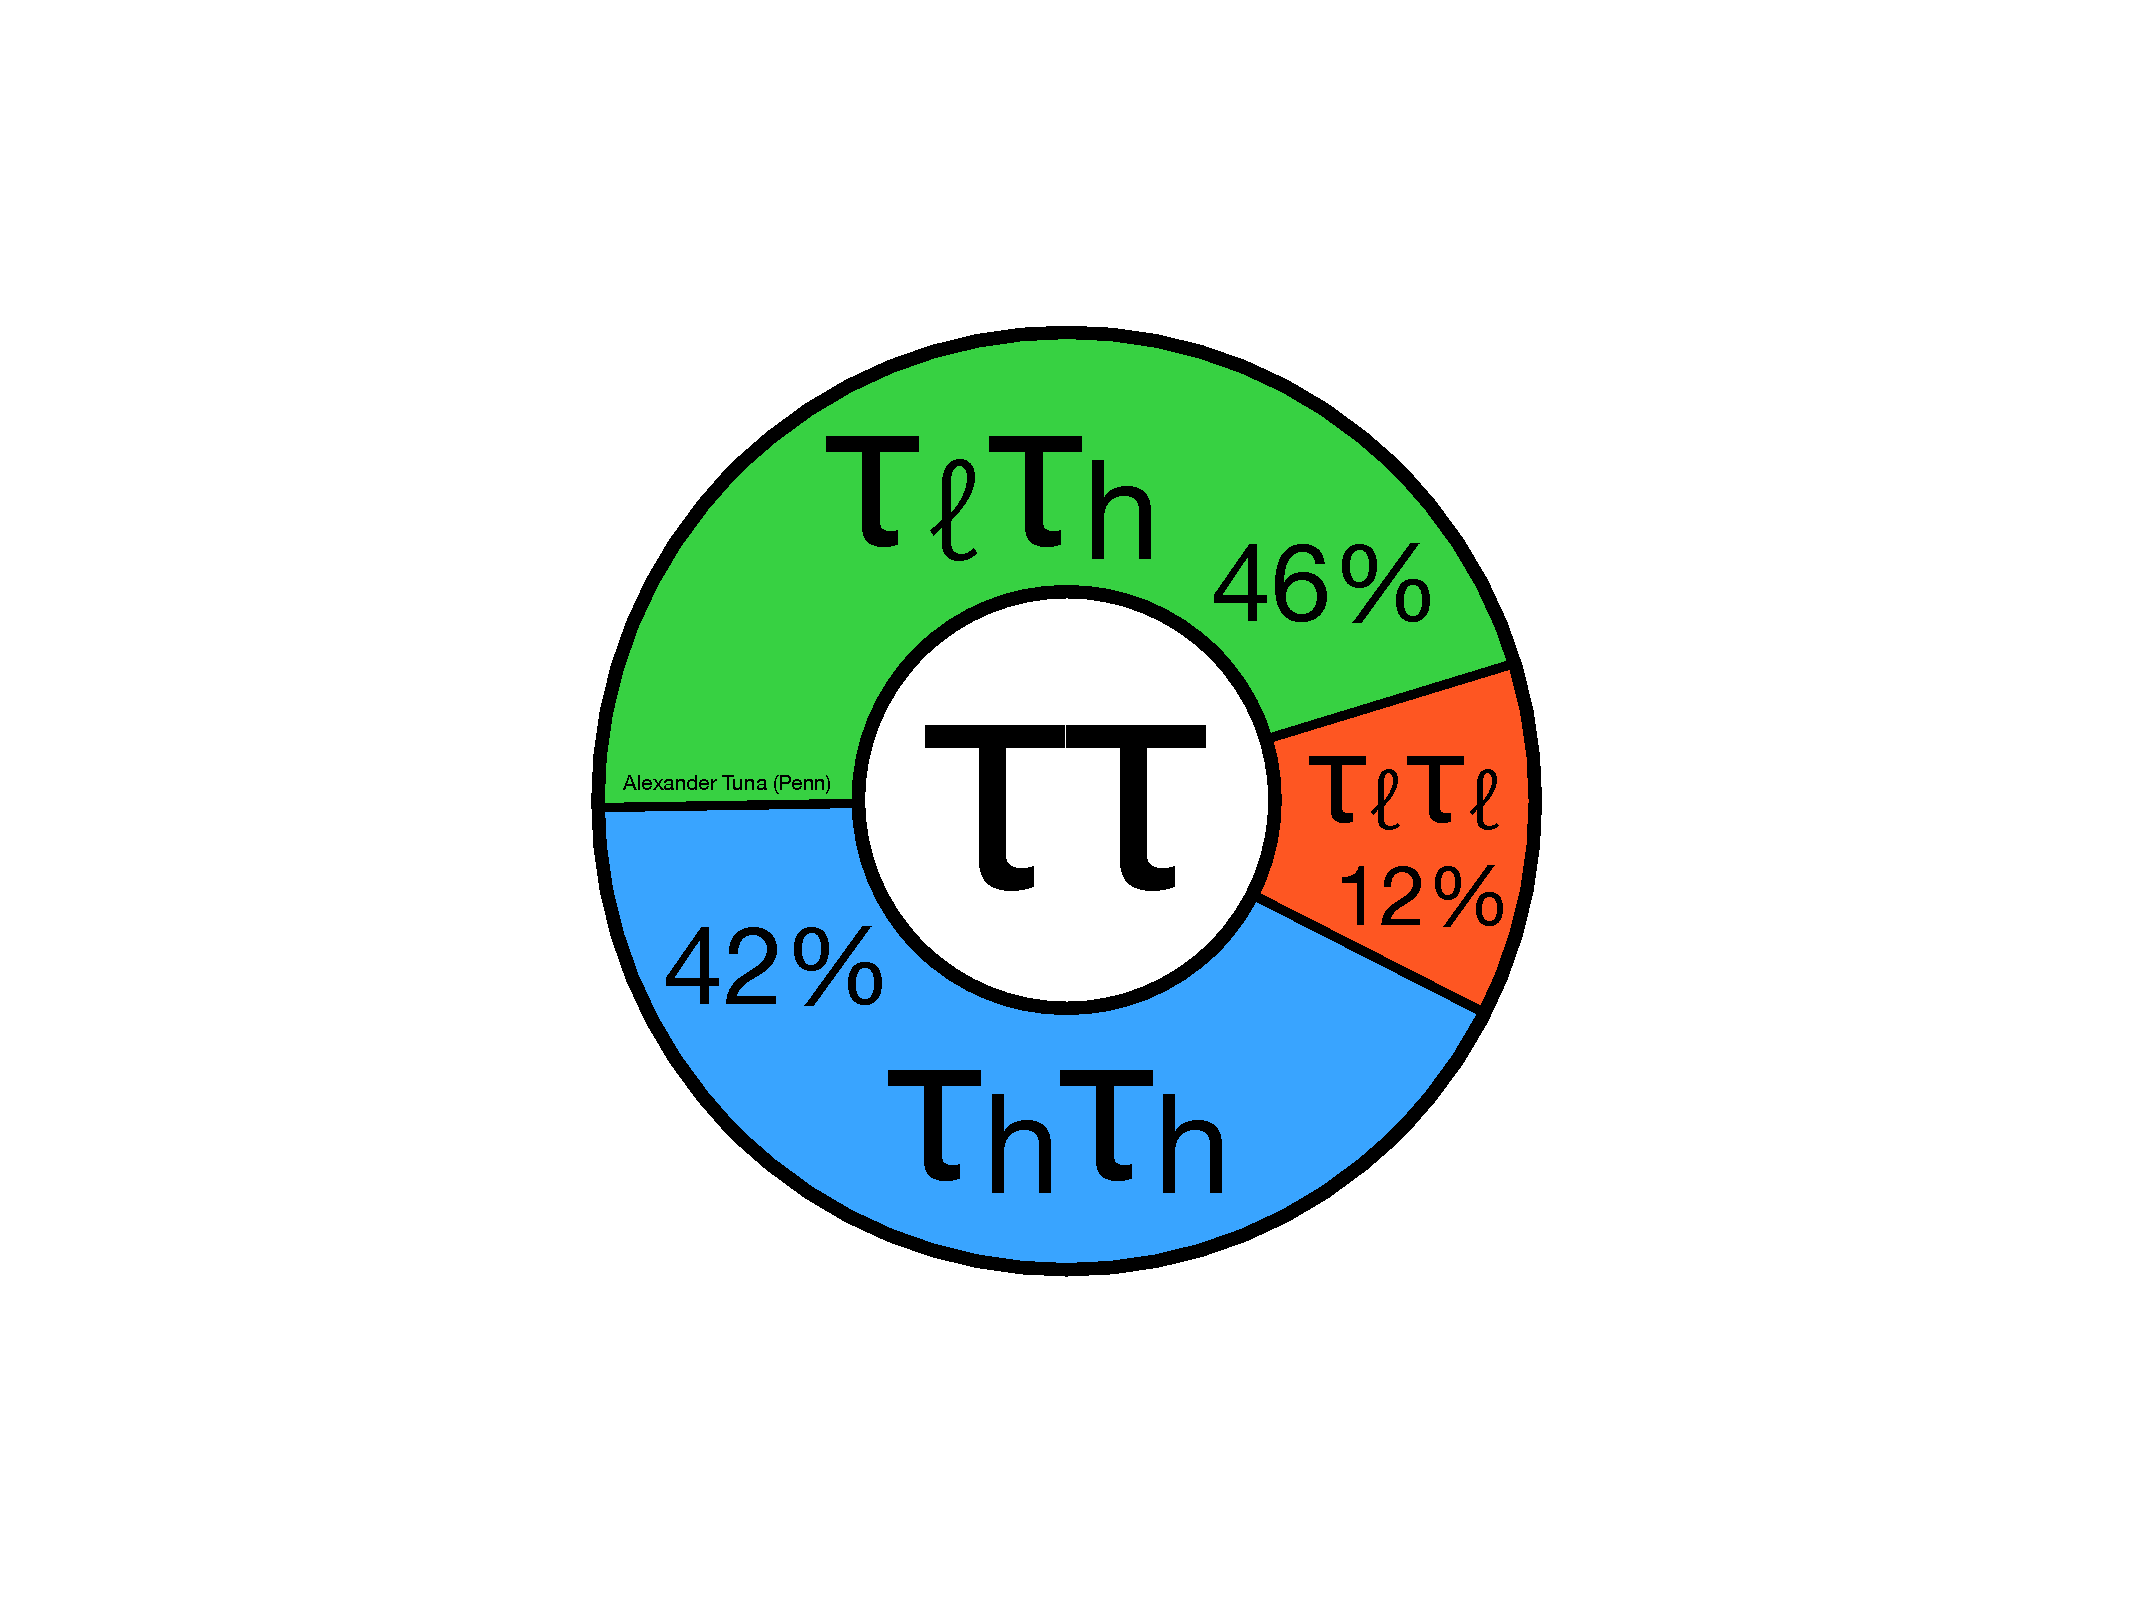
\includegraphics[width=0.48\textwidth]{figures/piecharts/tautaudecay}
  \caption{Variables.}
  \label{fig:strategy-decaypie}
\end{figure}

\section{Physics objects}
\label{sec:strategy-objects}

\begin{figure}[tp]
  \centering
  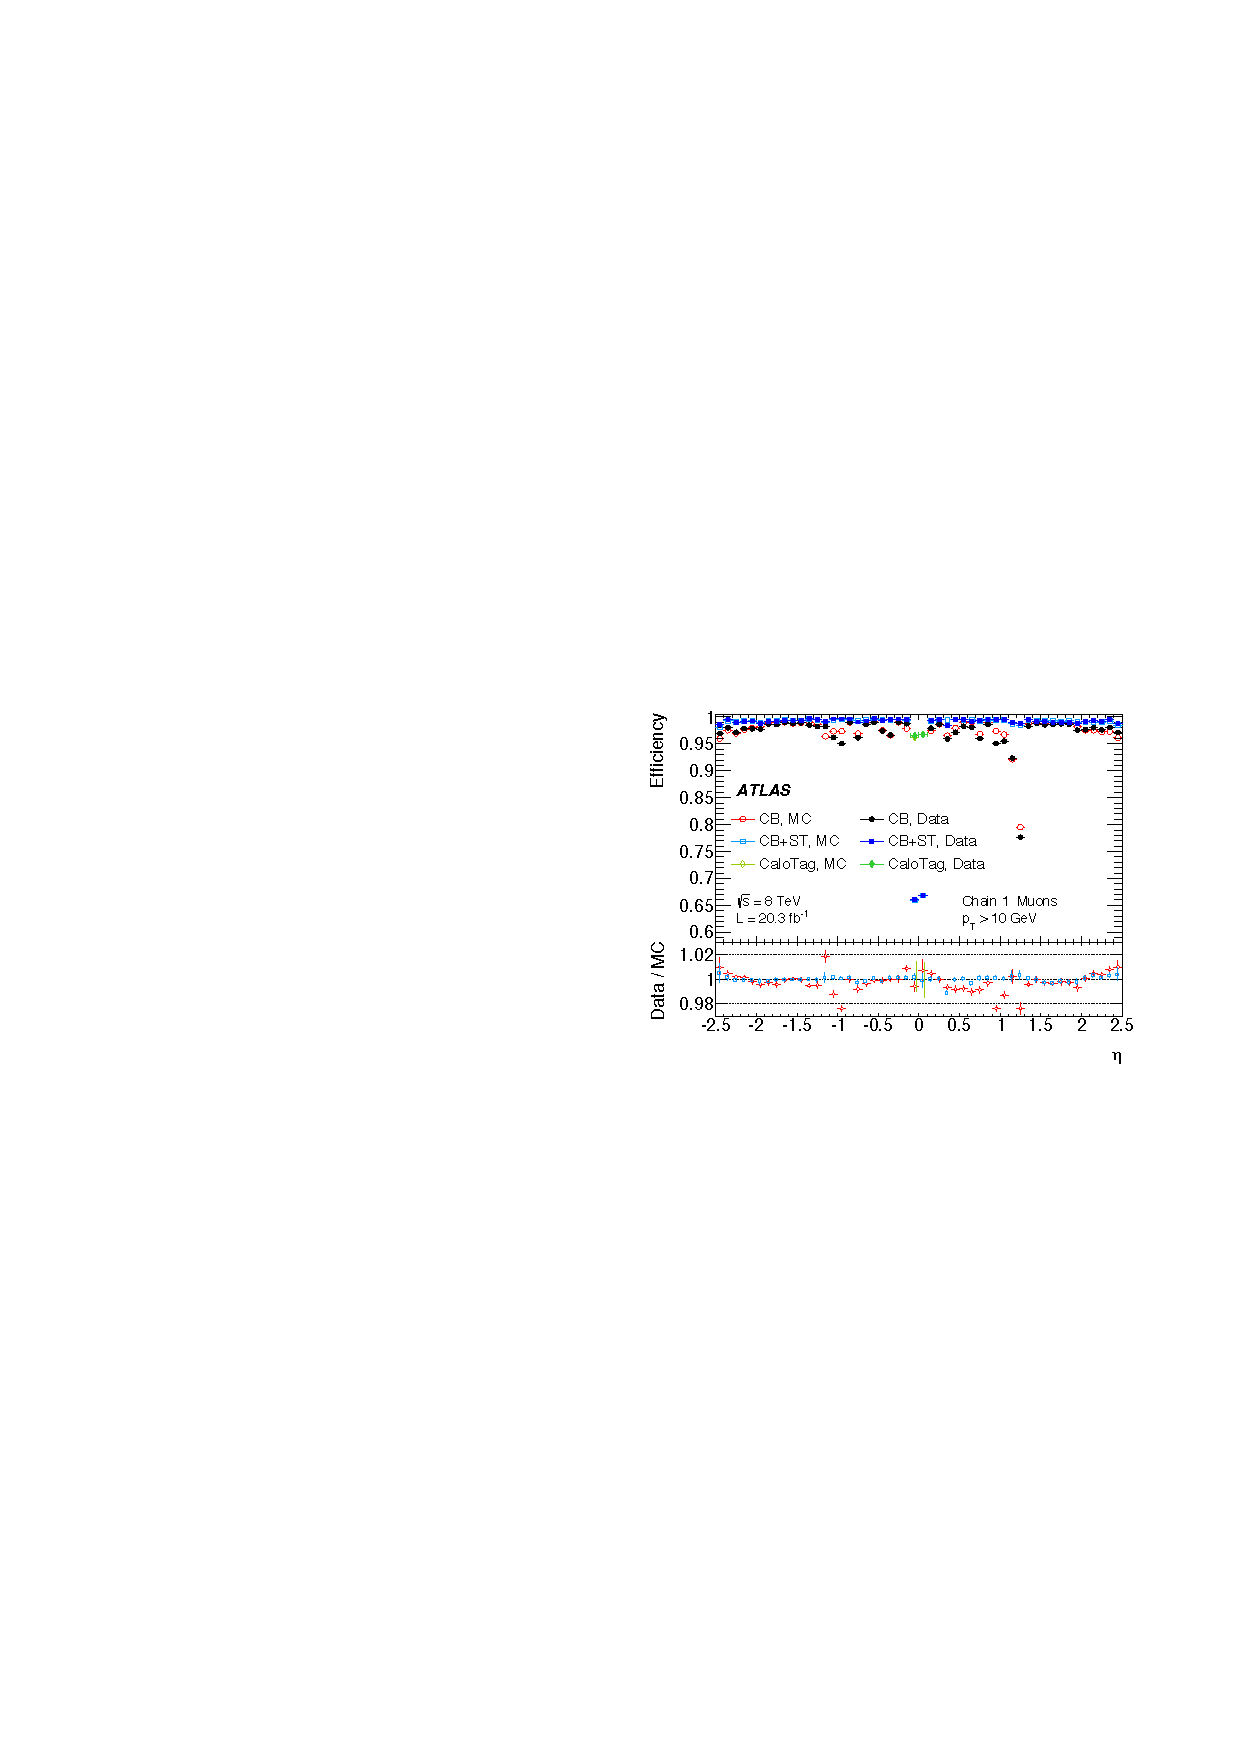
\includegraphics[width=0.48\textwidth]{figures/performance/muon-efficiency}
  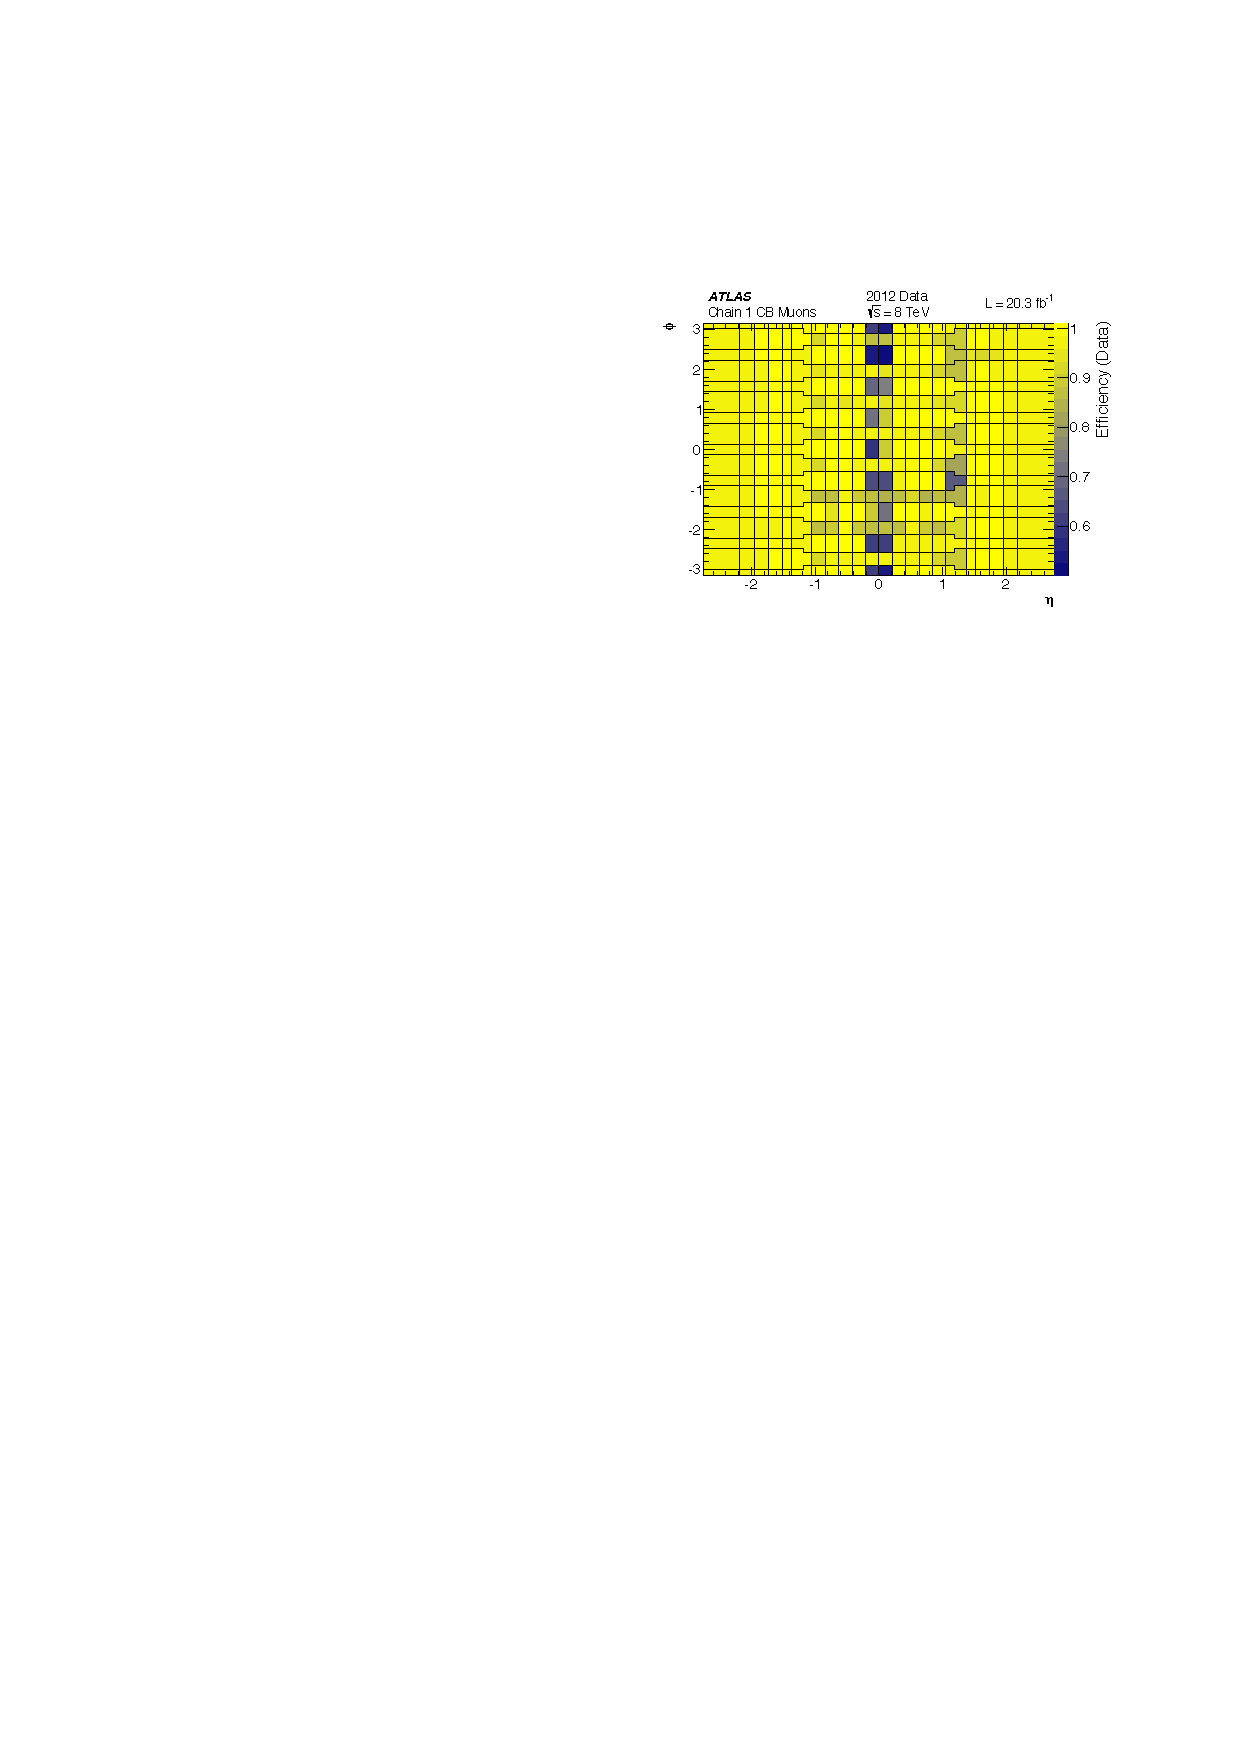
\includegraphics[width=0.48\textwidth]{figures/performance/muon-efficiency-etaphi}
  \caption{Variables.}
  \label{fig:strategy-objects-muon-efficiency}
\end{figure}

\begin{figure}[tp]
  \centering
  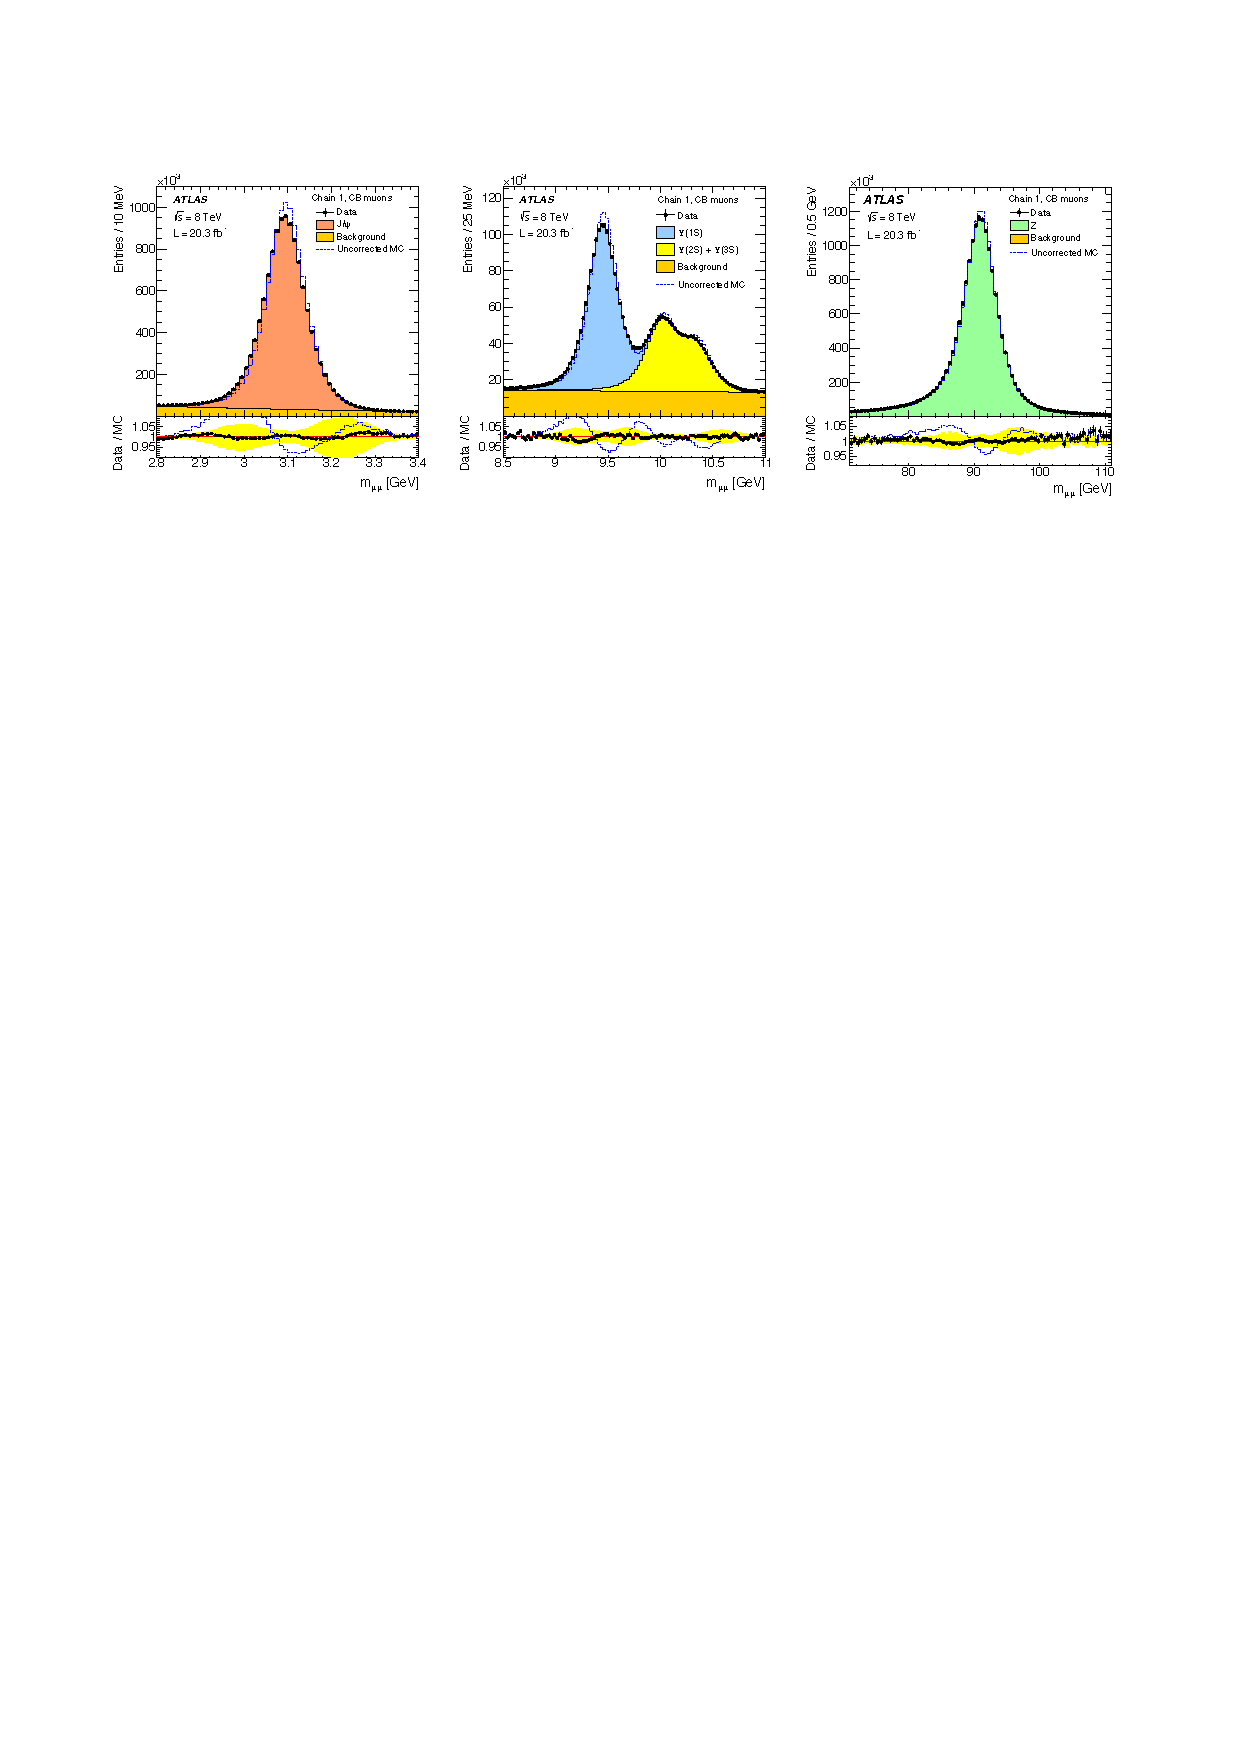
\includegraphics[width=0.90\textwidth]{figures/performance/muon-energyscale}
  \caption{Variables.}
  \label{fig:strategy-objects-muon-energyscale}
\end{figure}

\begin{figure}[tp]
  \centering
  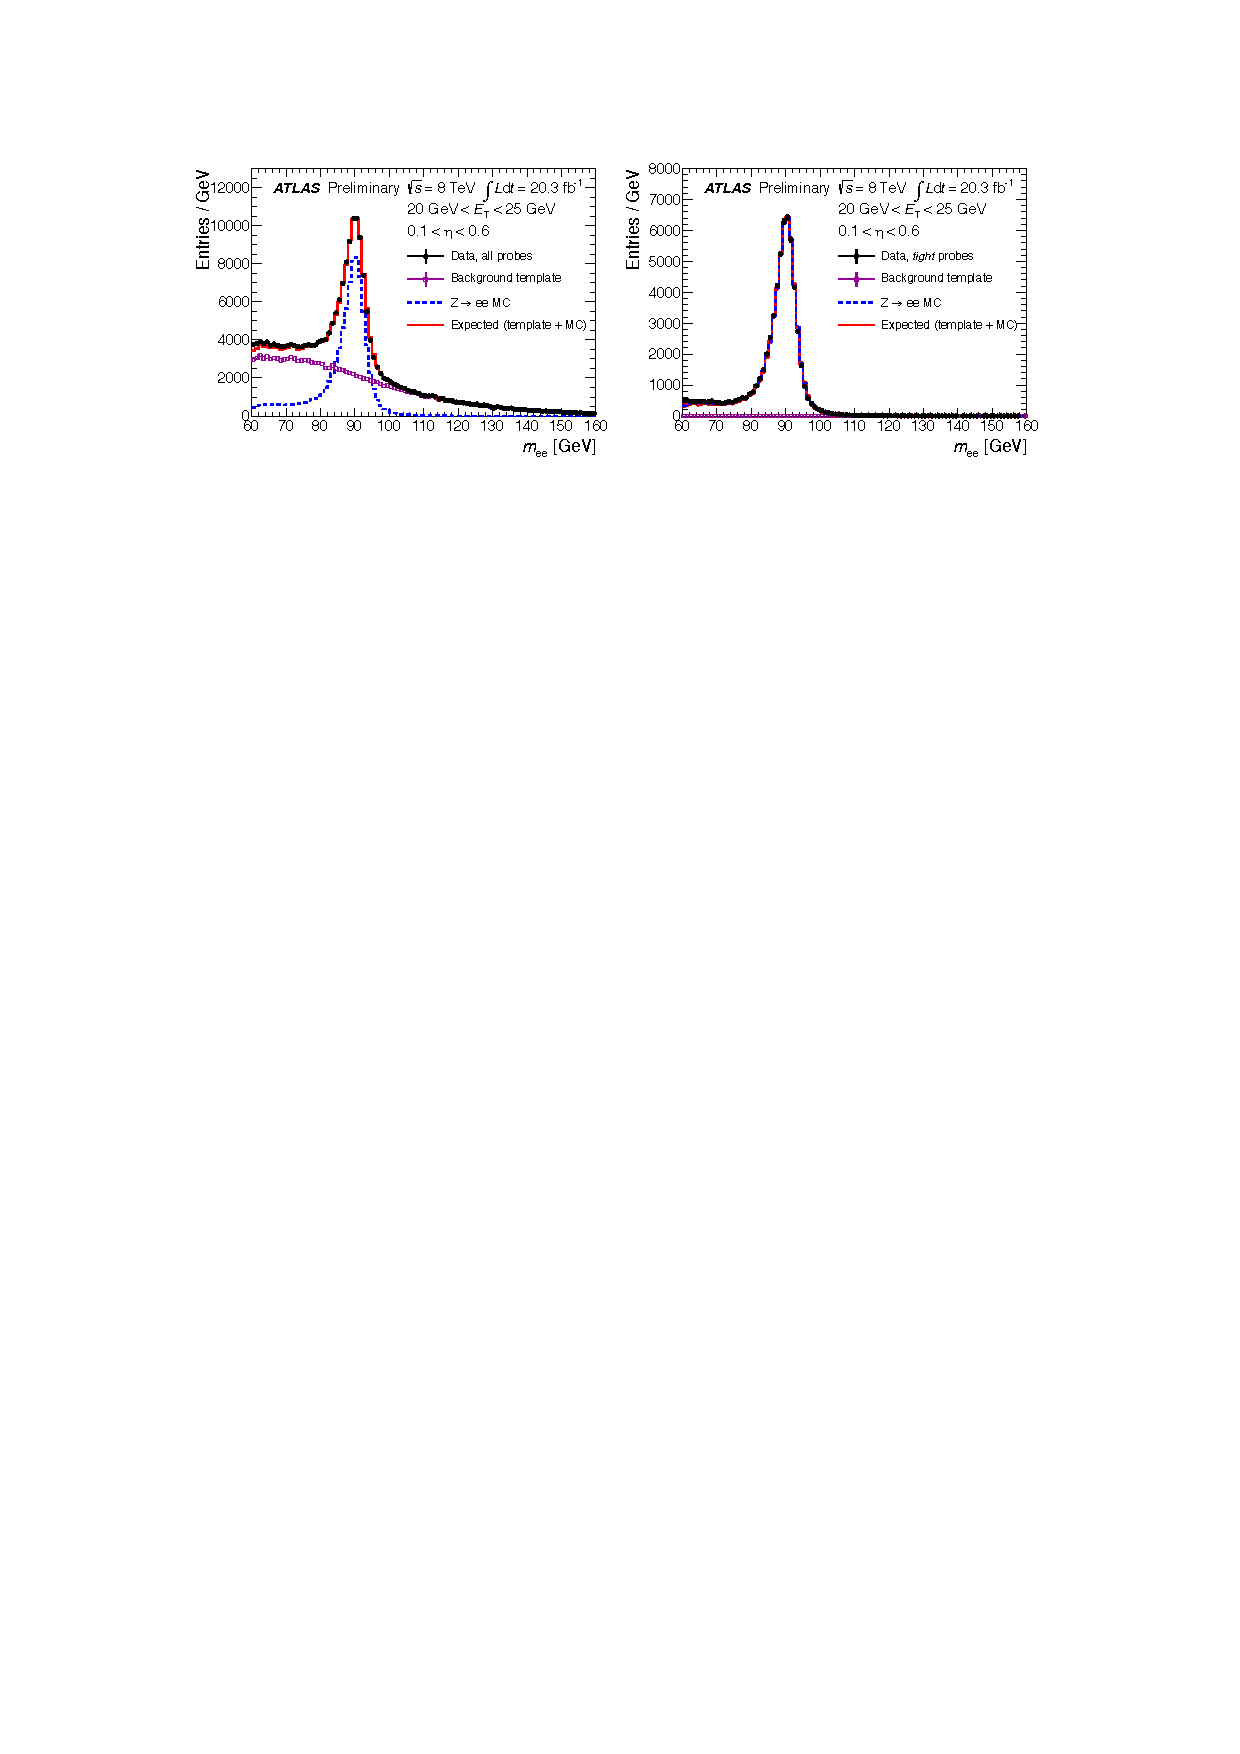
\includegraphics[width=0.90\textwidth]{figures/performance/electron-ZeeTP}
  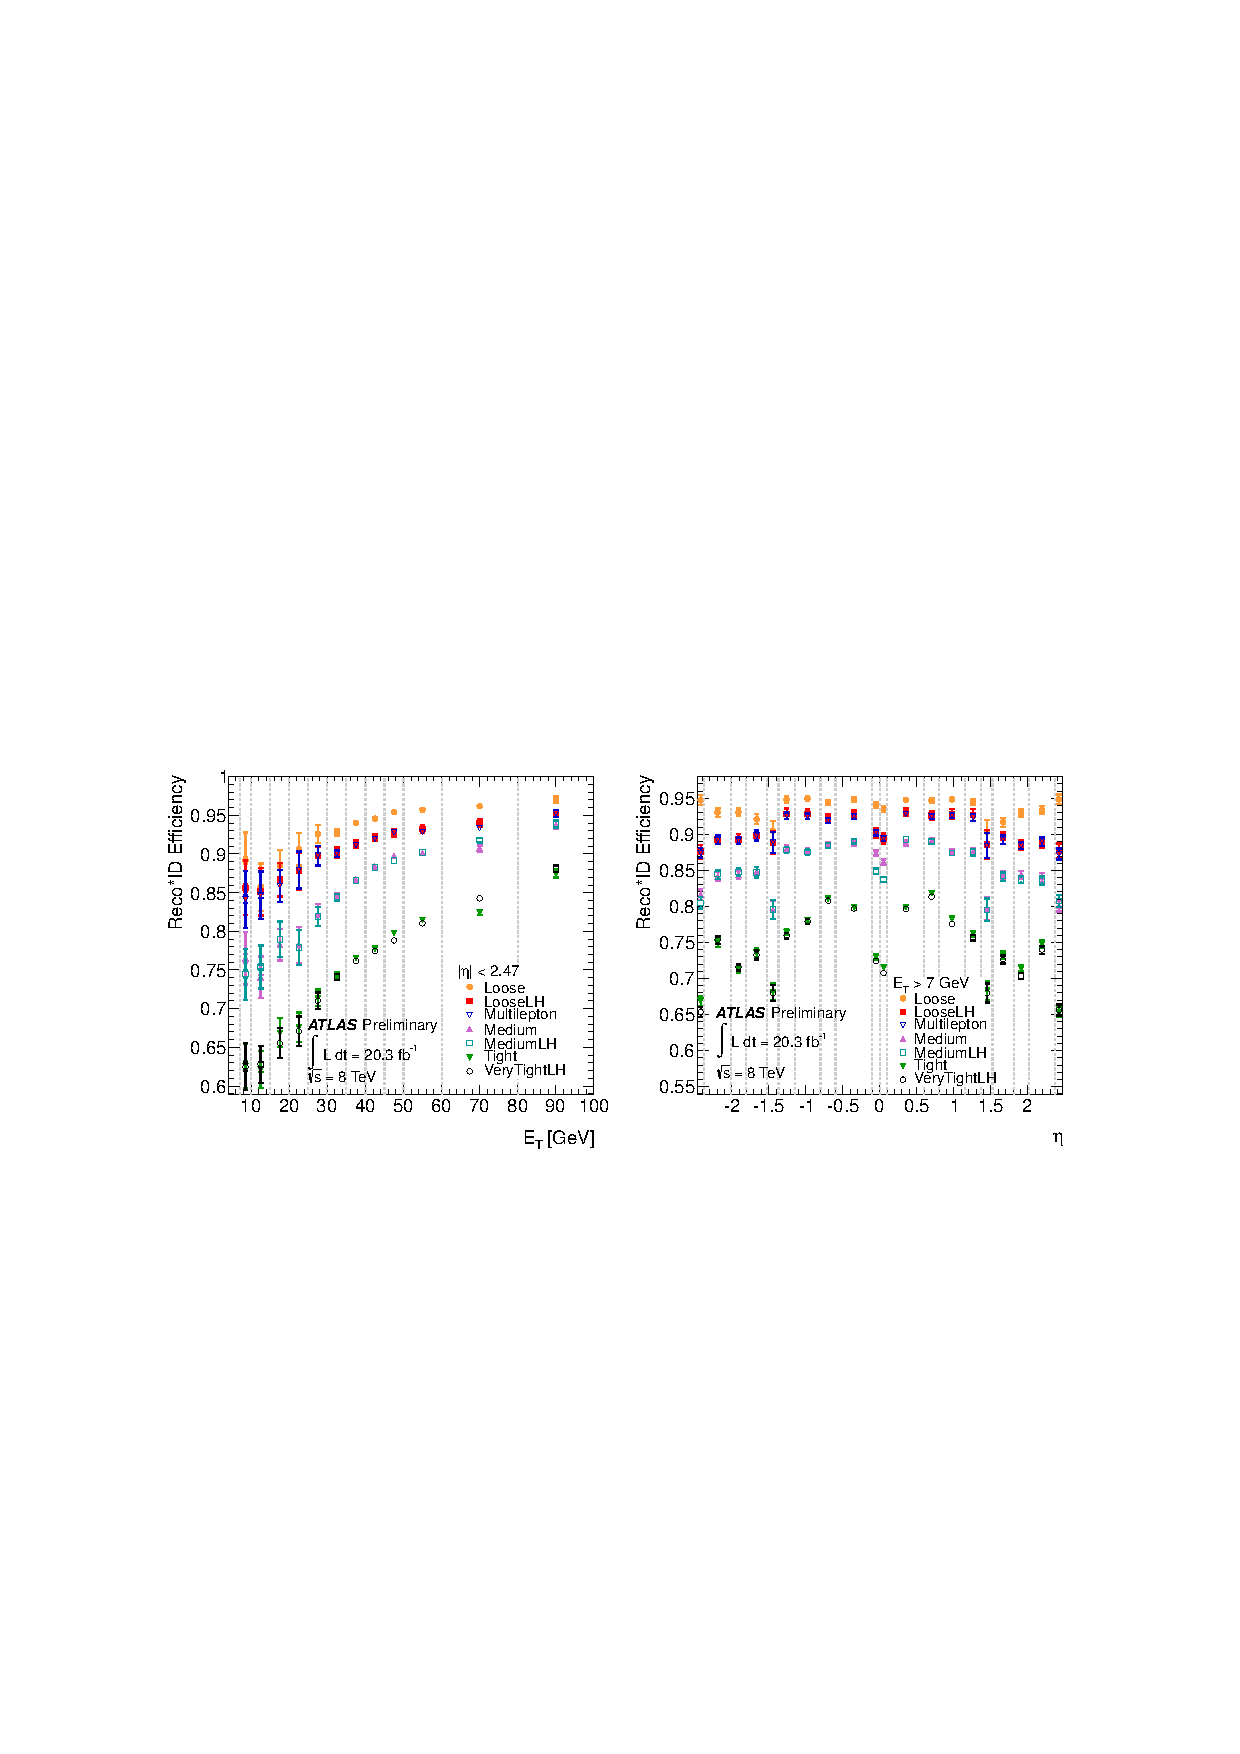
\includegraphics[width=0.90\textwidth]{figures/performance/electron-recoIDefficiecy}
  \caption{Variables.}
  \label{fig:strategy-objects-electron}
\end{figure}

\begin{figure}[tp]
  \centering
  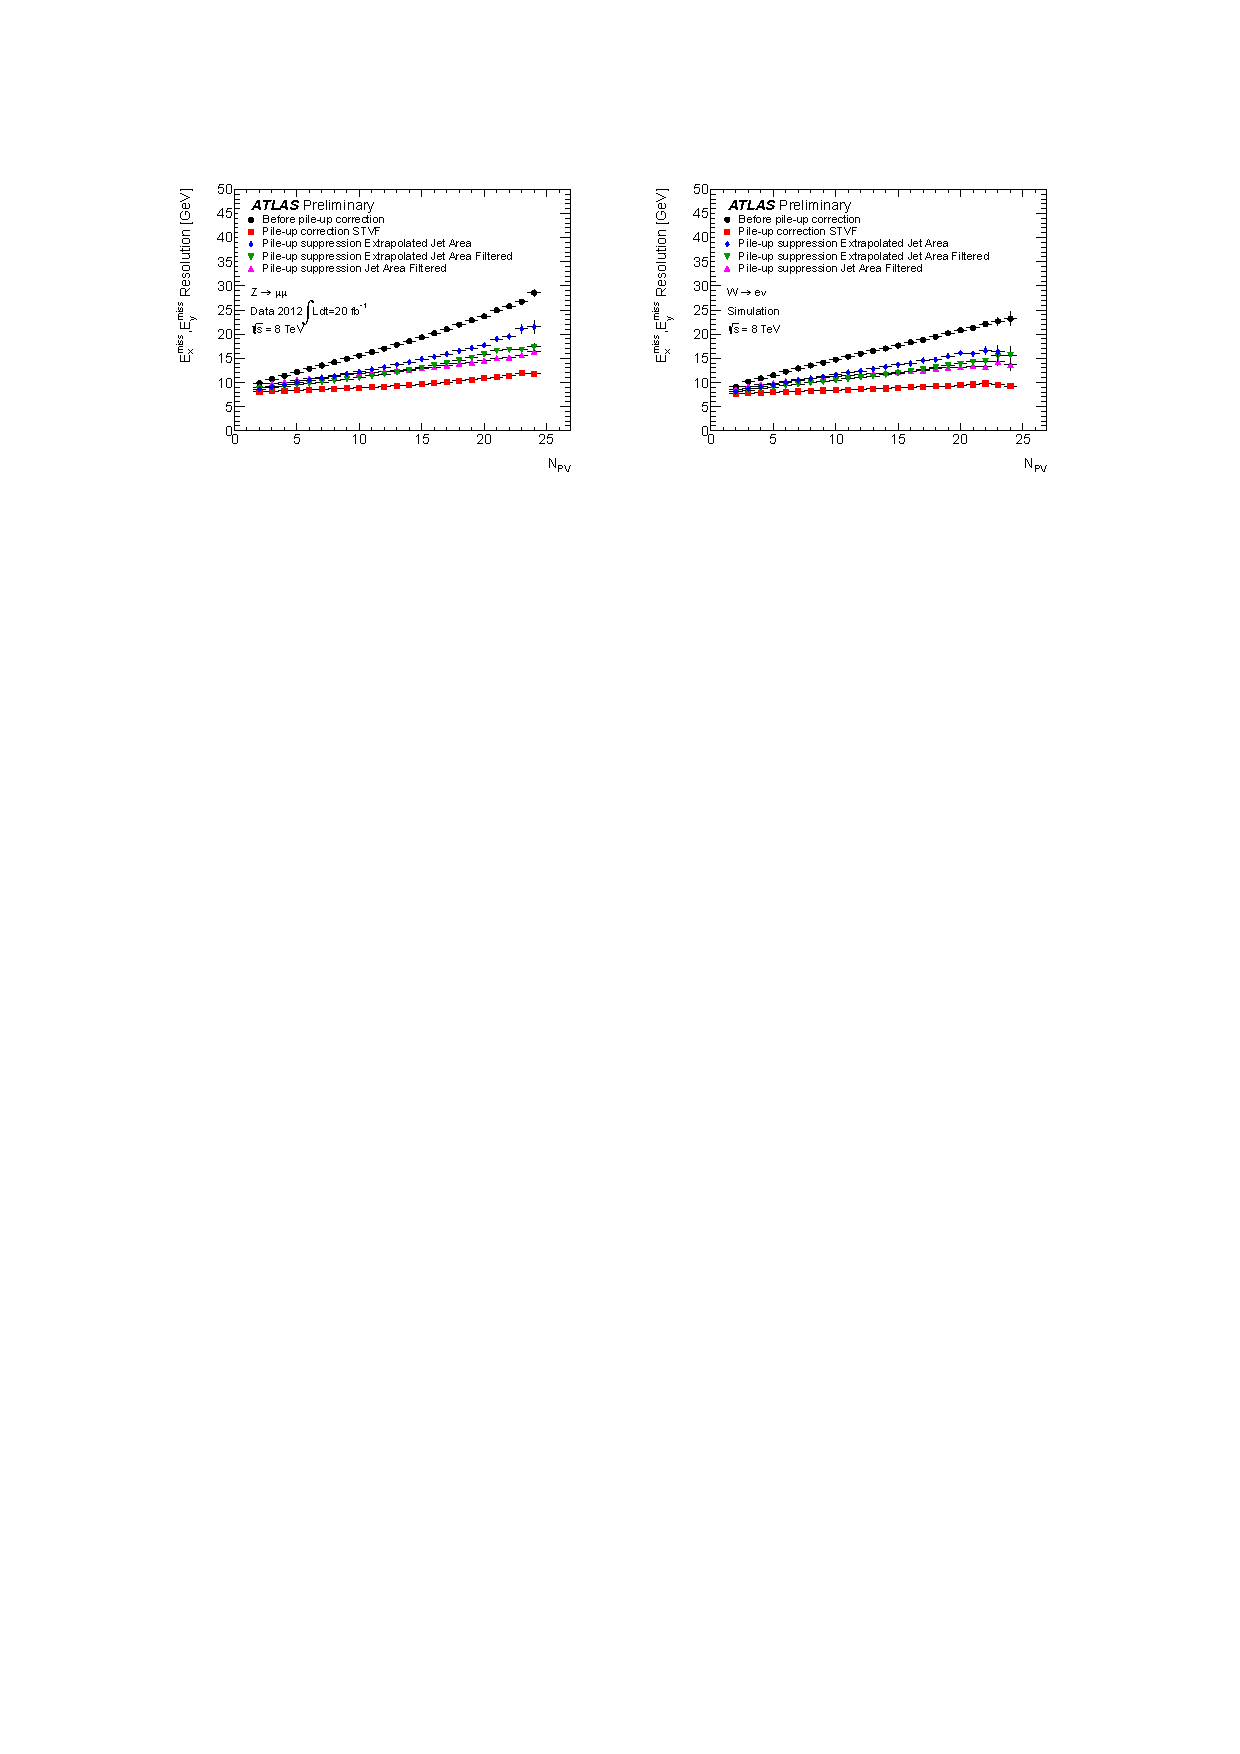
\includegraphics[width=0.90\textwidth]{figures/performance/met-resolutionvsnpv}
  \caption{Variables.}
  \label{fig:strategy-objects-met-resolution}
\end{figure}

\begin{figure}[tp]
  \centering
  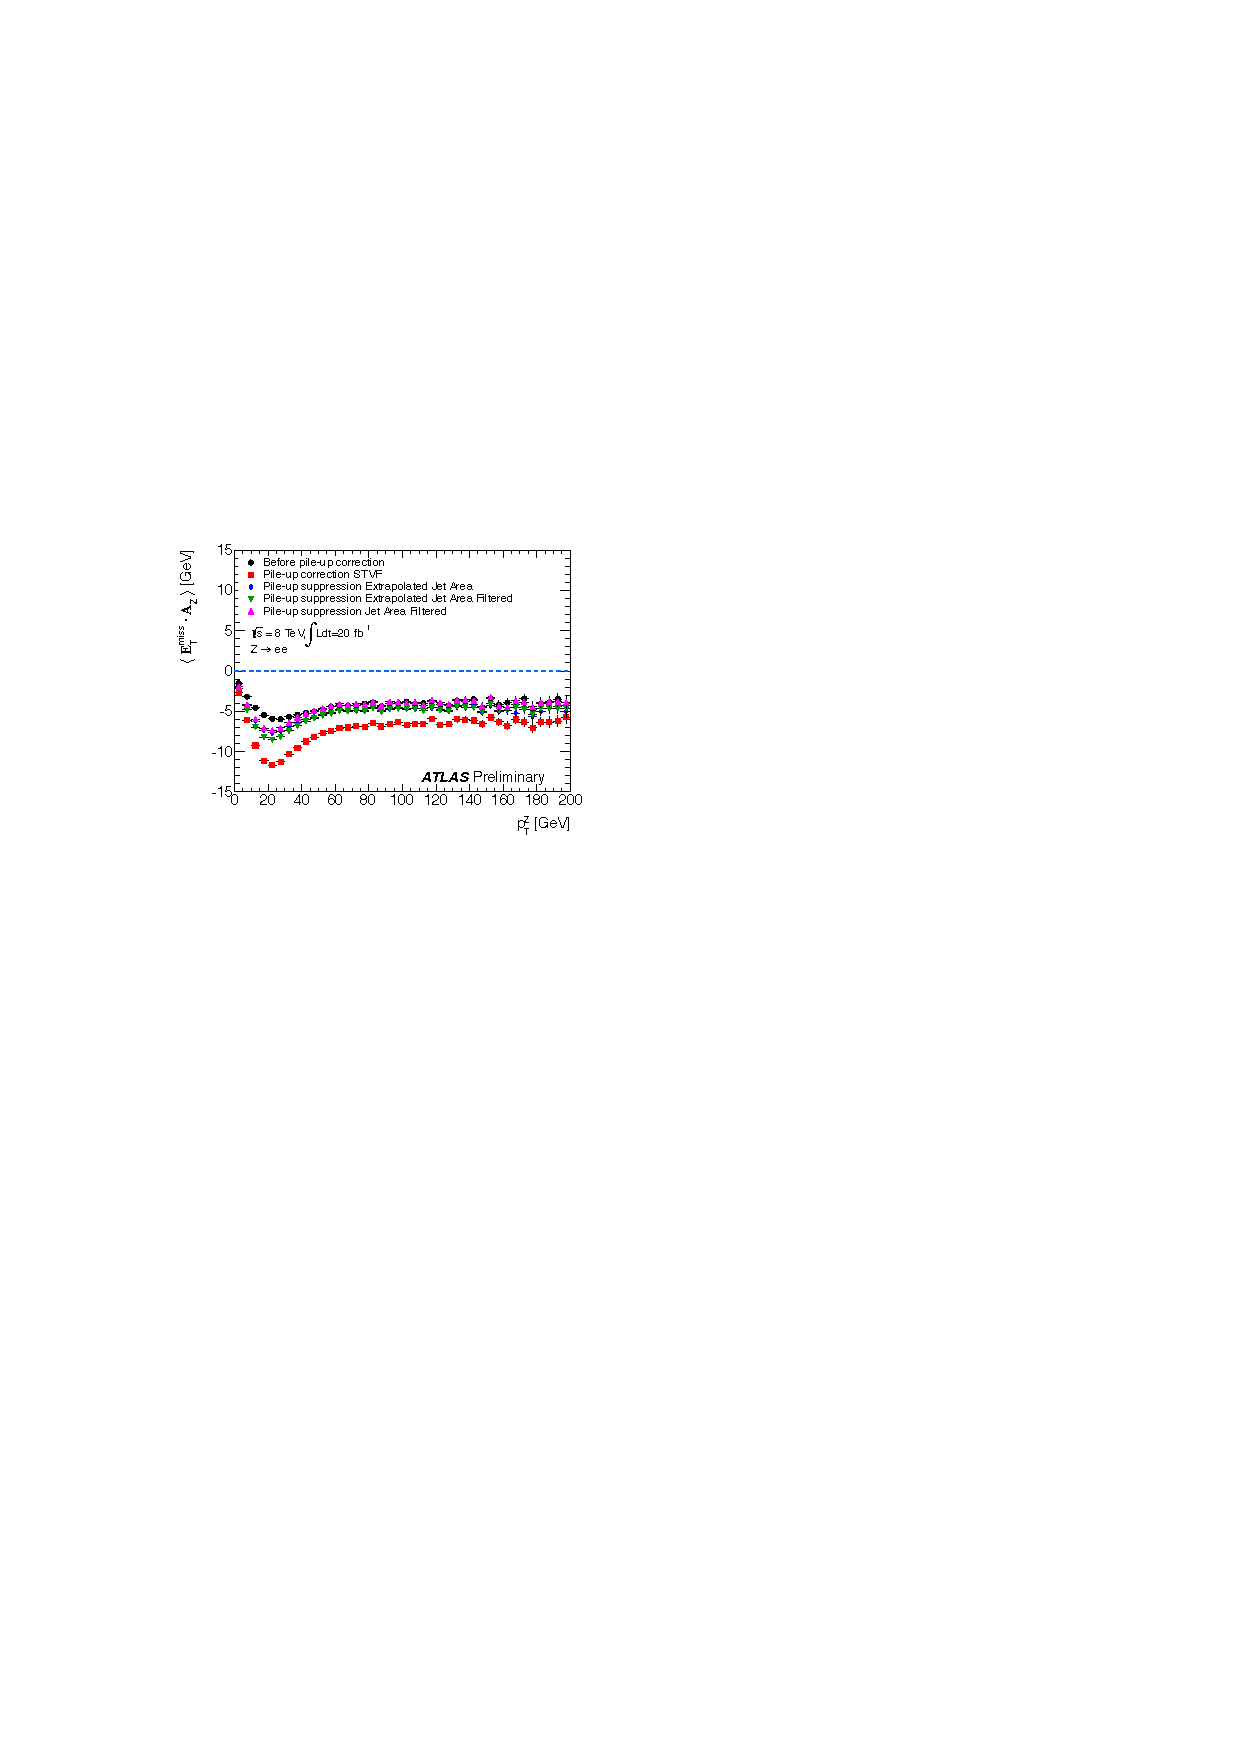
\includegraphics[width=0.48\textwidth]{figures/performance/met-bias-inclusive}
  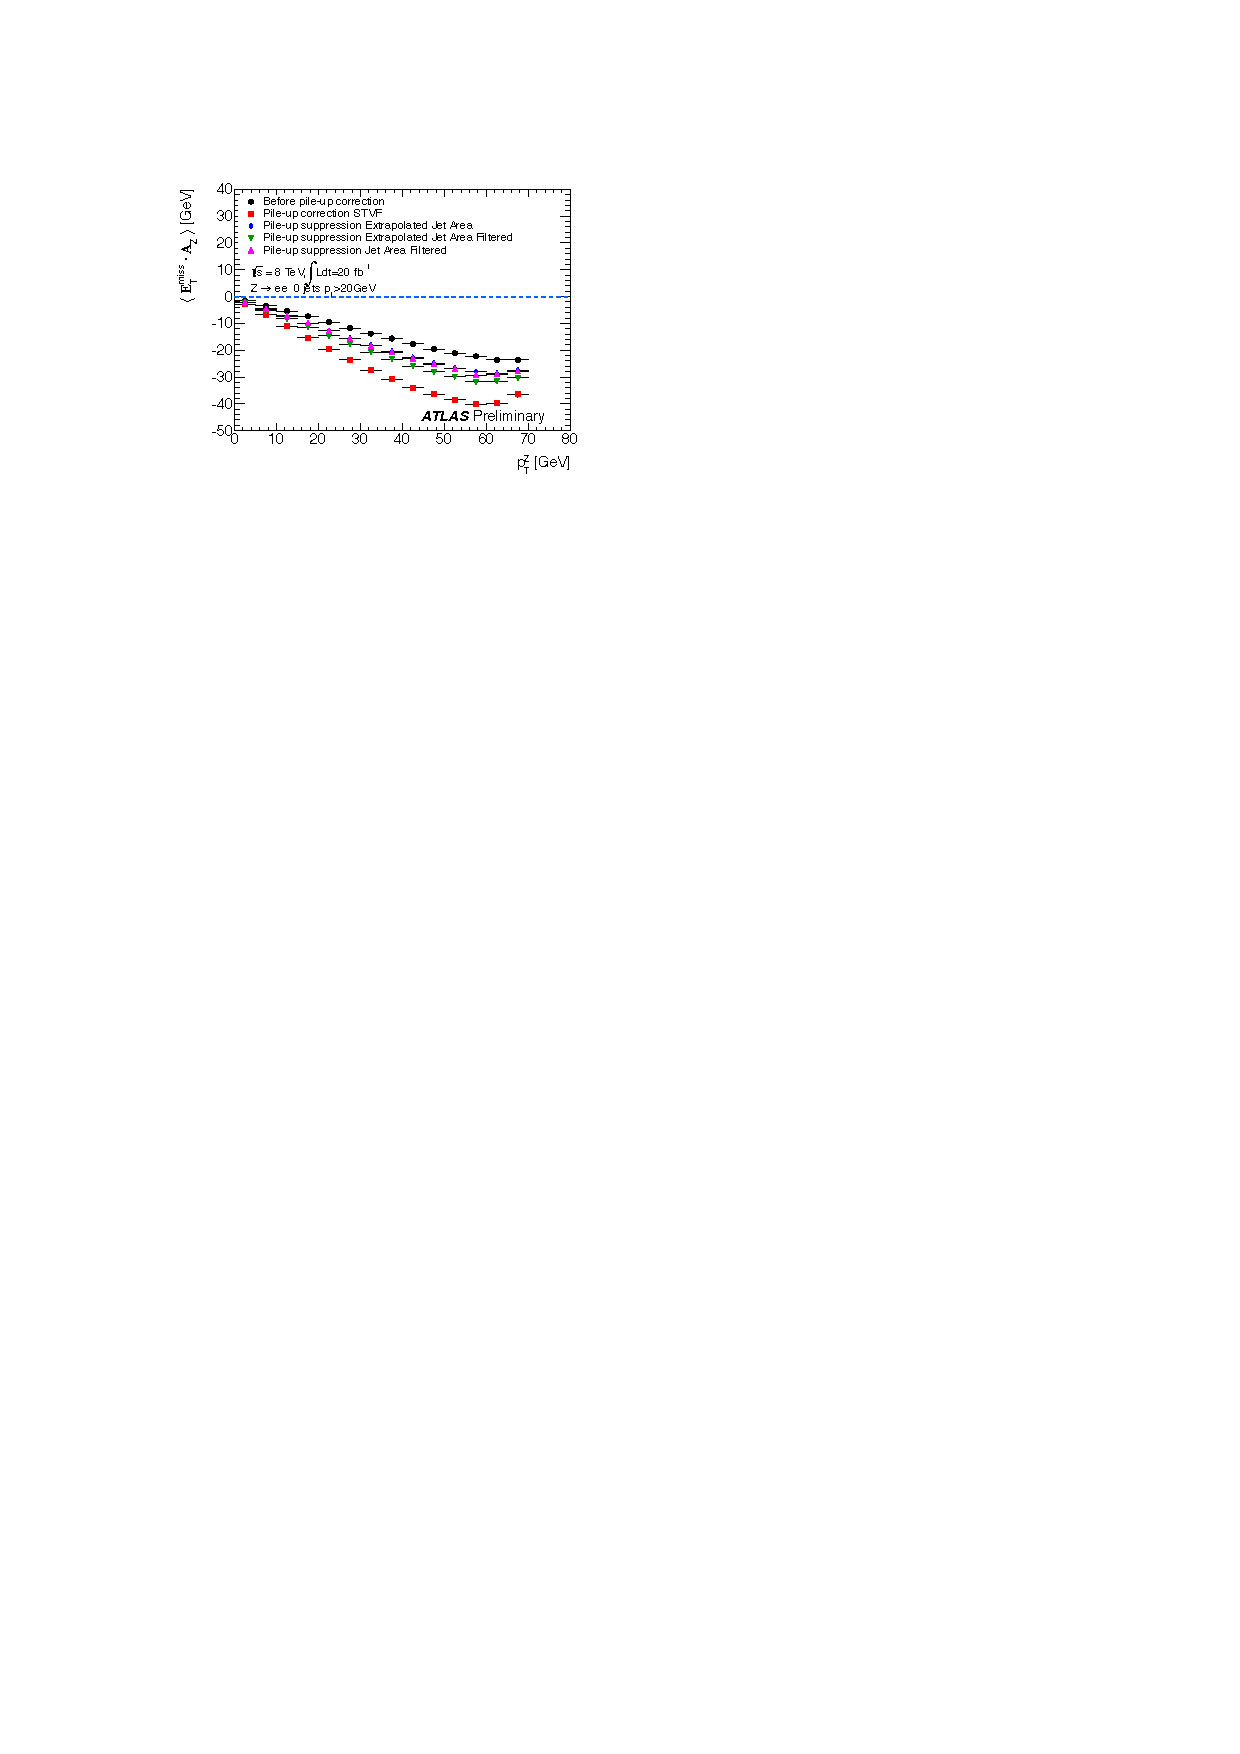
\includegraphics[width=0.48\textwidth]{figures/performance/met-bias-0jet}
  \caption{Variables.}
  \label{fig:strategy-objects-met-bias}
\end{figure}

\begin{figure}[tp]
  \centering
  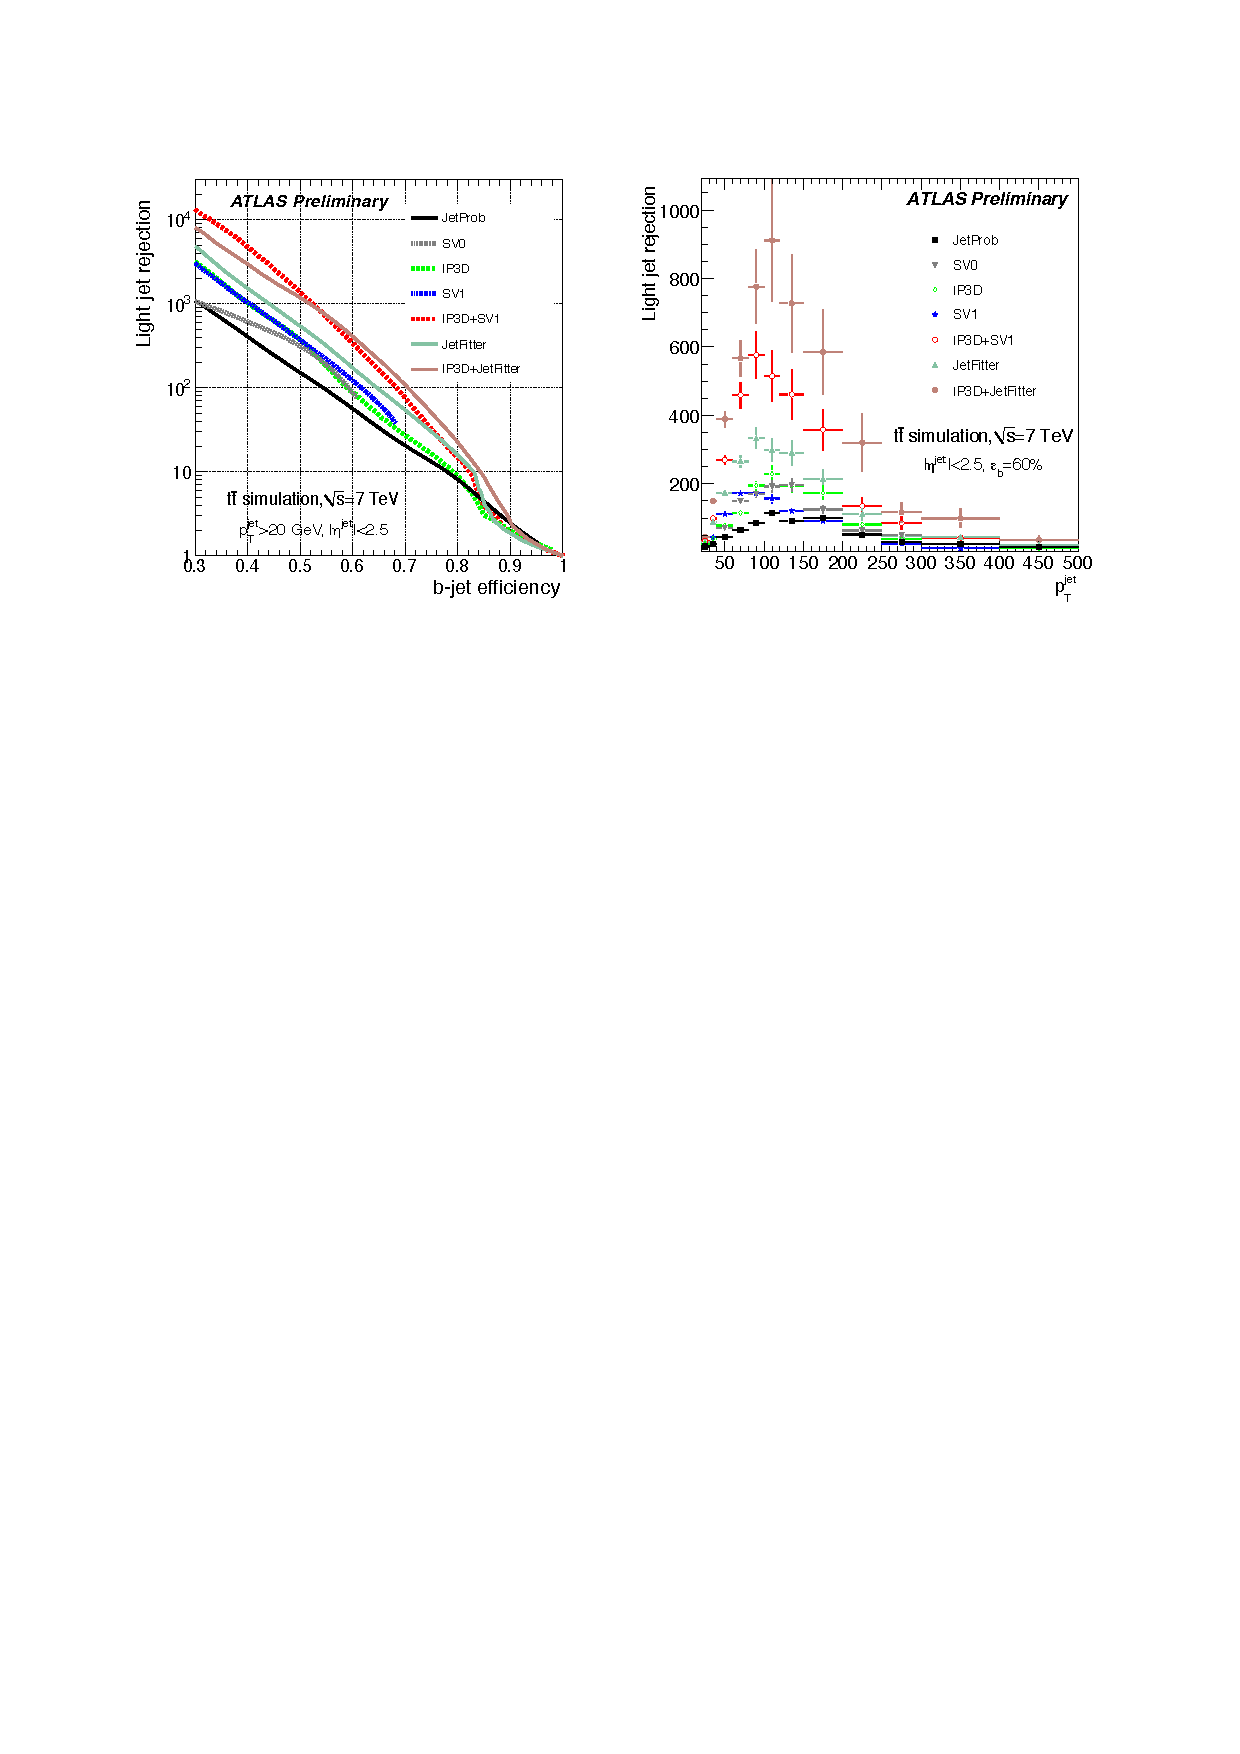
\includegraphics[width=0.90\textwidth]{figures/performance/btag-MCperformance}
  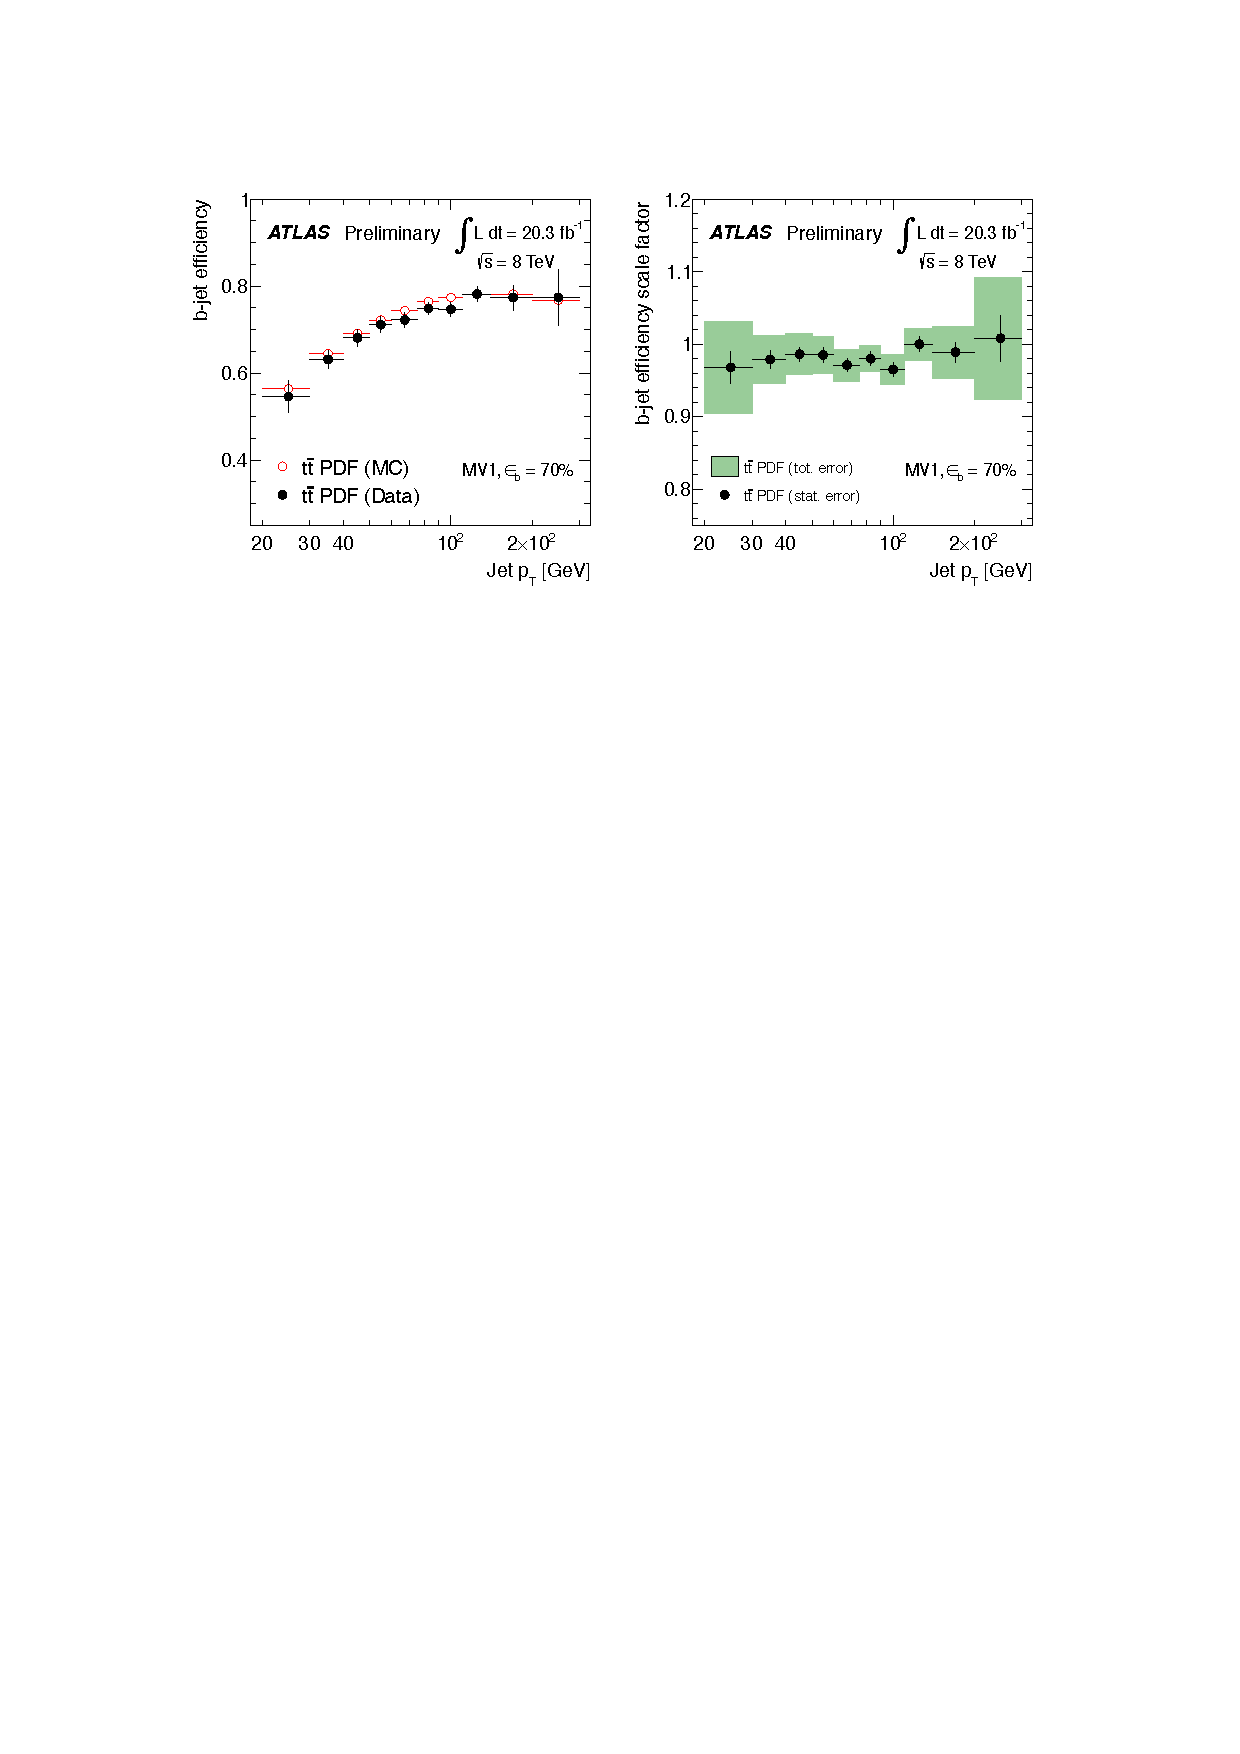
\includegraphics[width=0.90\textwidth]{figures/performance/btag-efficiency}
  \caption{Variables.}
  \label{fig:strategy-objects-btag}
\end{figure}

\section{Categorization}
\label{sec:strategy-categorization}

\begin{figure}[tp]
  \centering
  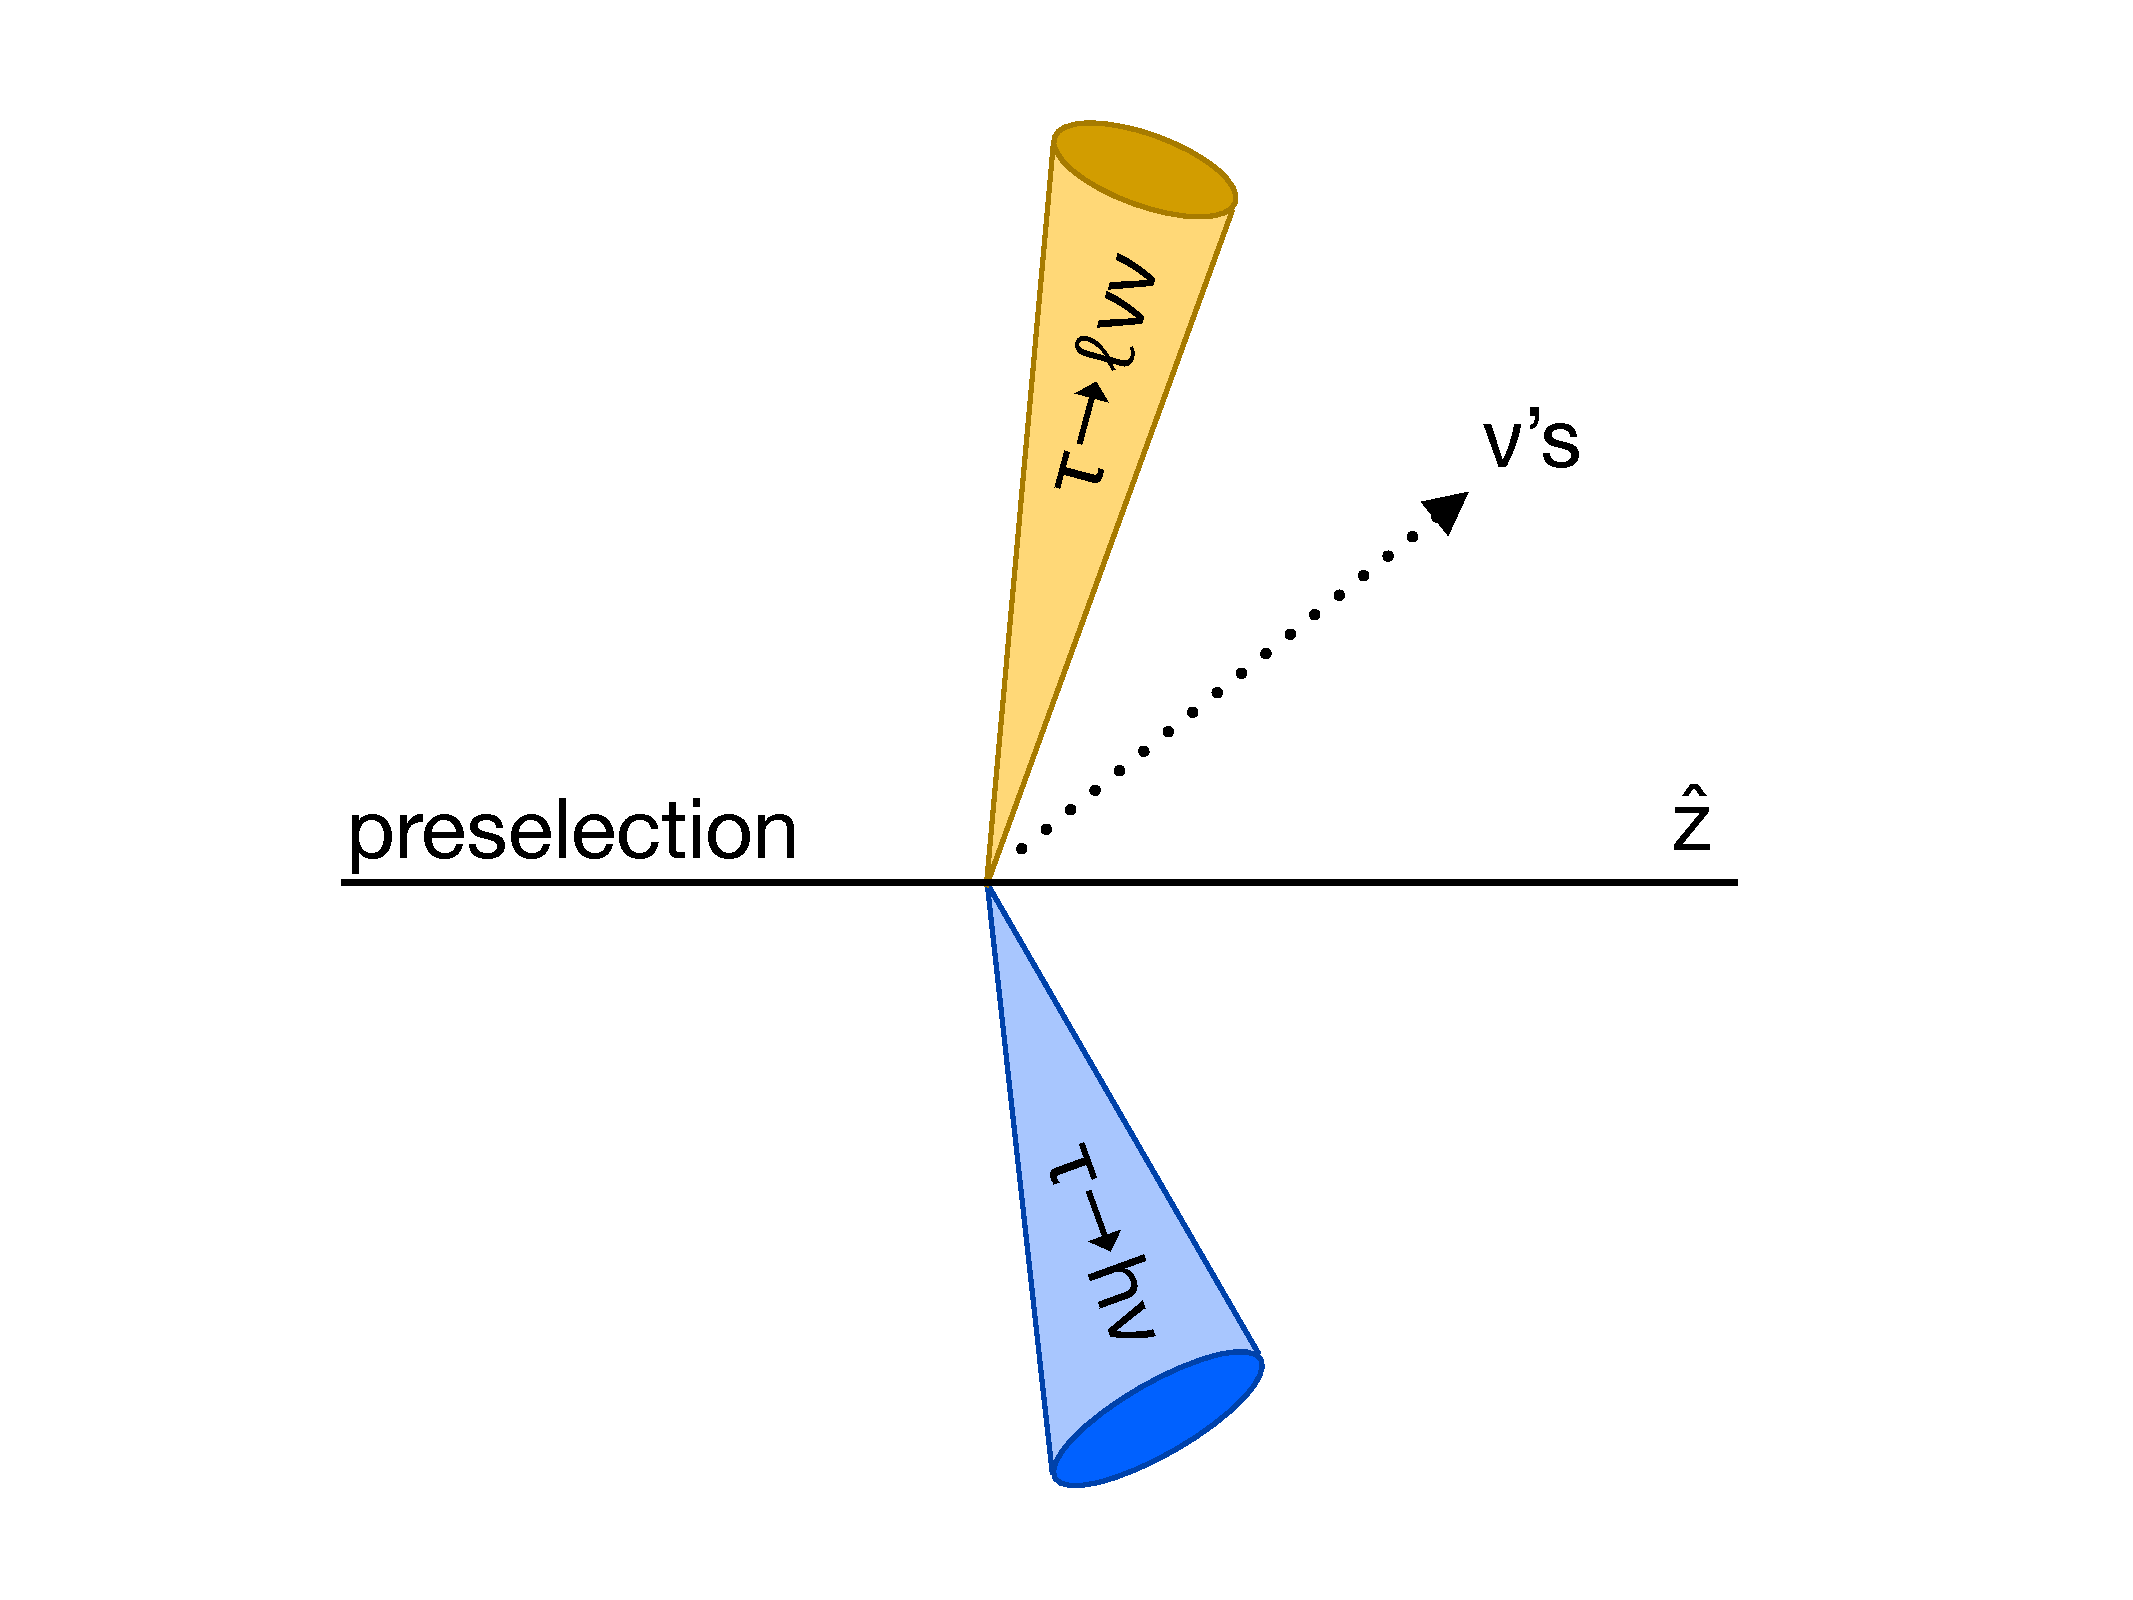
\includegraphics[width=0.48\textwidth]{figures/category-cartoons/presel}
  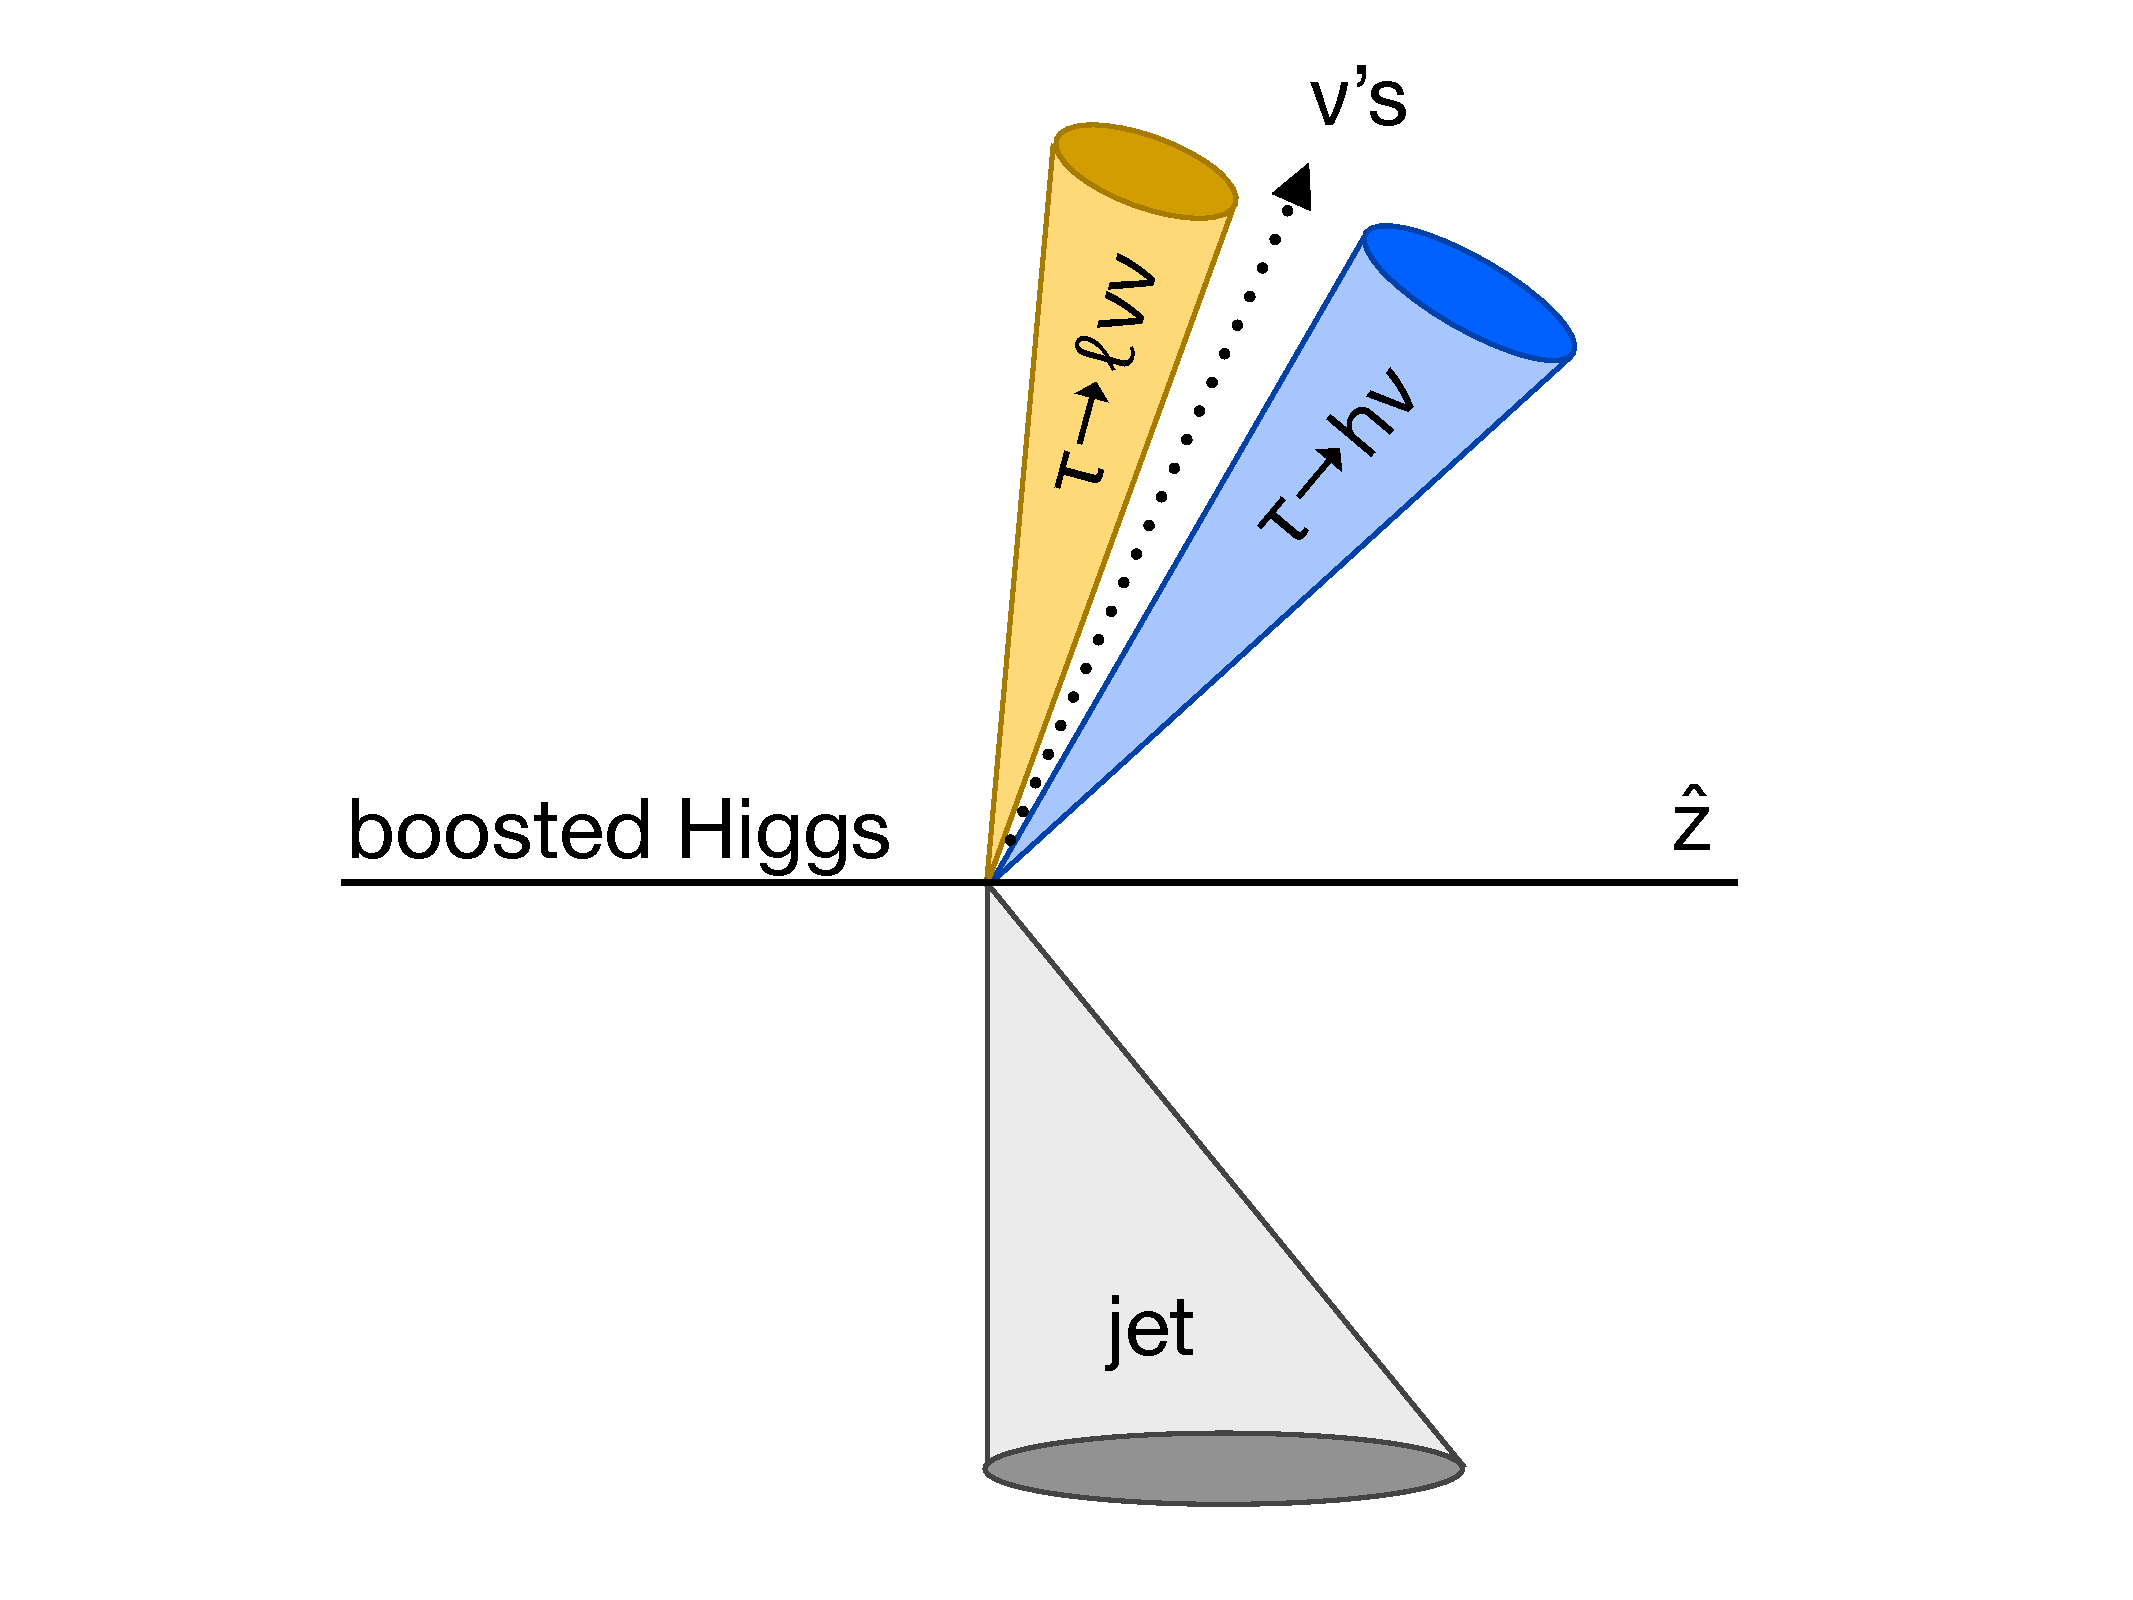
\includegraphics[width=0.48\textwidth]{figures/category-cartoons/boost}
  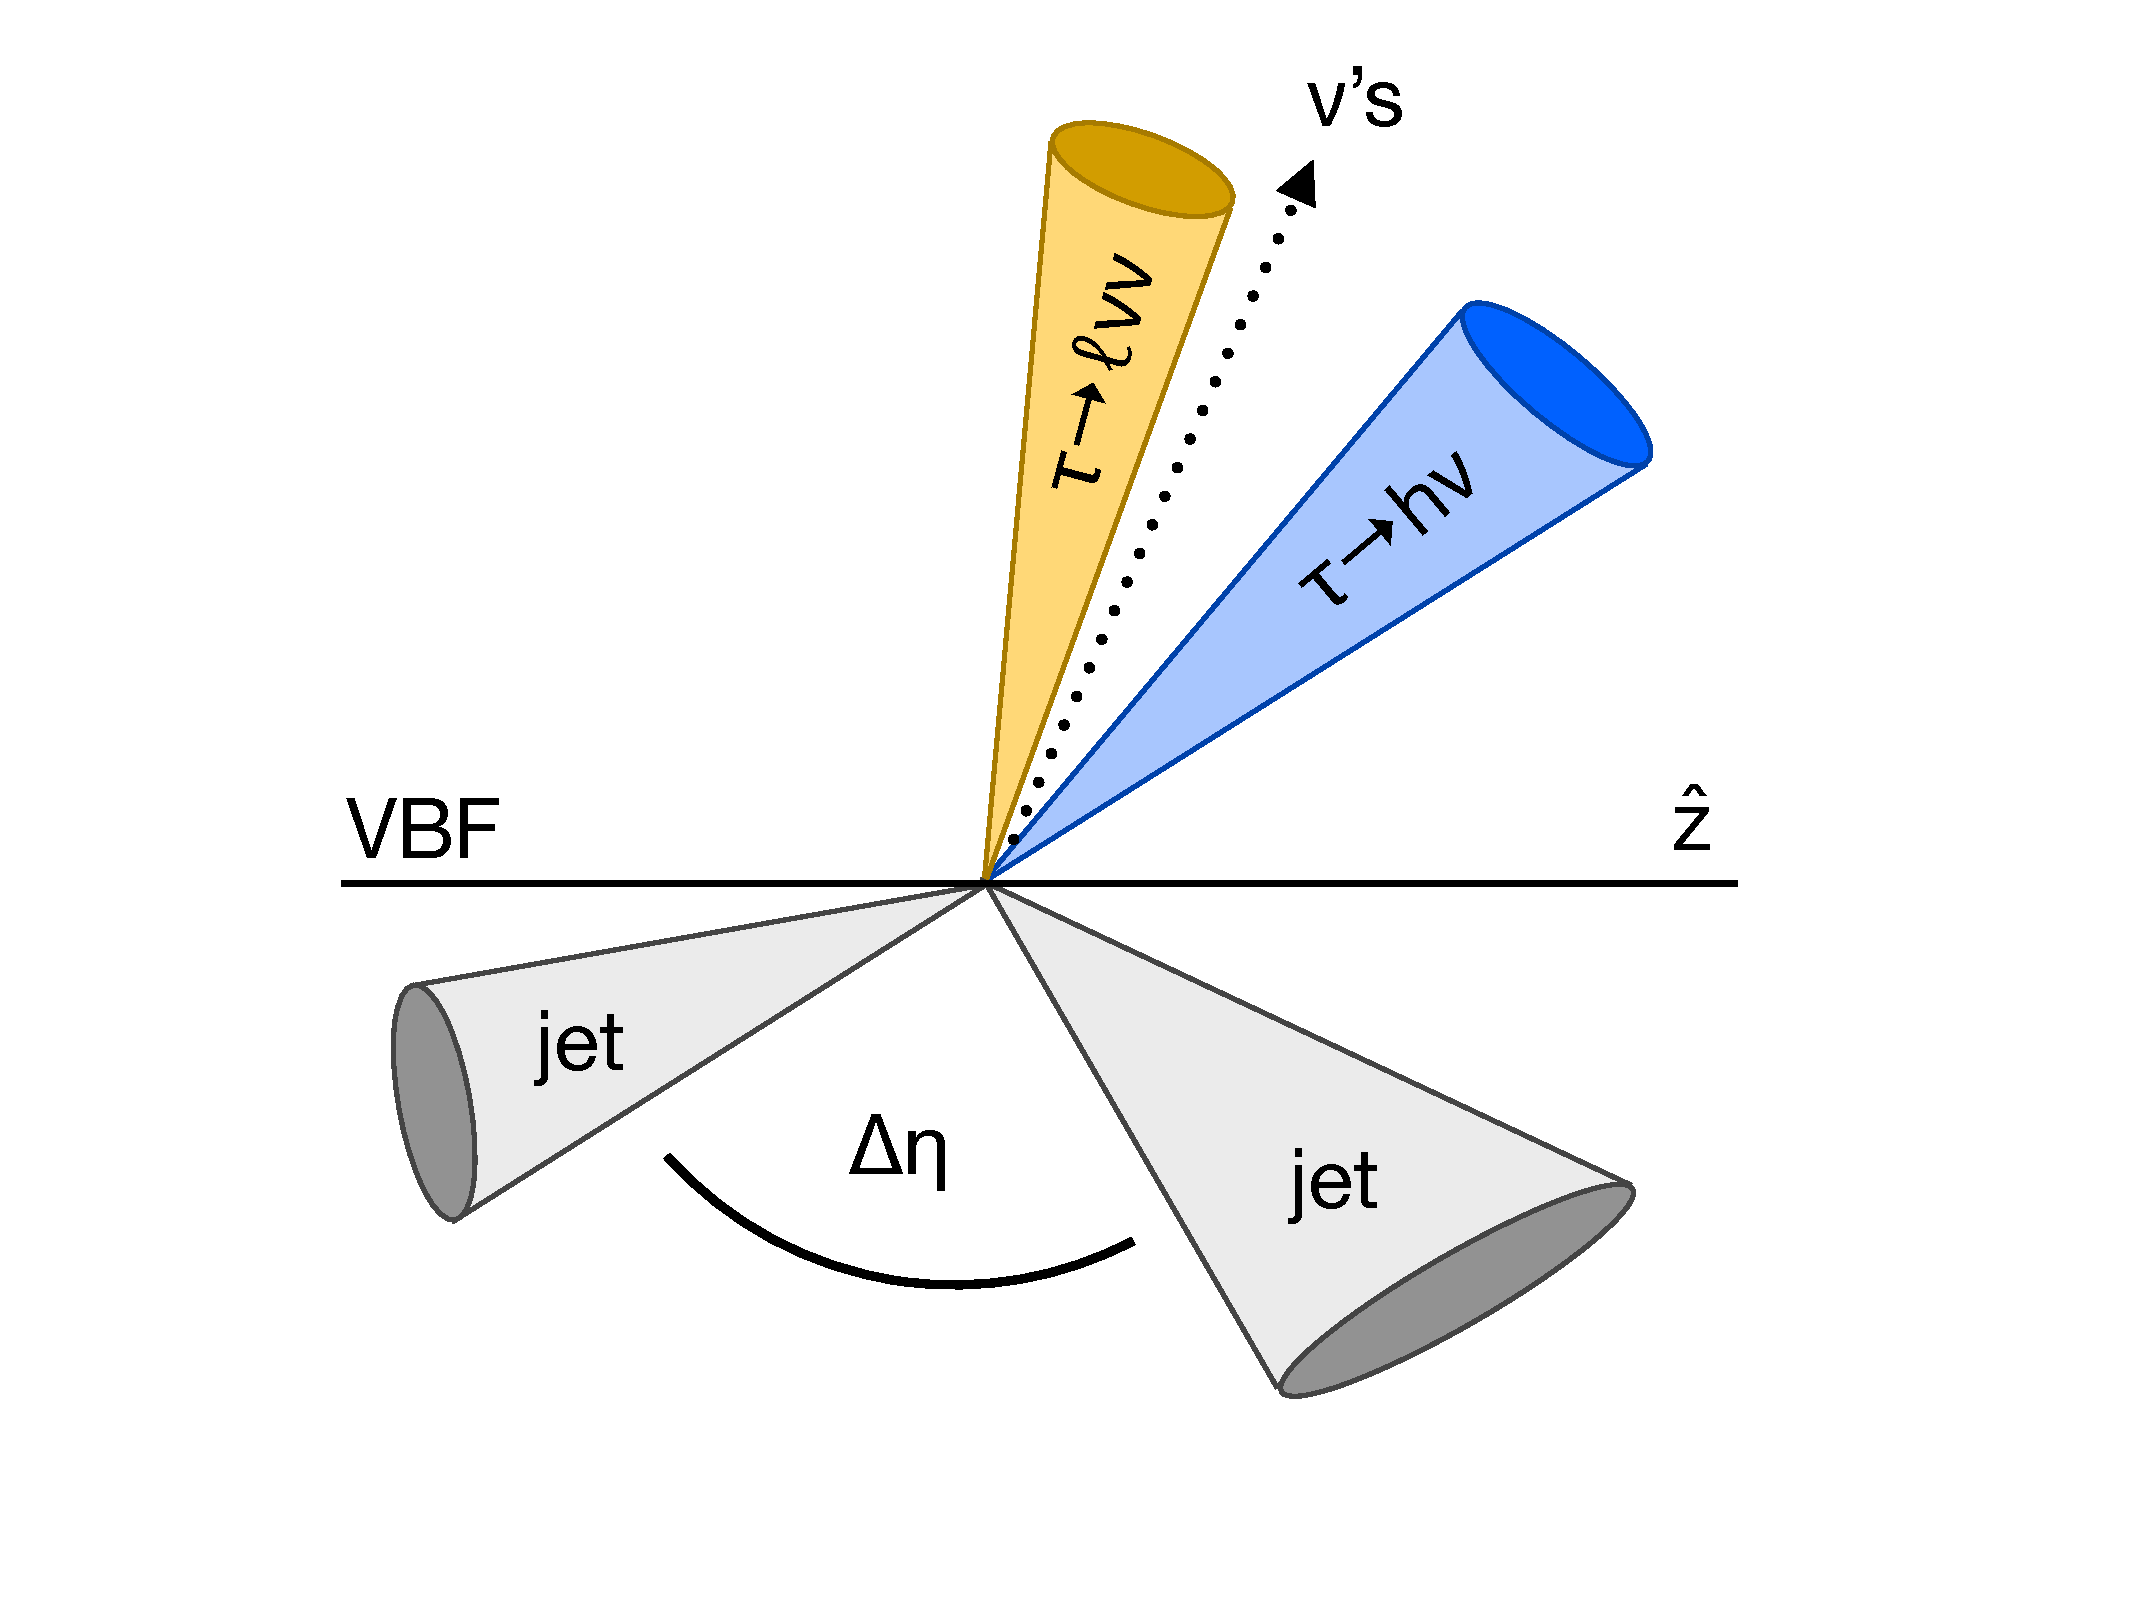
\includegraphics[width=0.48\textwidth]{figures/category-cartoons/vbf}
  \caption{Variables.}
  \label{fig:strategy-category-cartoons}
\end{figure}

\clearpage
\begin{figure}[tp]
  \centering
  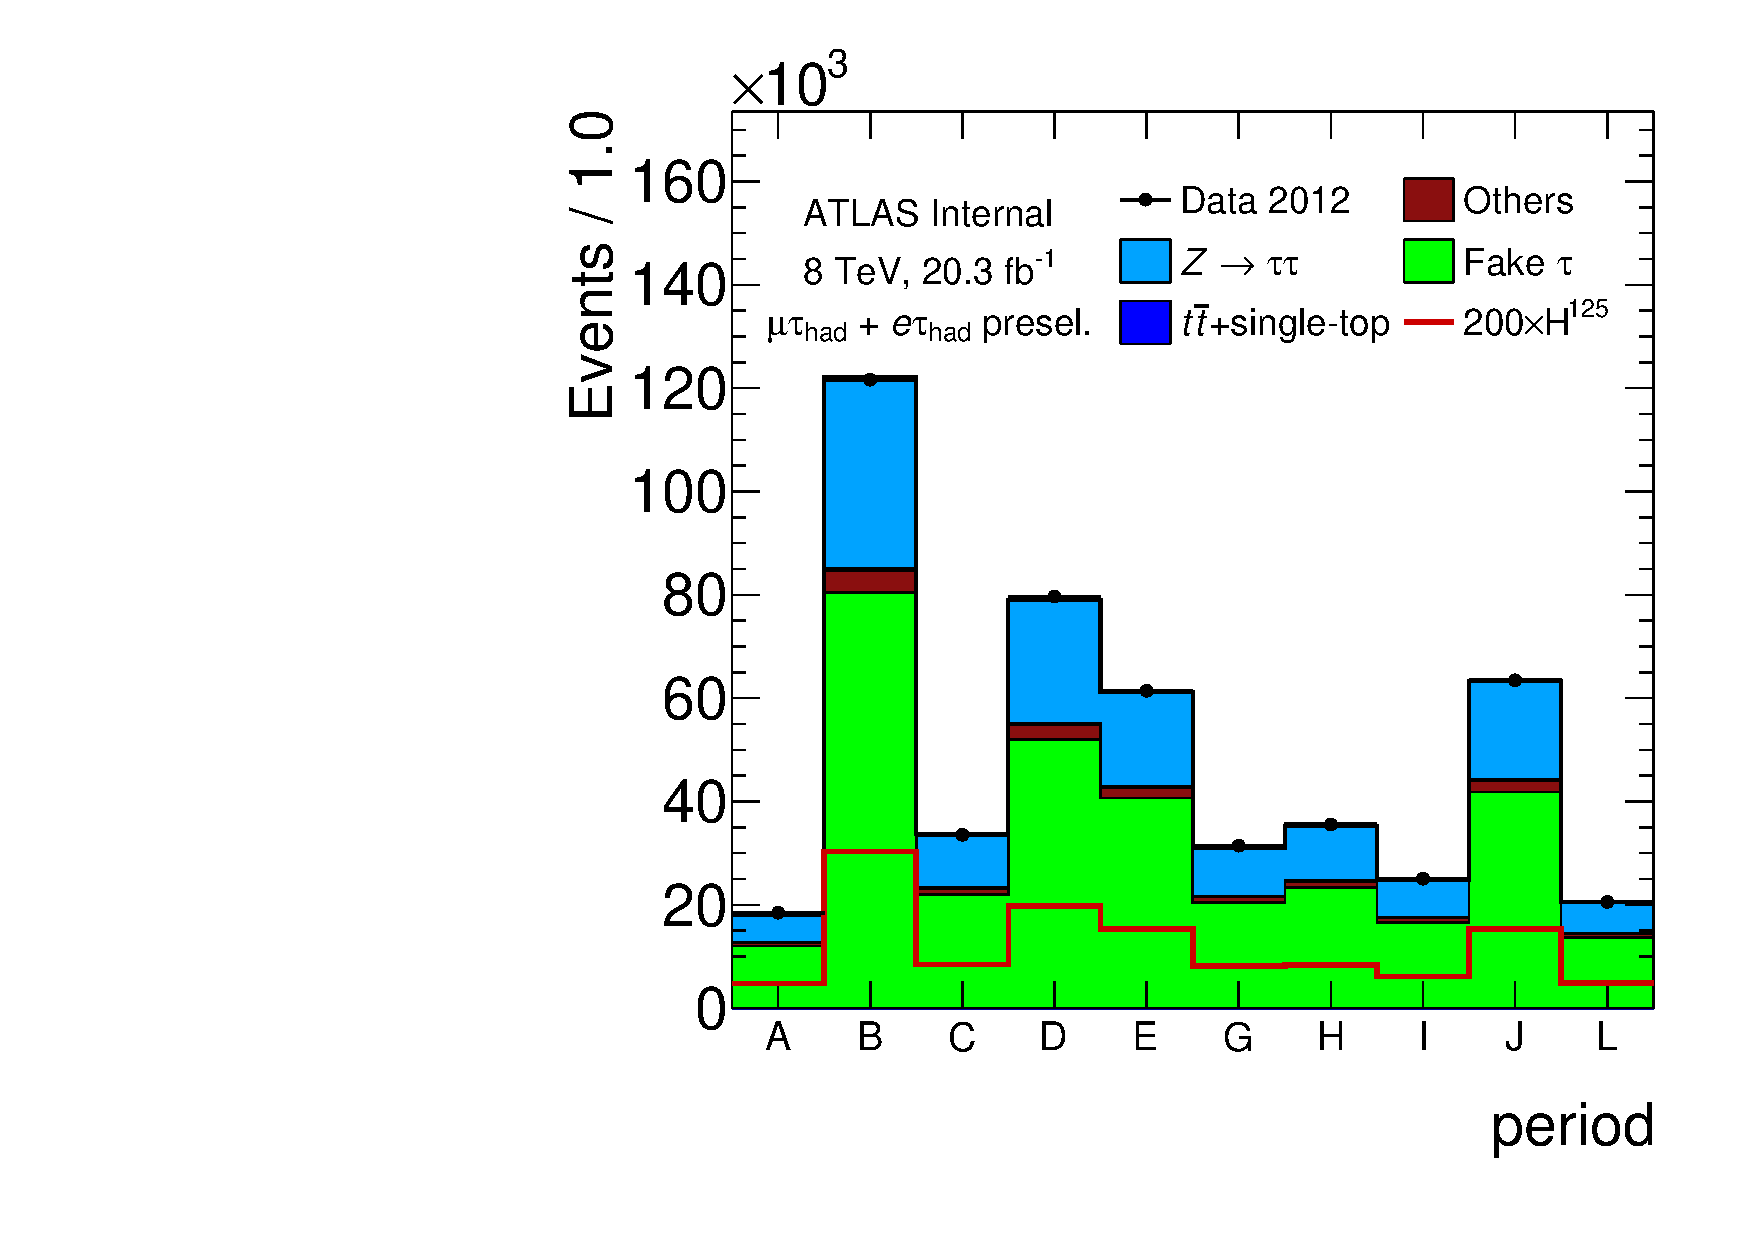
\includegraphics[width=0.32\textwidth]{figures/presel/period}
  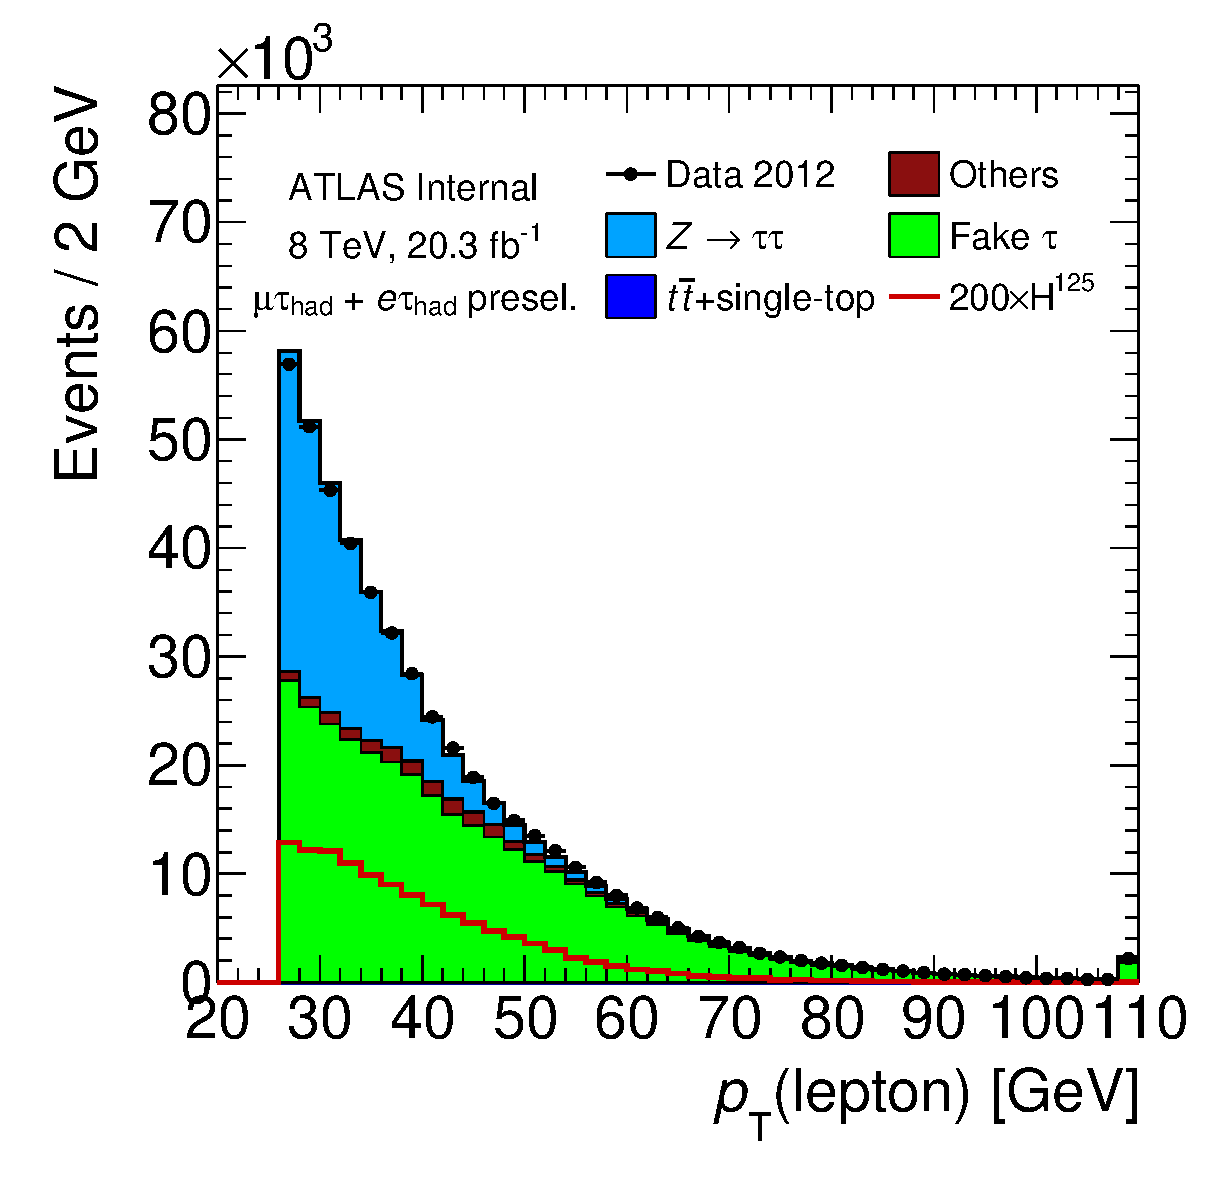
\includegraphics[width=0.32\textwidth]{figures/presel/lep-pt-hi}
  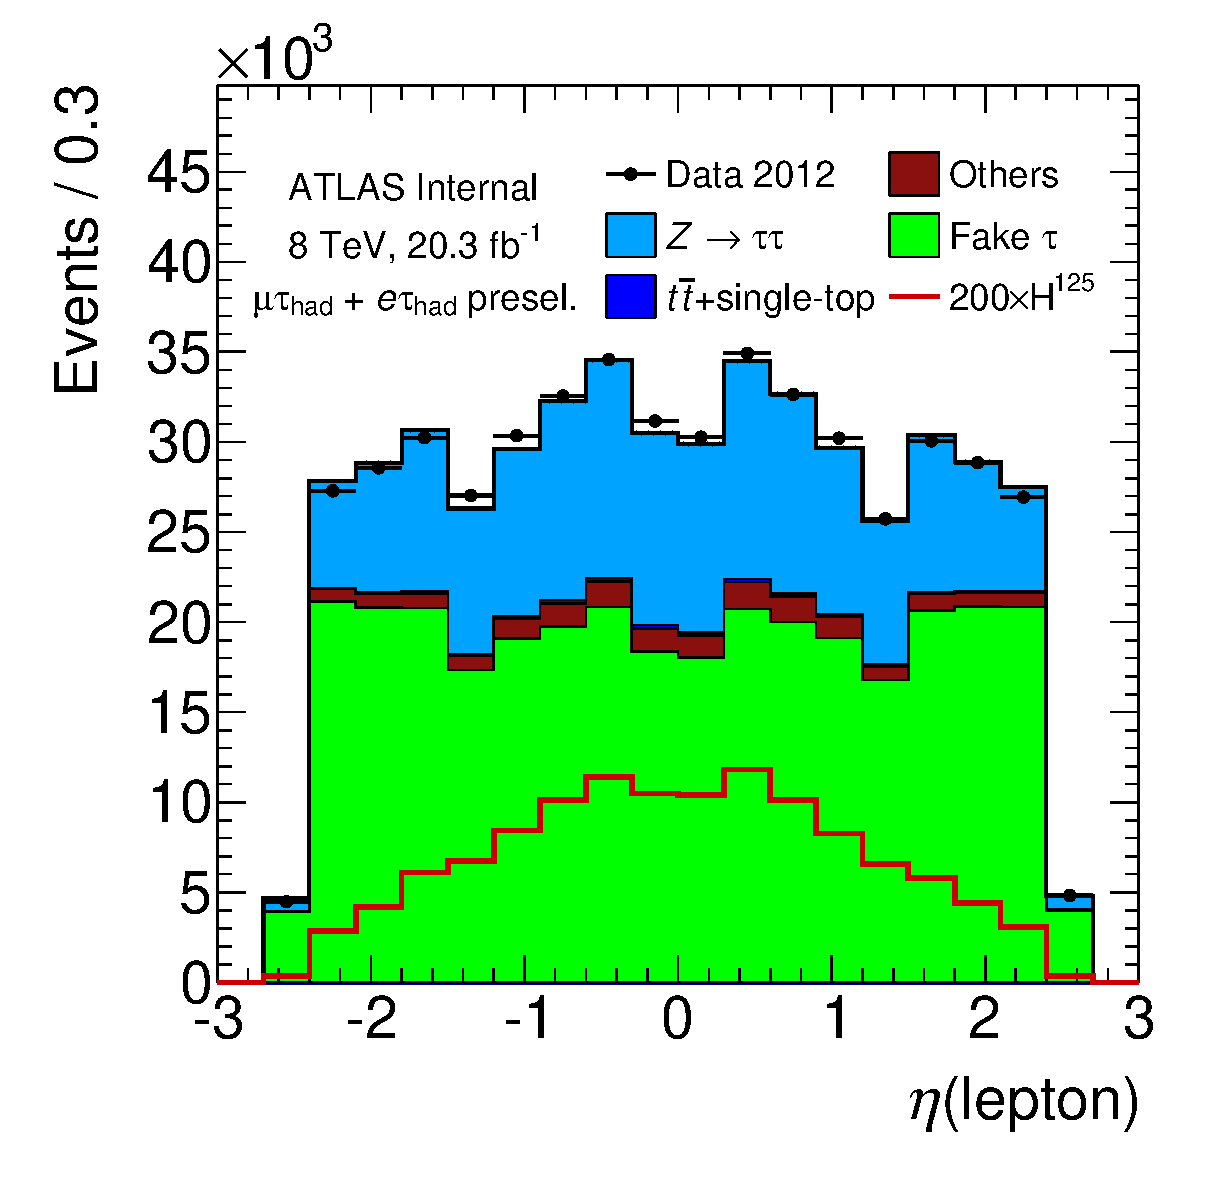
\includegraphics[width=0.32\textwidth]{figures/presel/lep-eta}
  % --------------
  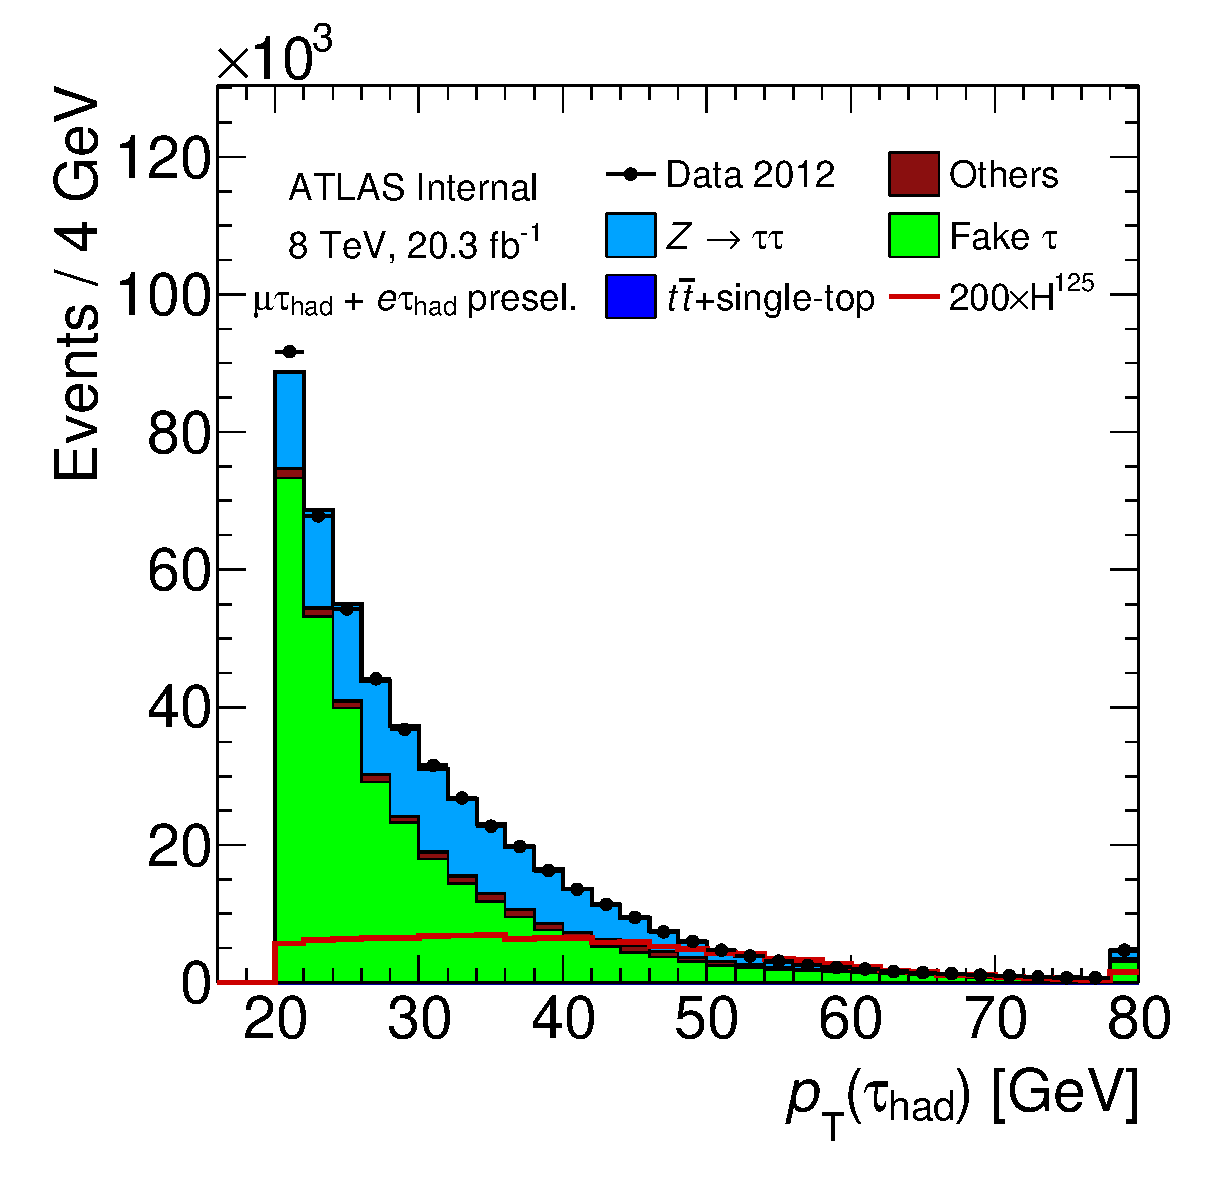
\includegraphics[width=0.32\textwidth]{figures/presel/tau-pt}
  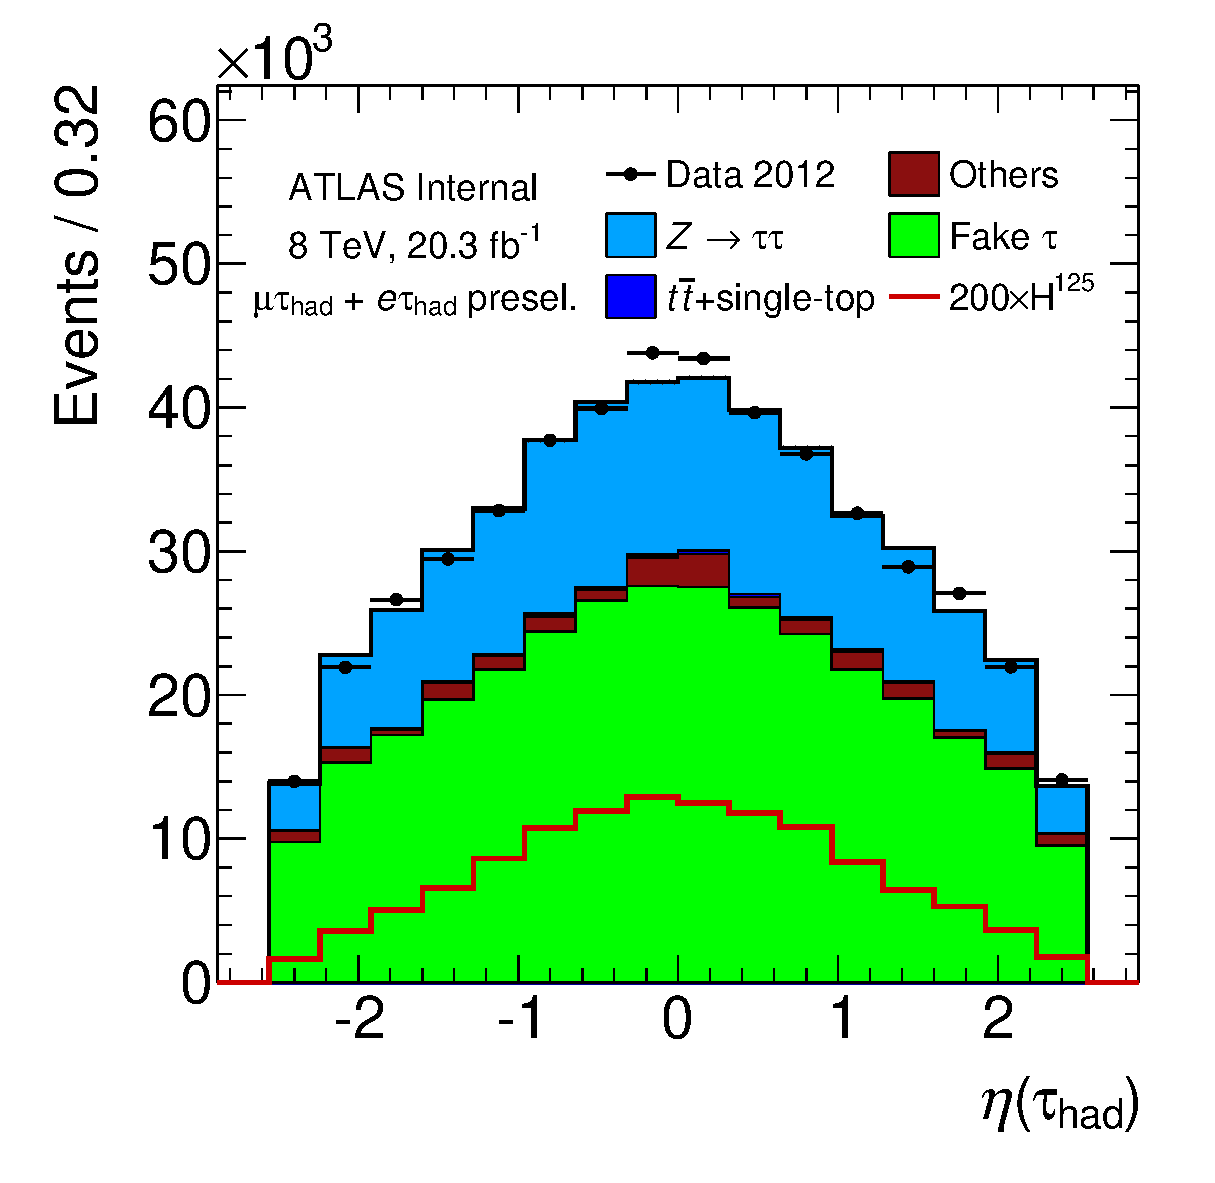
\includegraphics[width=0.32\textwidth]{figures/presel/tau-eta}
  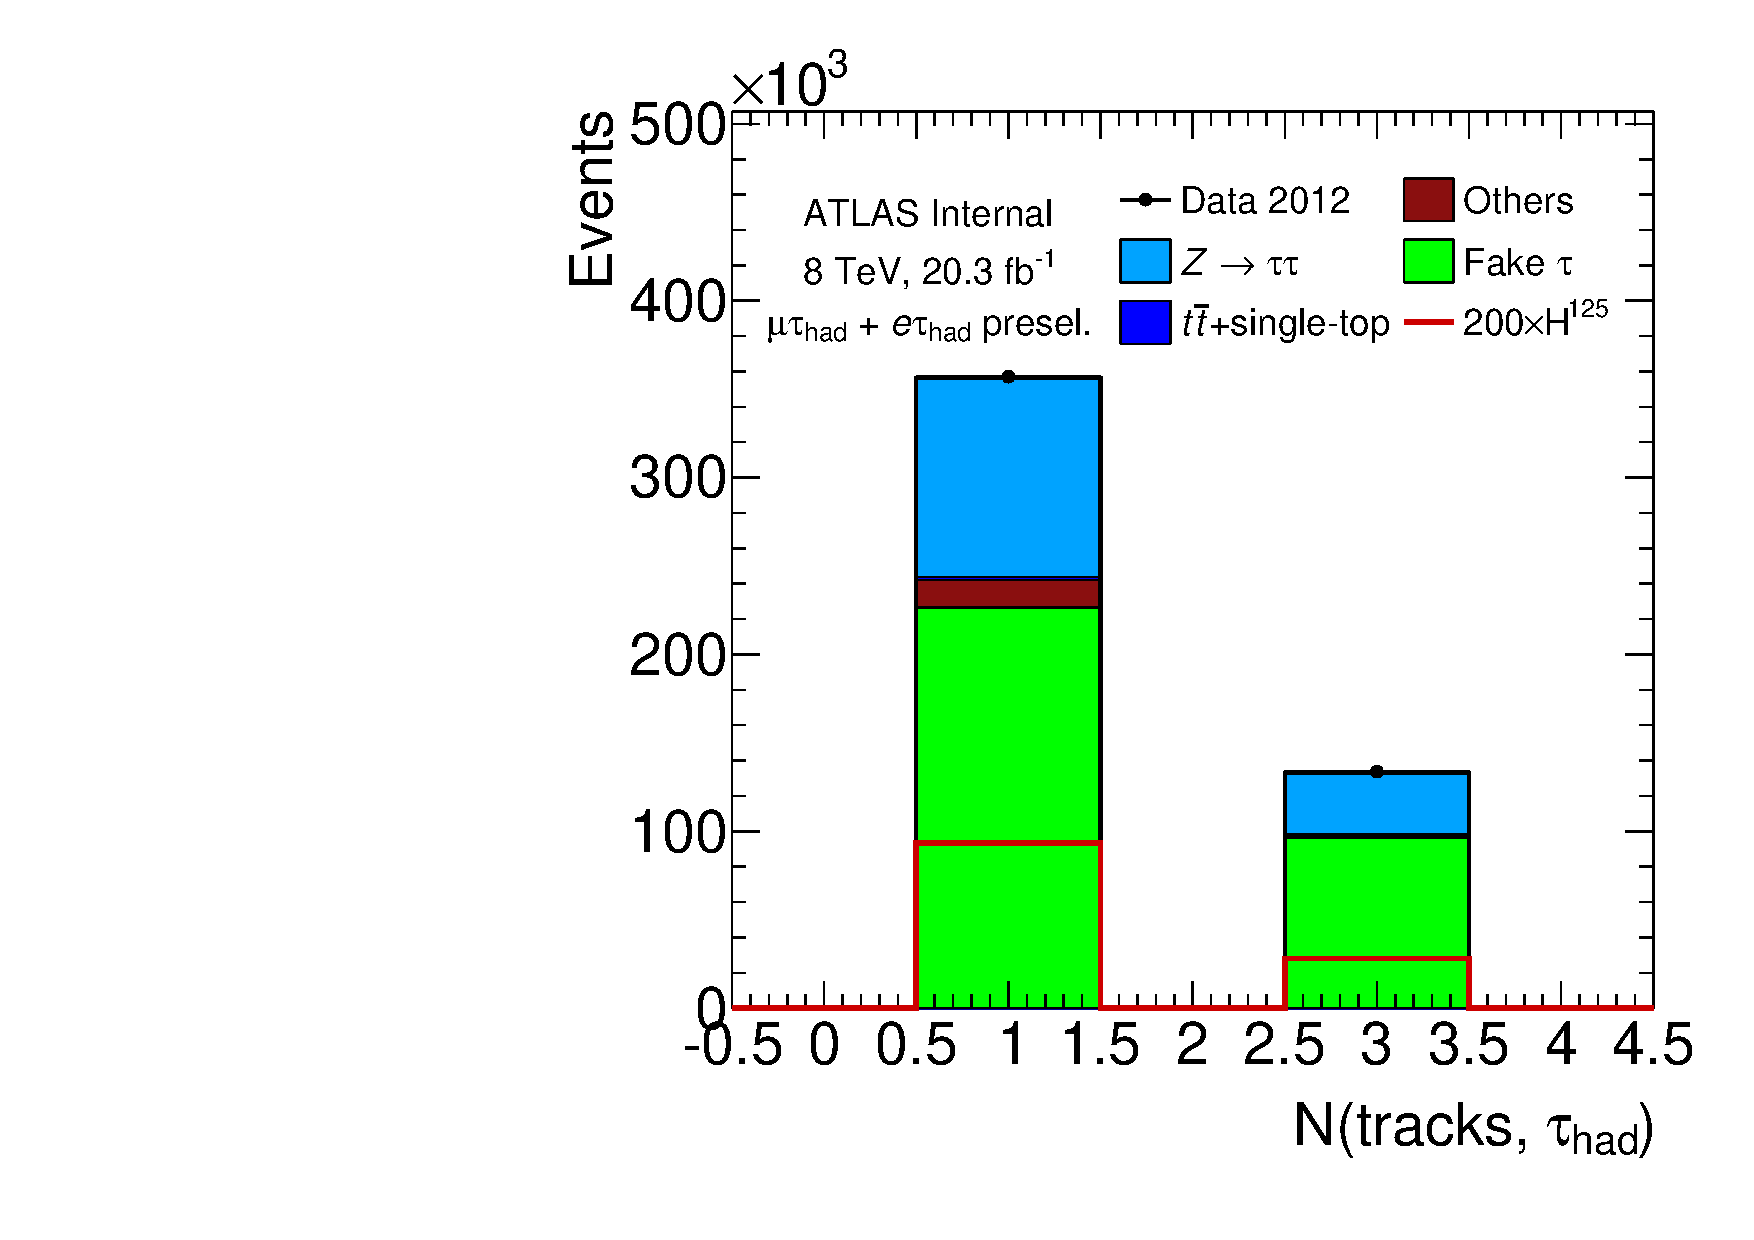
\includegraphics[width=0.32\textwidth]{figures/presel/tau-numTrack}
  % --------------
  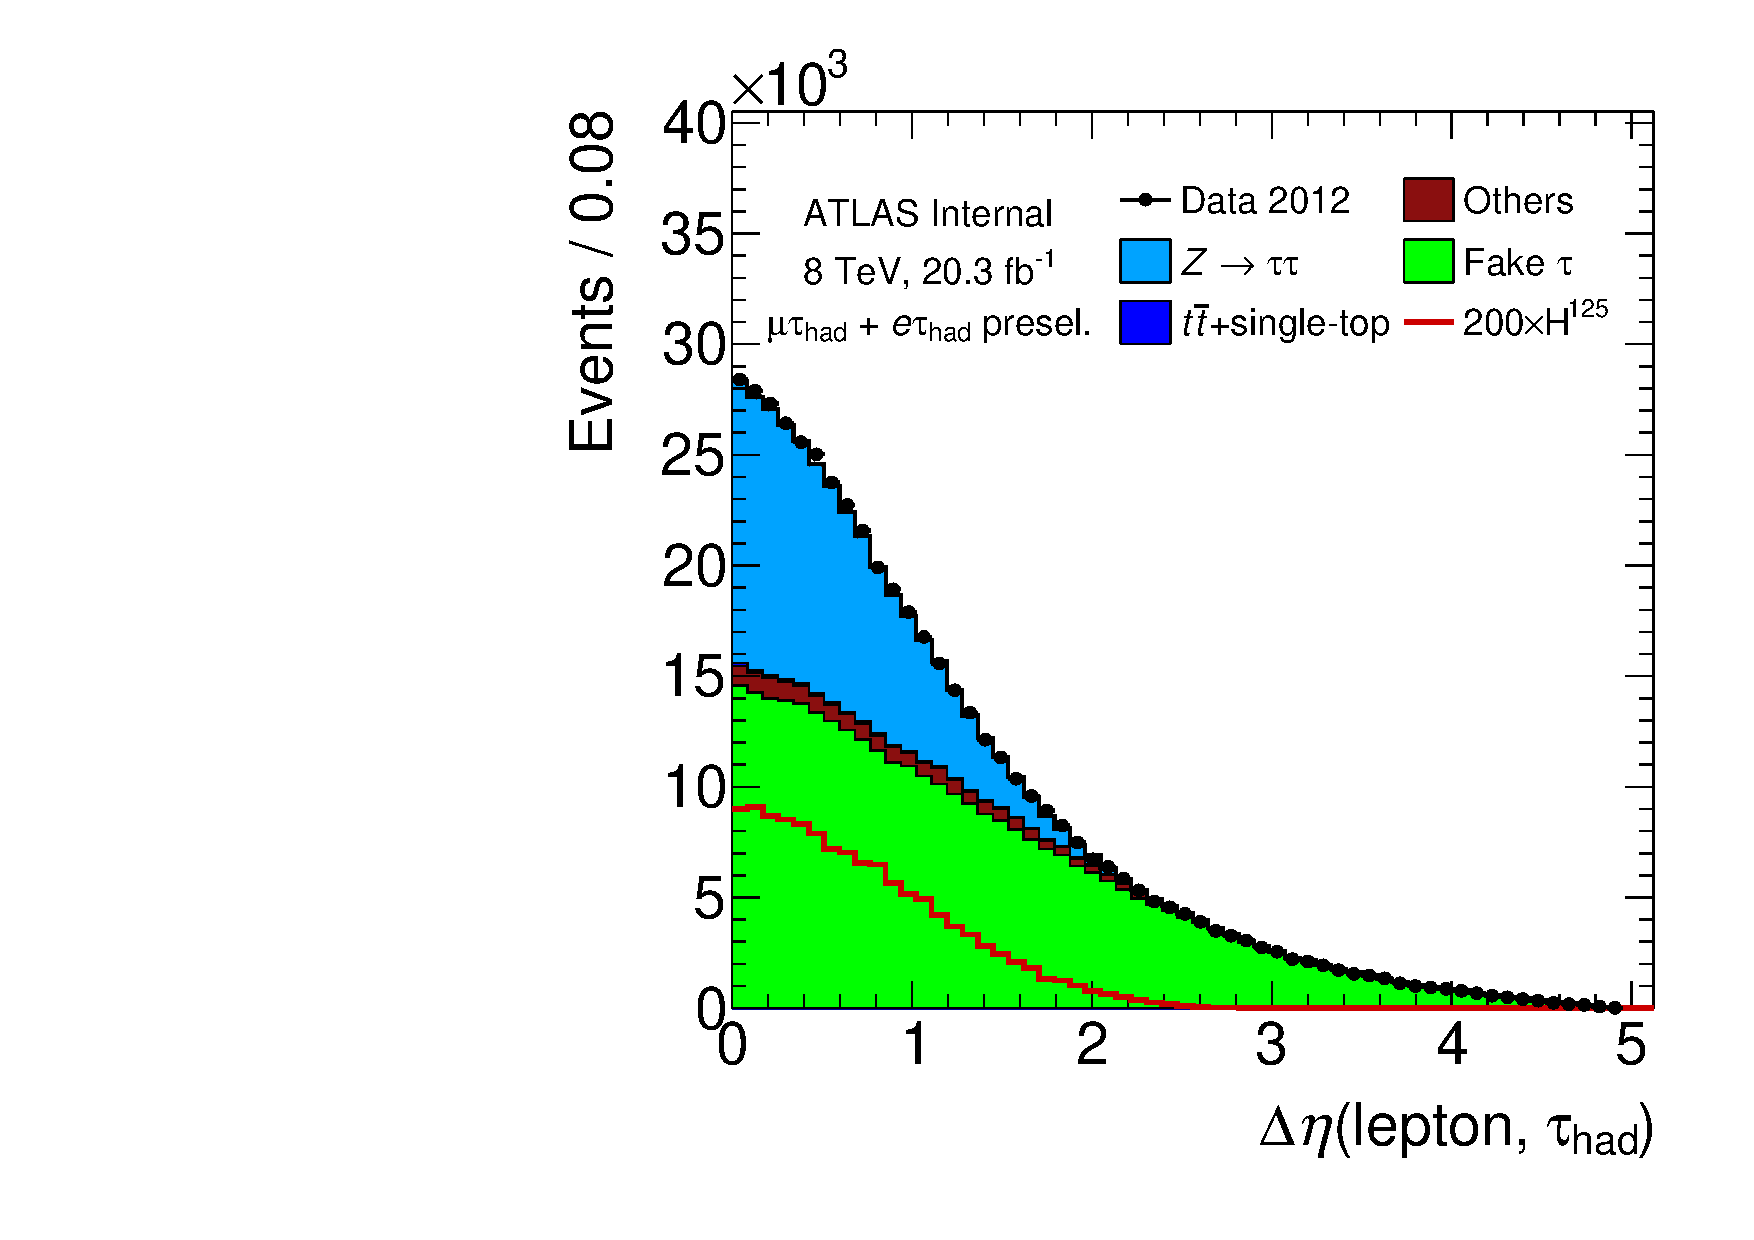
\includegraphics[width=0.32\textwidth]{figures/presel/taulep-deta}
  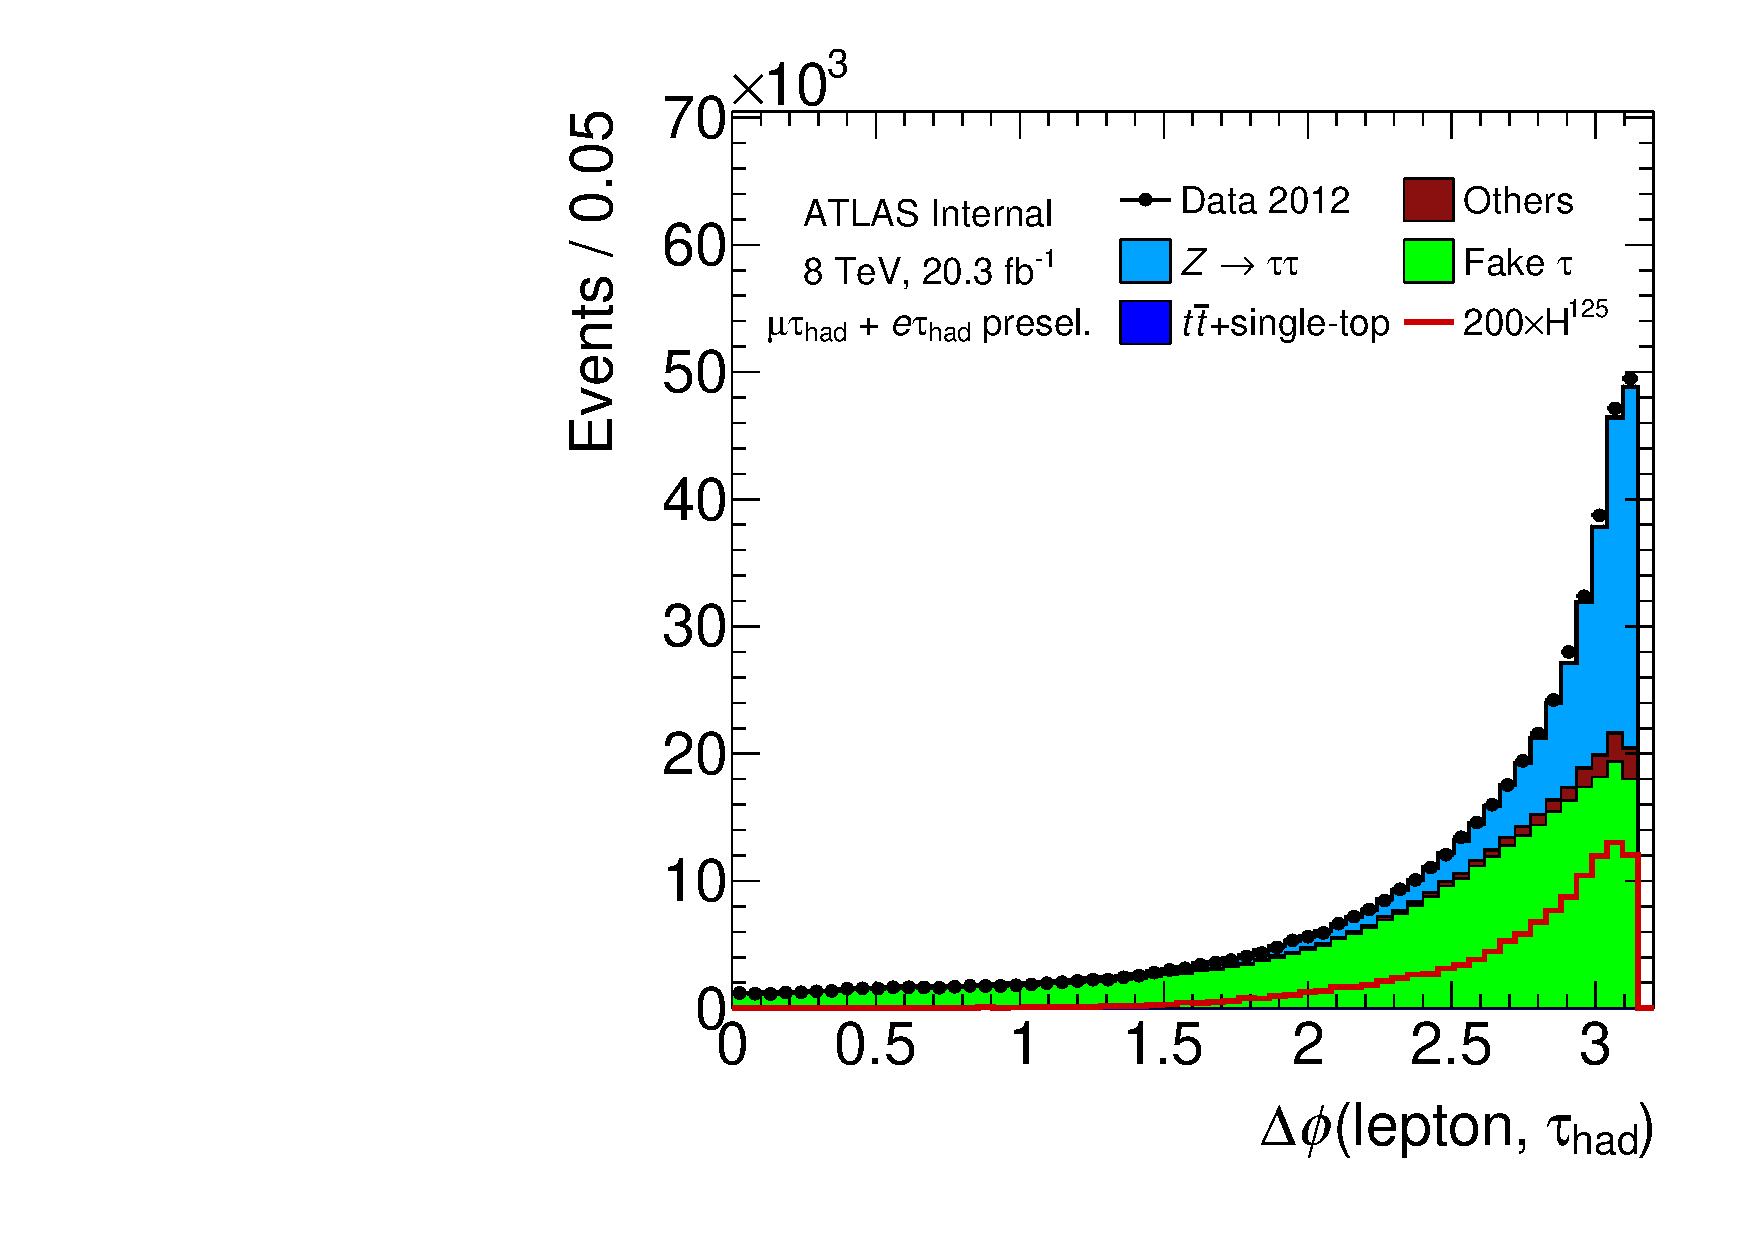
\includegraphics[width=0.32\textwidth]{figures/presel/taulep-dphi}
  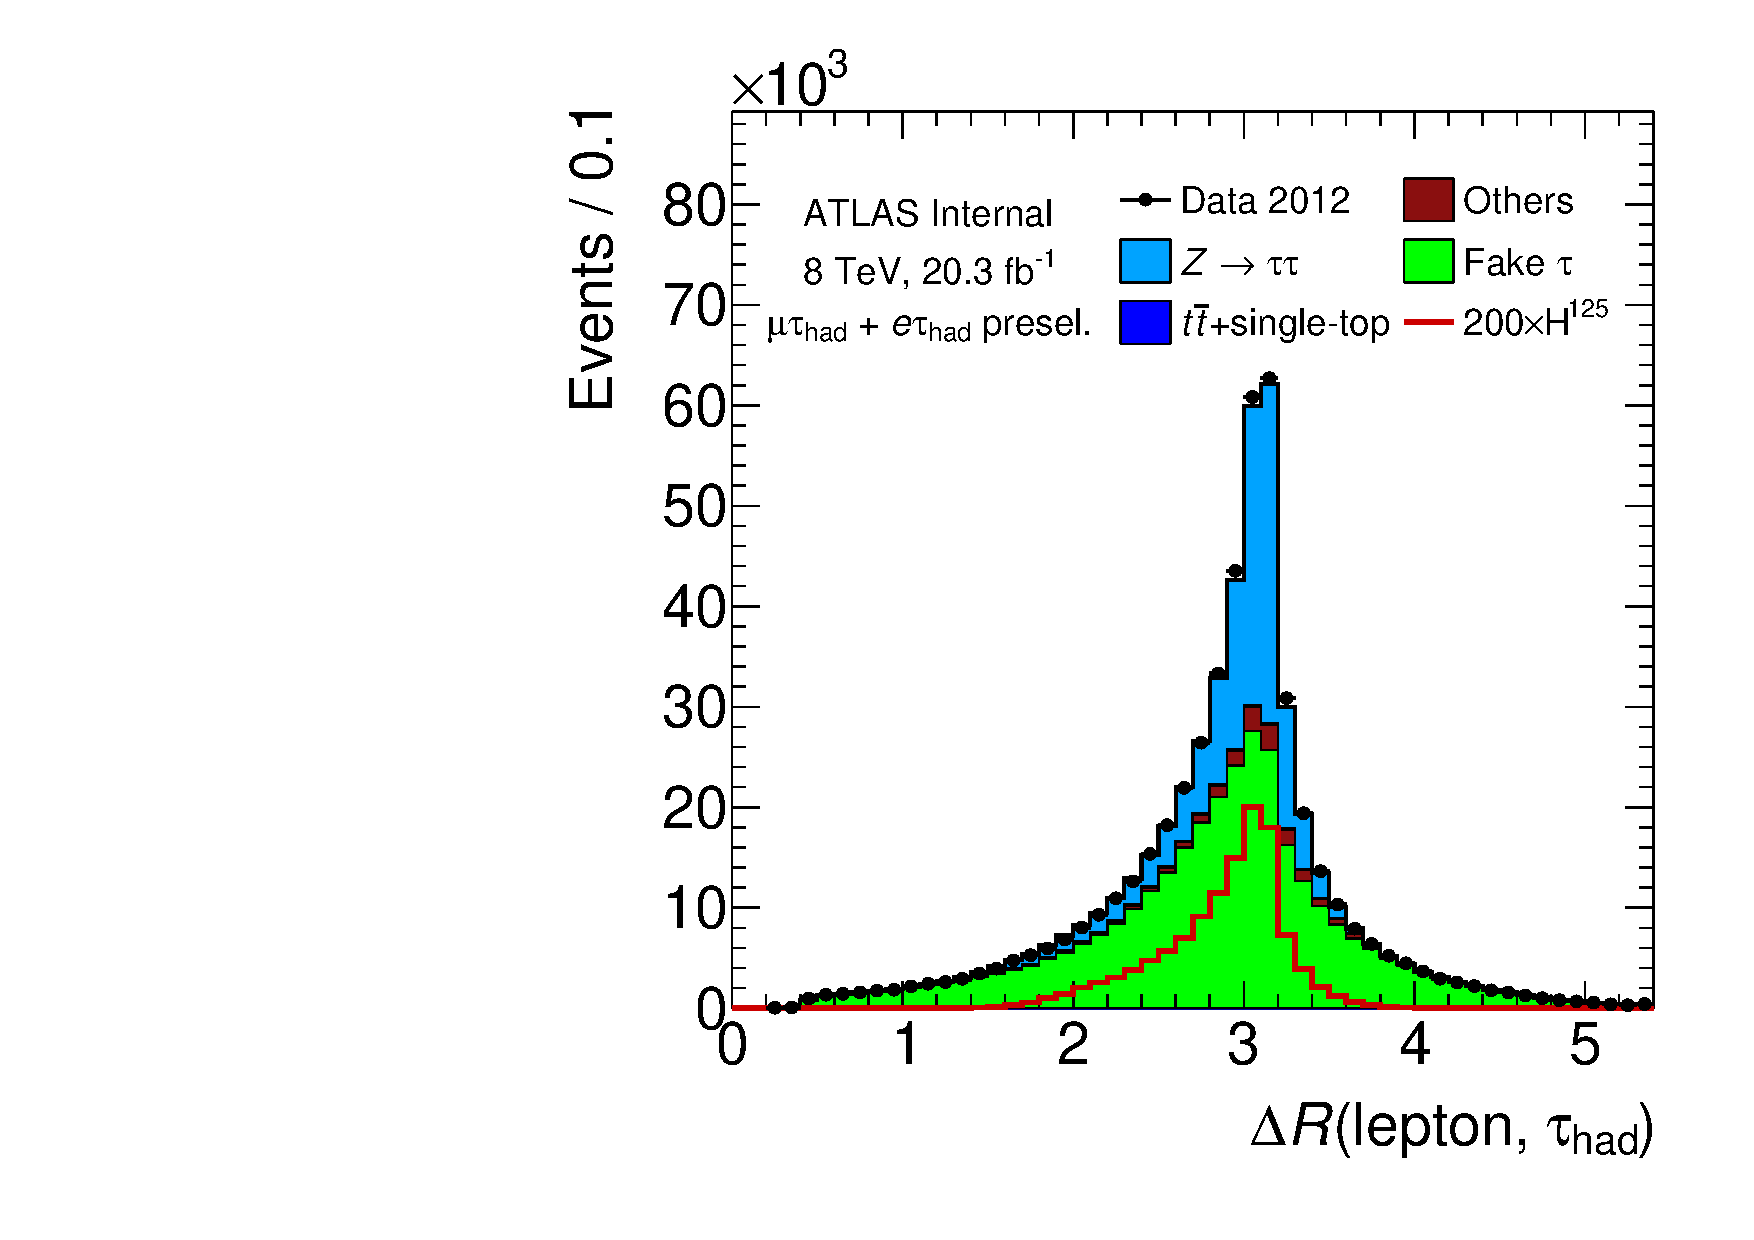
\includegraphics[width=0.32\textwidth]{figures/presel/taulep-dR}
  \caption{Variables.}
  \label{fig:stategy-presel-1}
\end{figure}

\clearpage
\begin{figure}[tp]
  \centering
  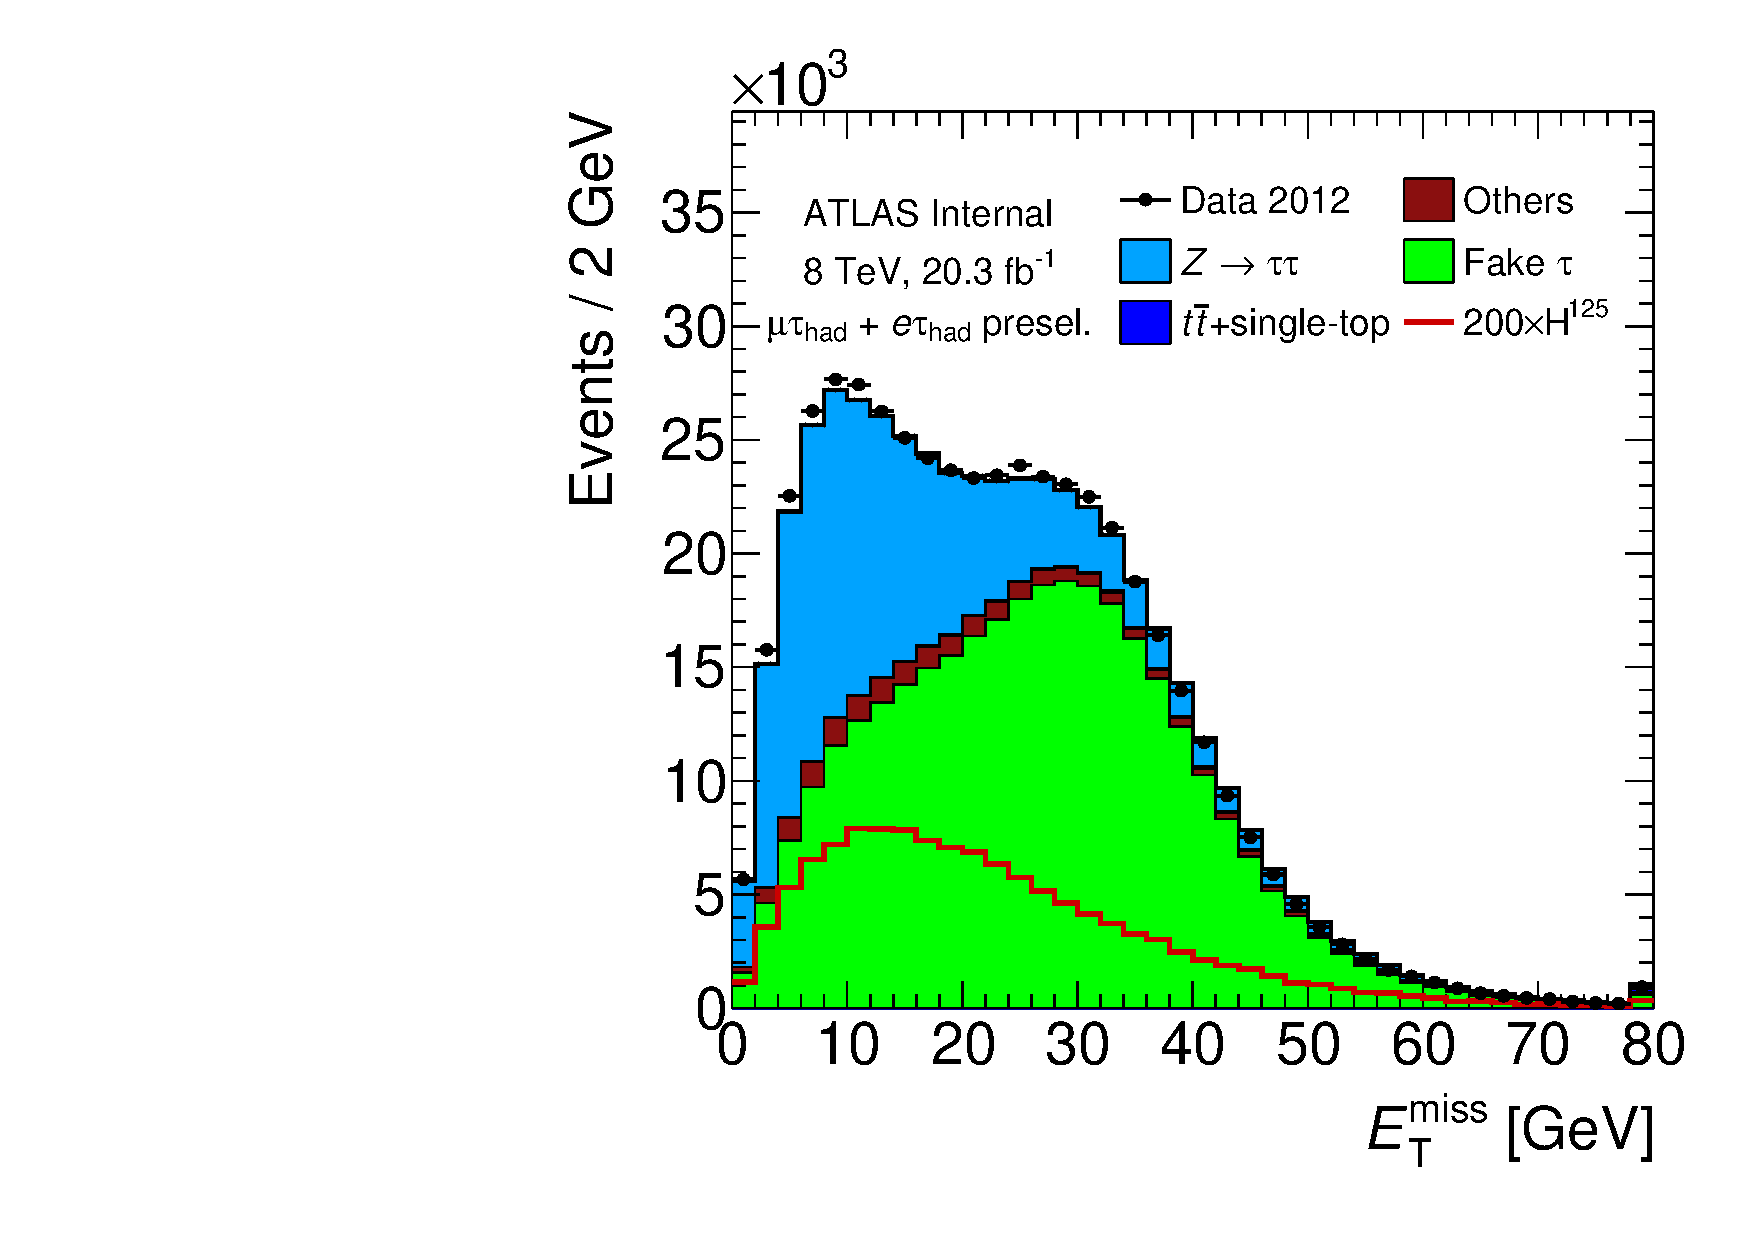
\includegraphics[width=0.32\textwidth]{figures/presel/met-pt}
  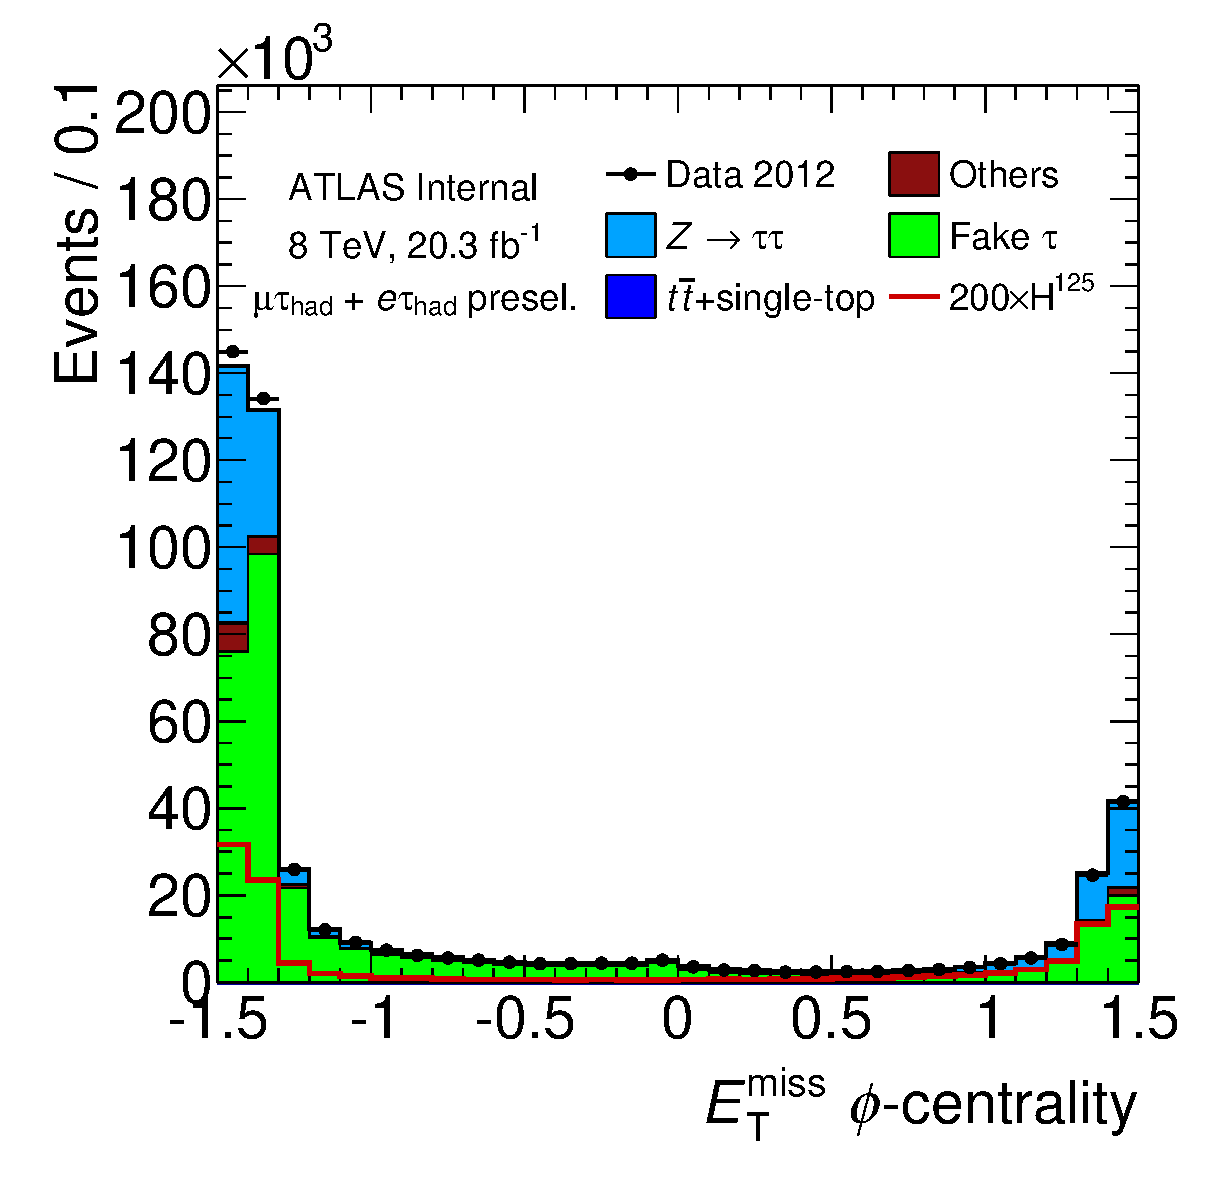
\includegraphics[width=0.32\textwidth]{figures/presel/met-phi-centrality}
  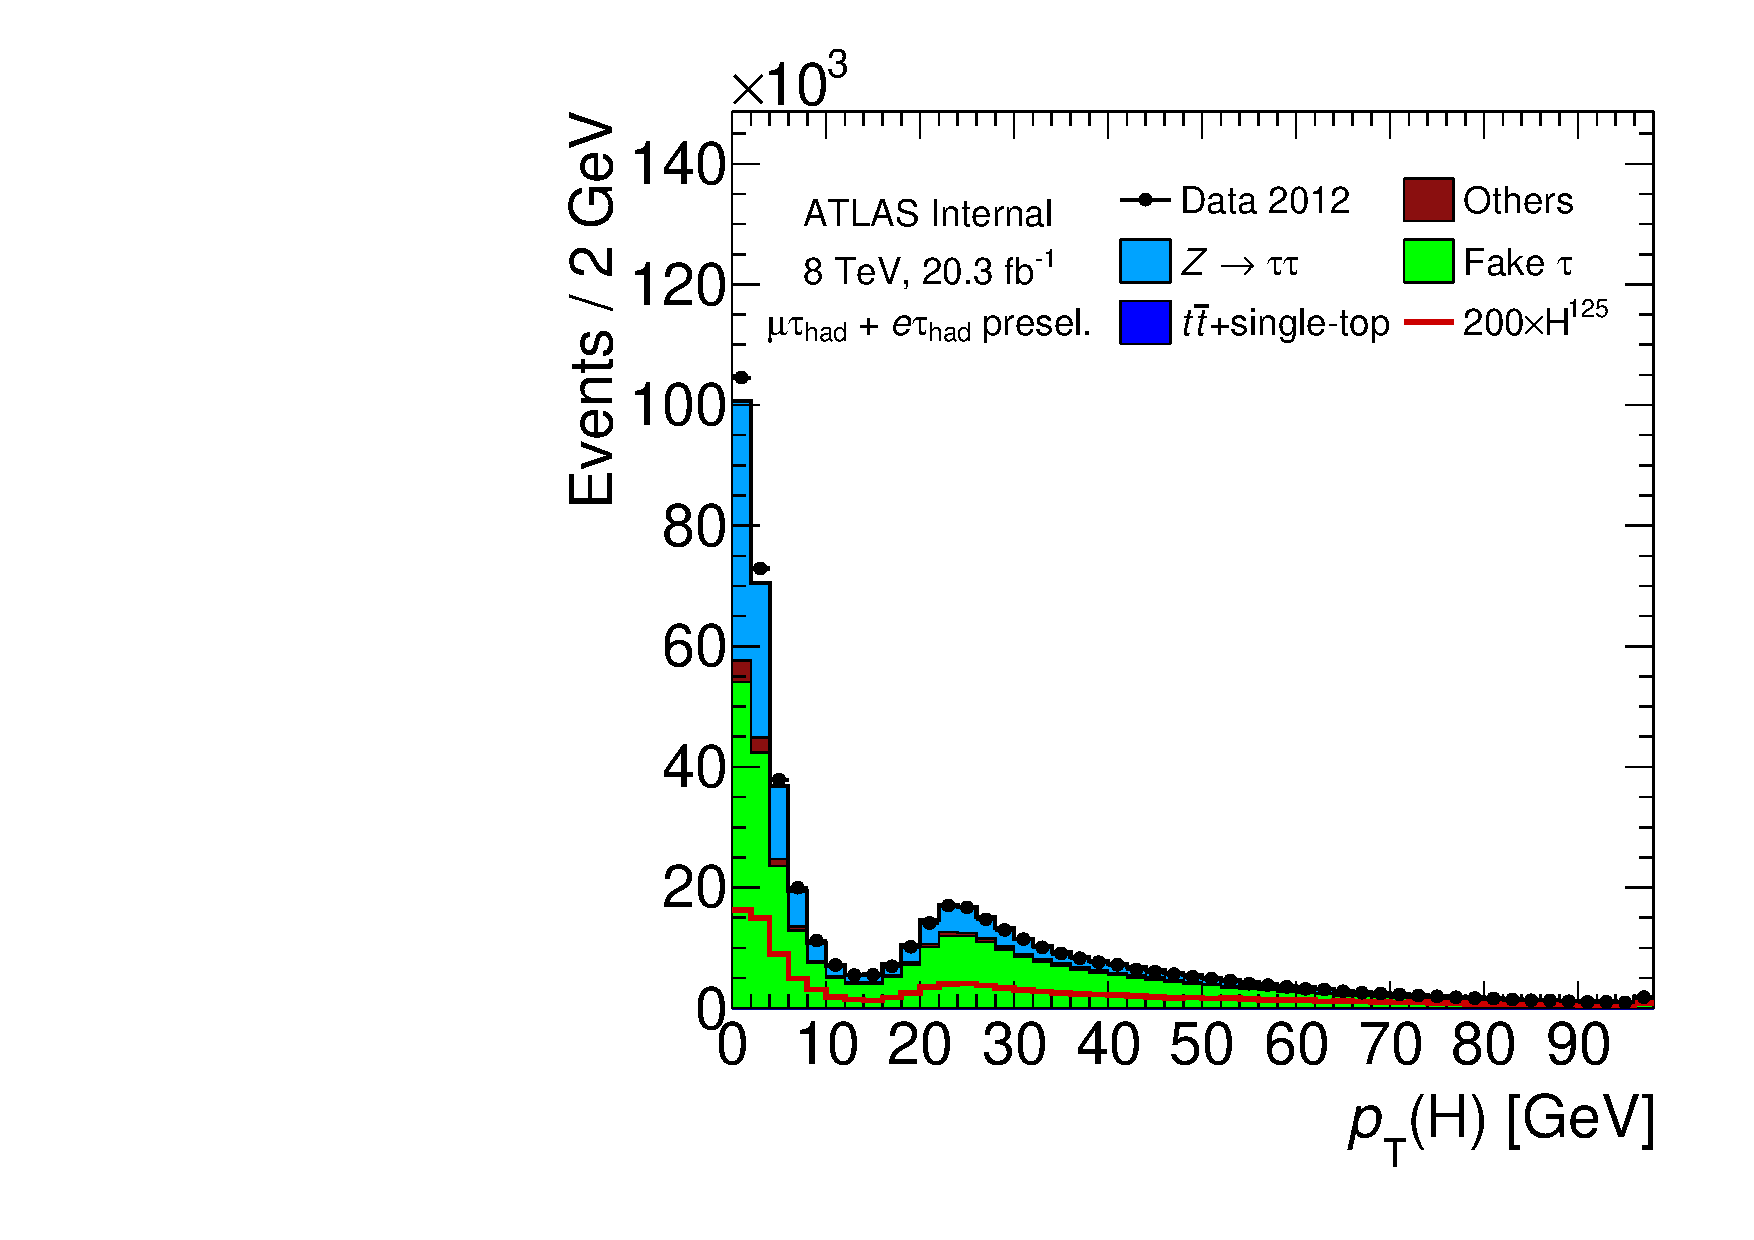
\includegraphics[width=0.32\textwidth]{figures/presel/H-pt}
  % --------------
  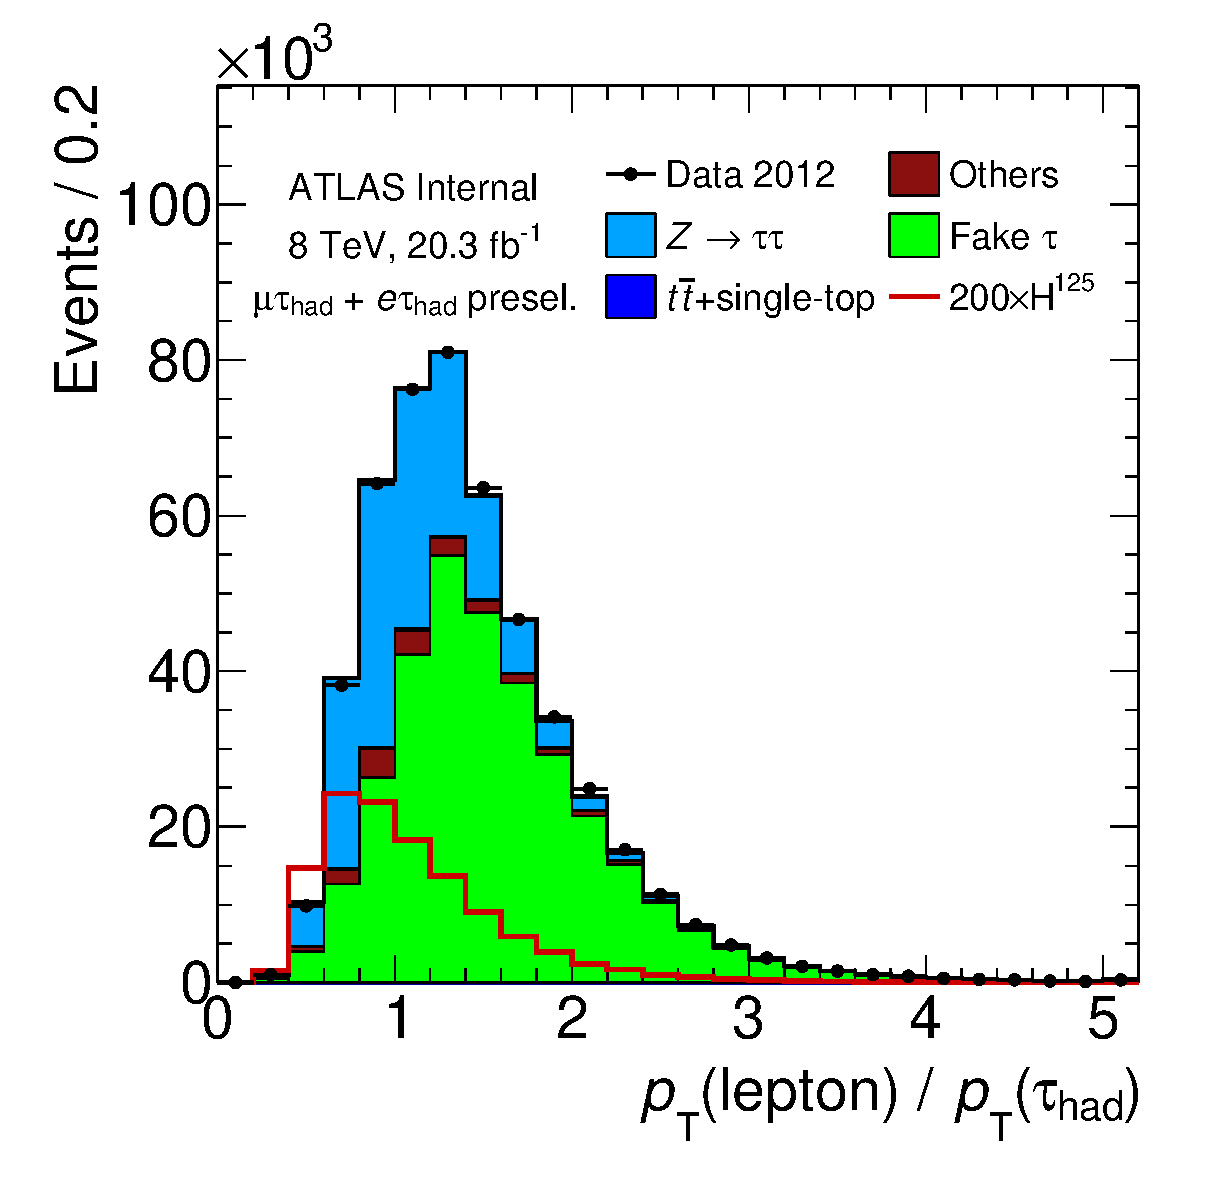
\includegraphics[width=0.32\textwidth]{figures/presel/taulep-ptratio}
  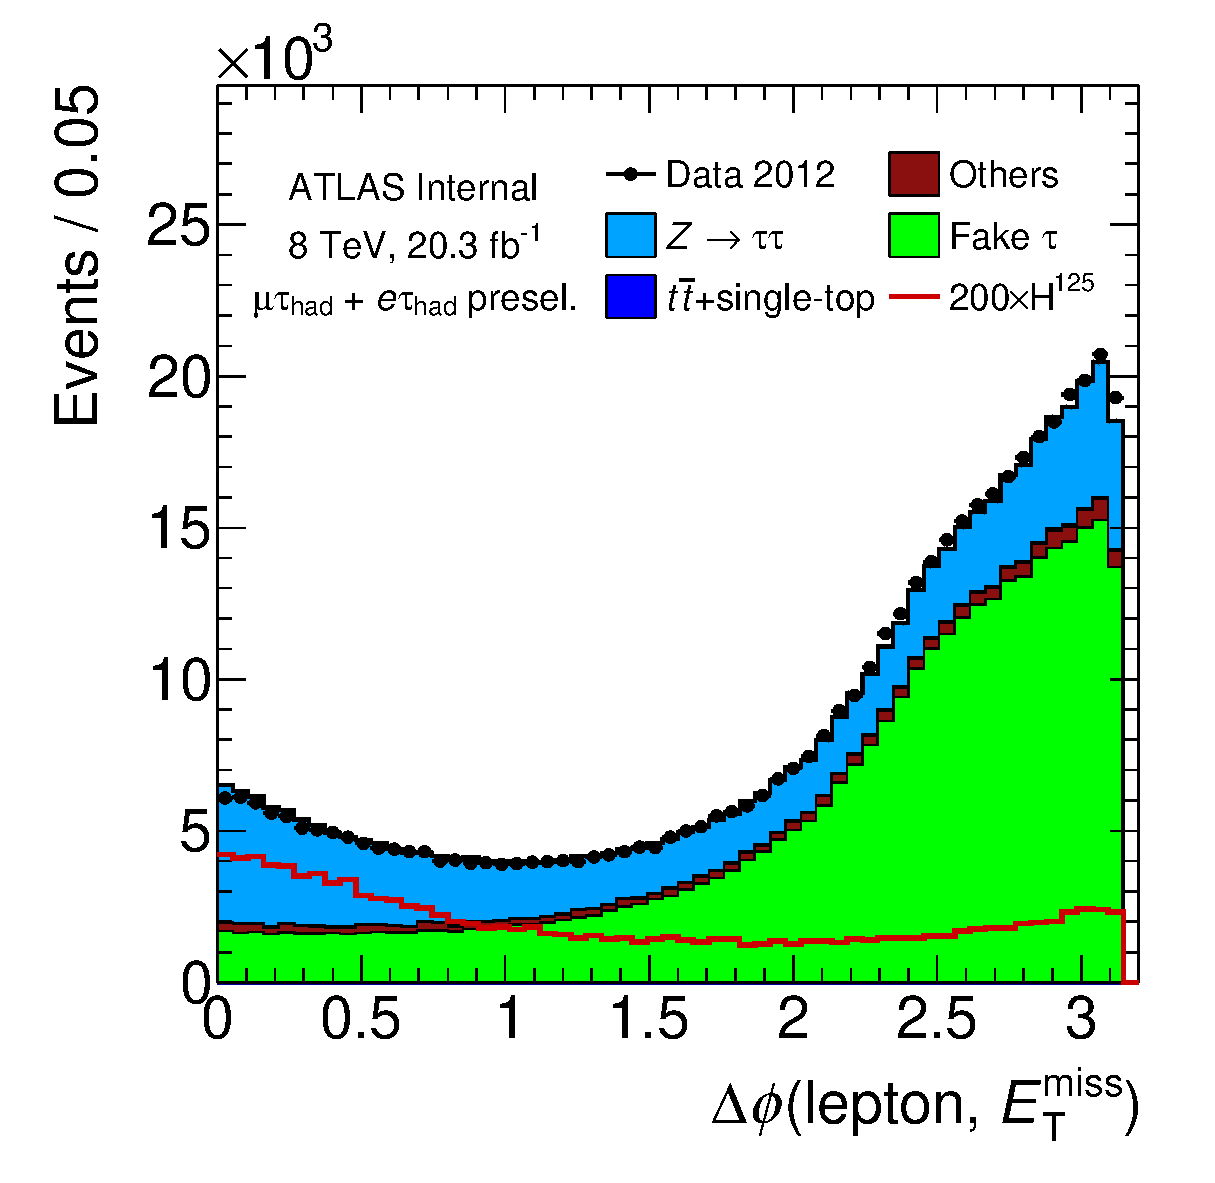
\includegraphics[width=0.32\textwidth]{figures/presel/lepmet-dphi}
  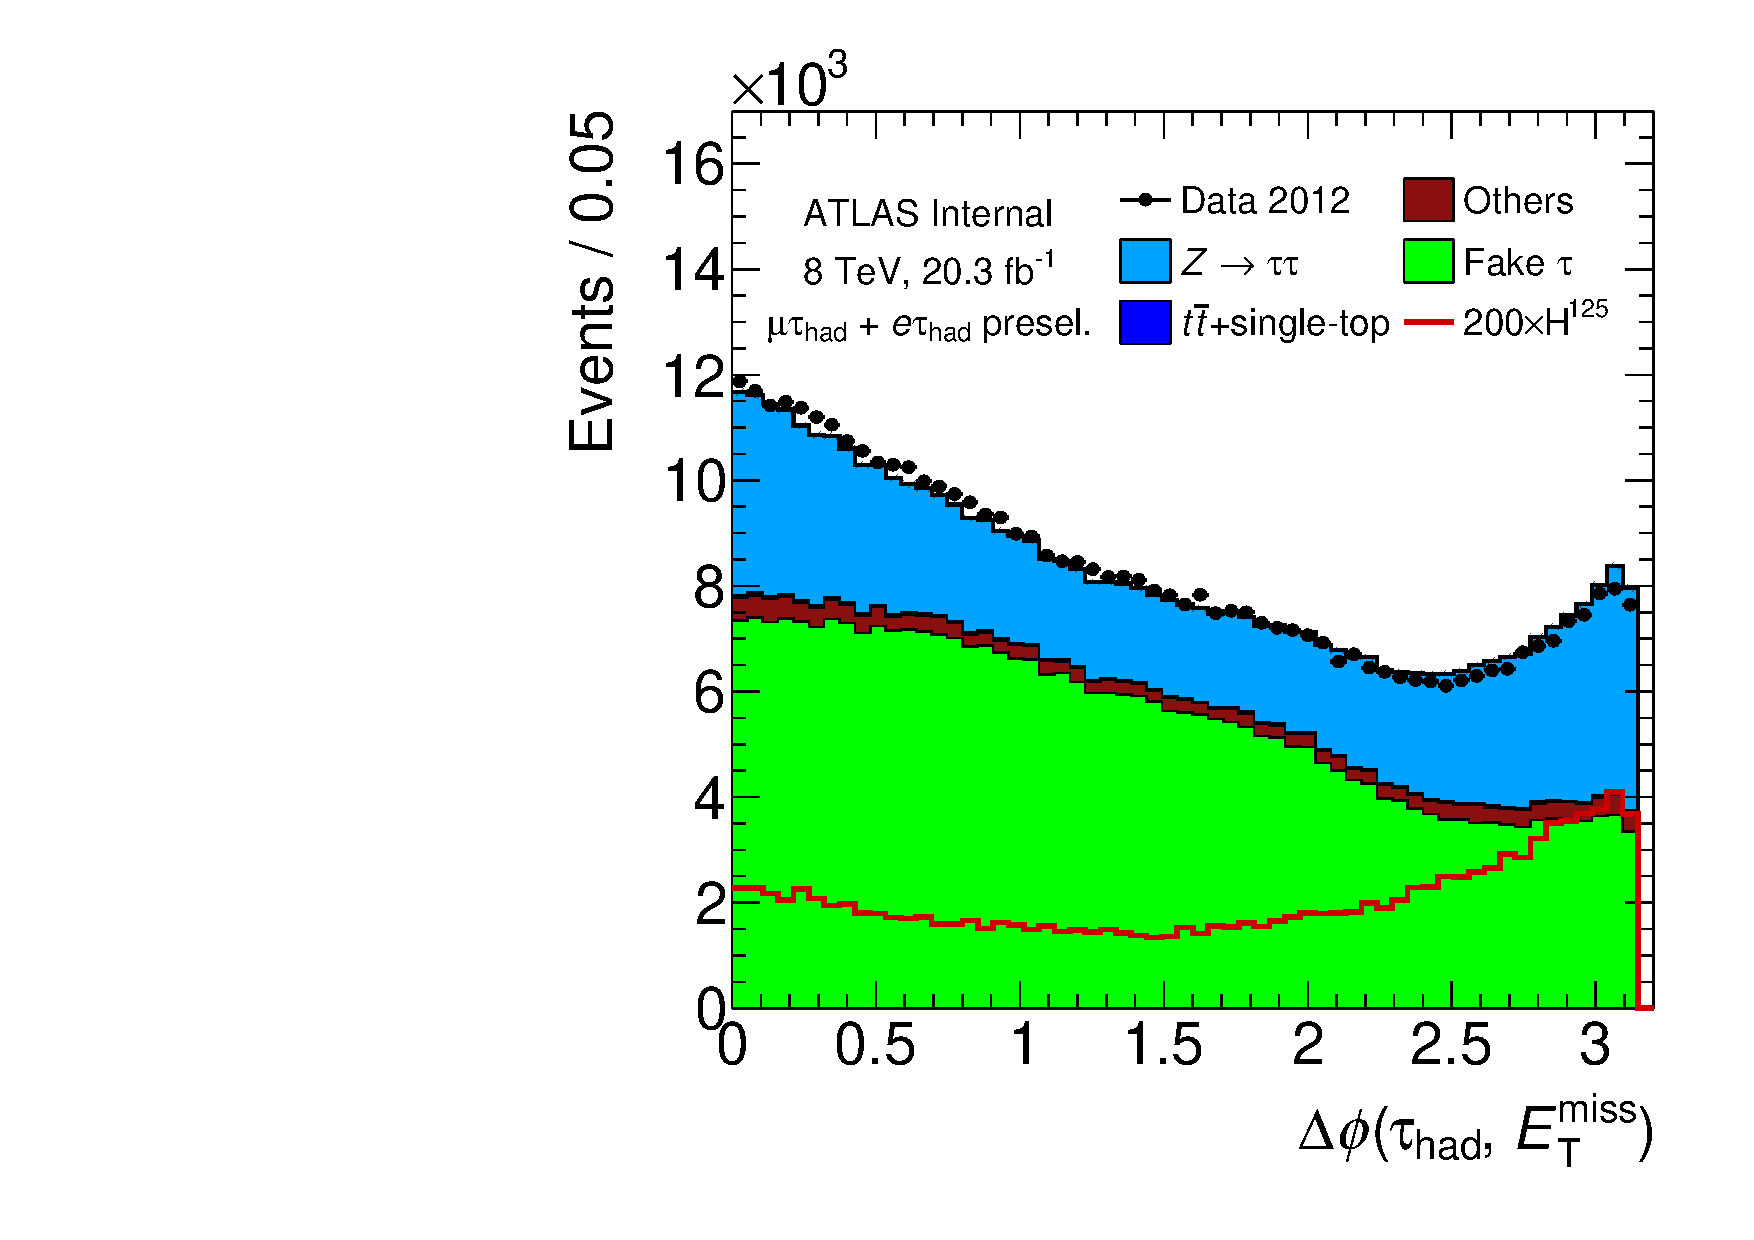
\includegraphics[width=0.32\textwidth]{figures/presel/taumet-dphi}
  % --------------
  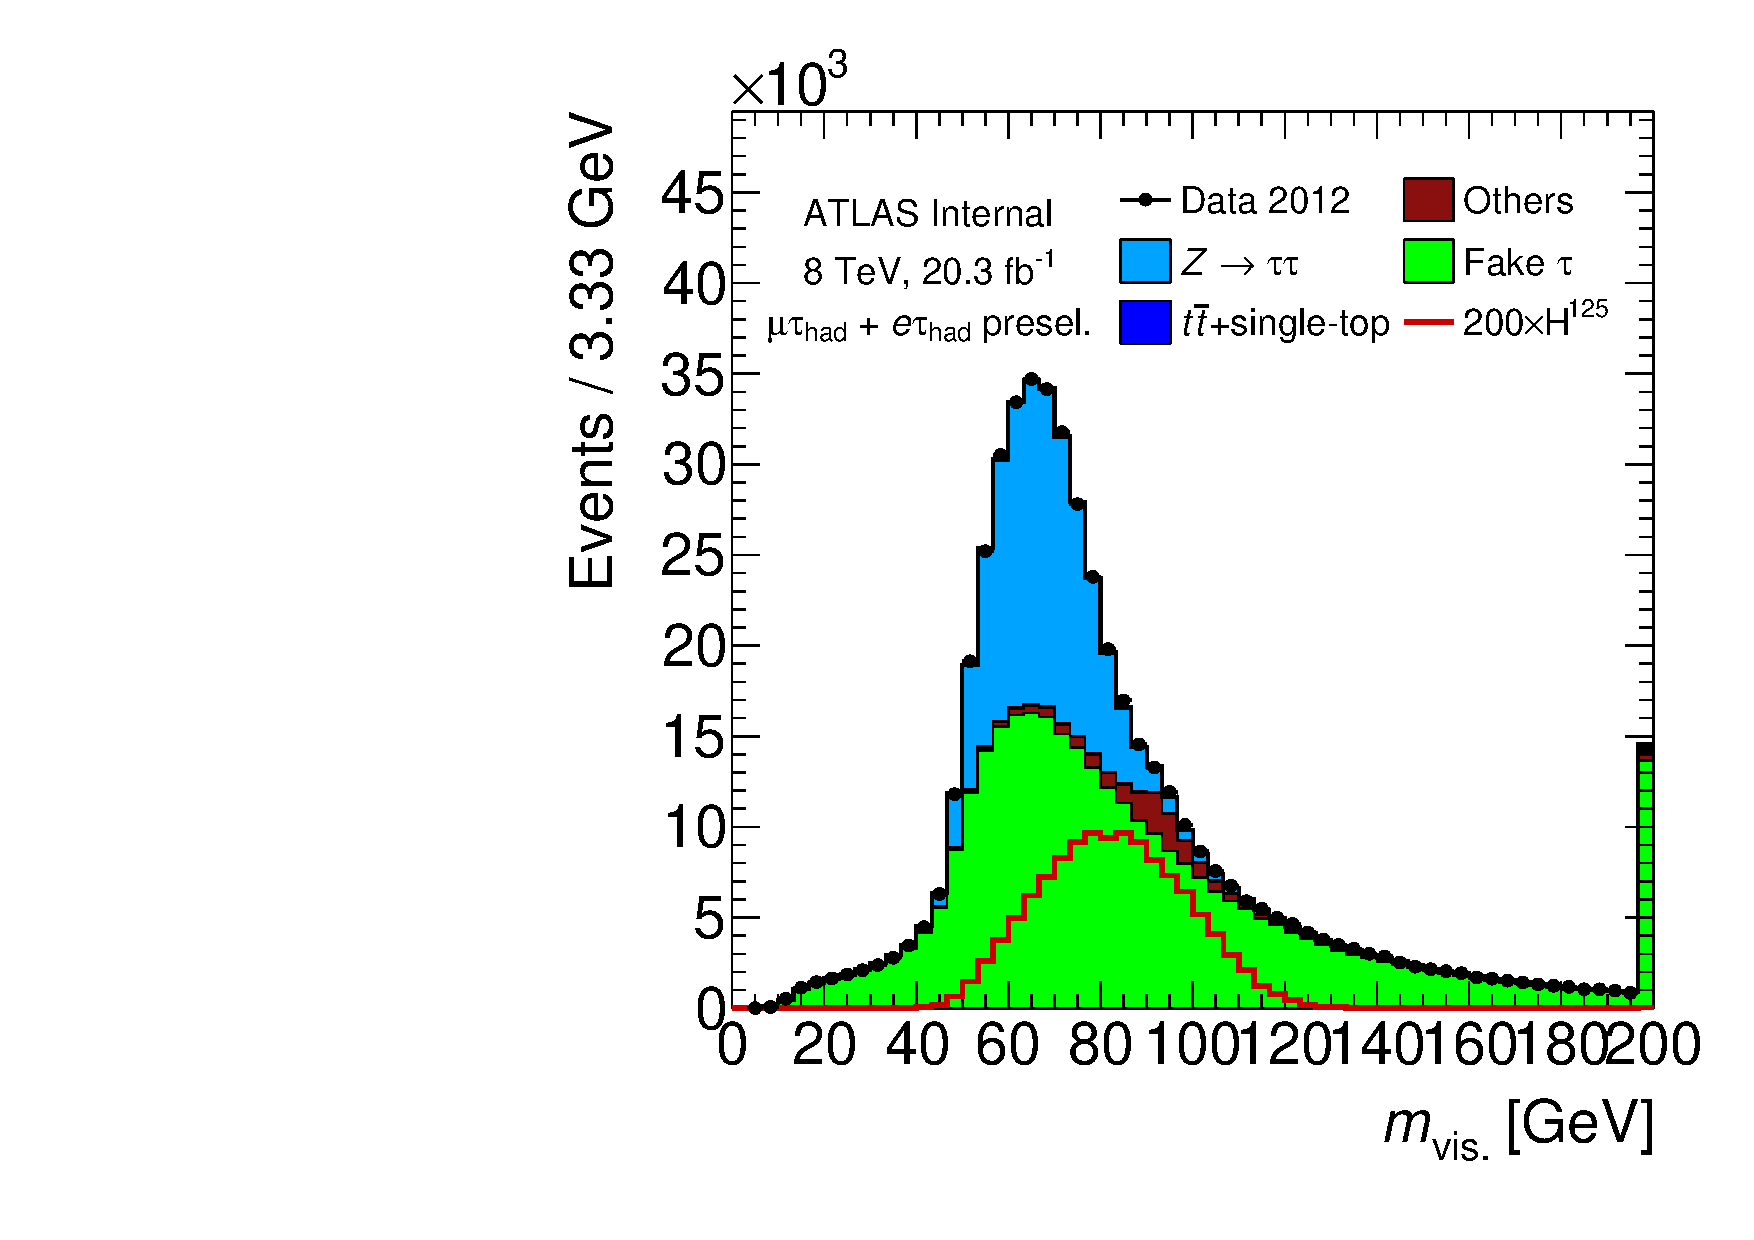
\includegraphics[width=0.32\textwidth]{figures/presel/mvis}
  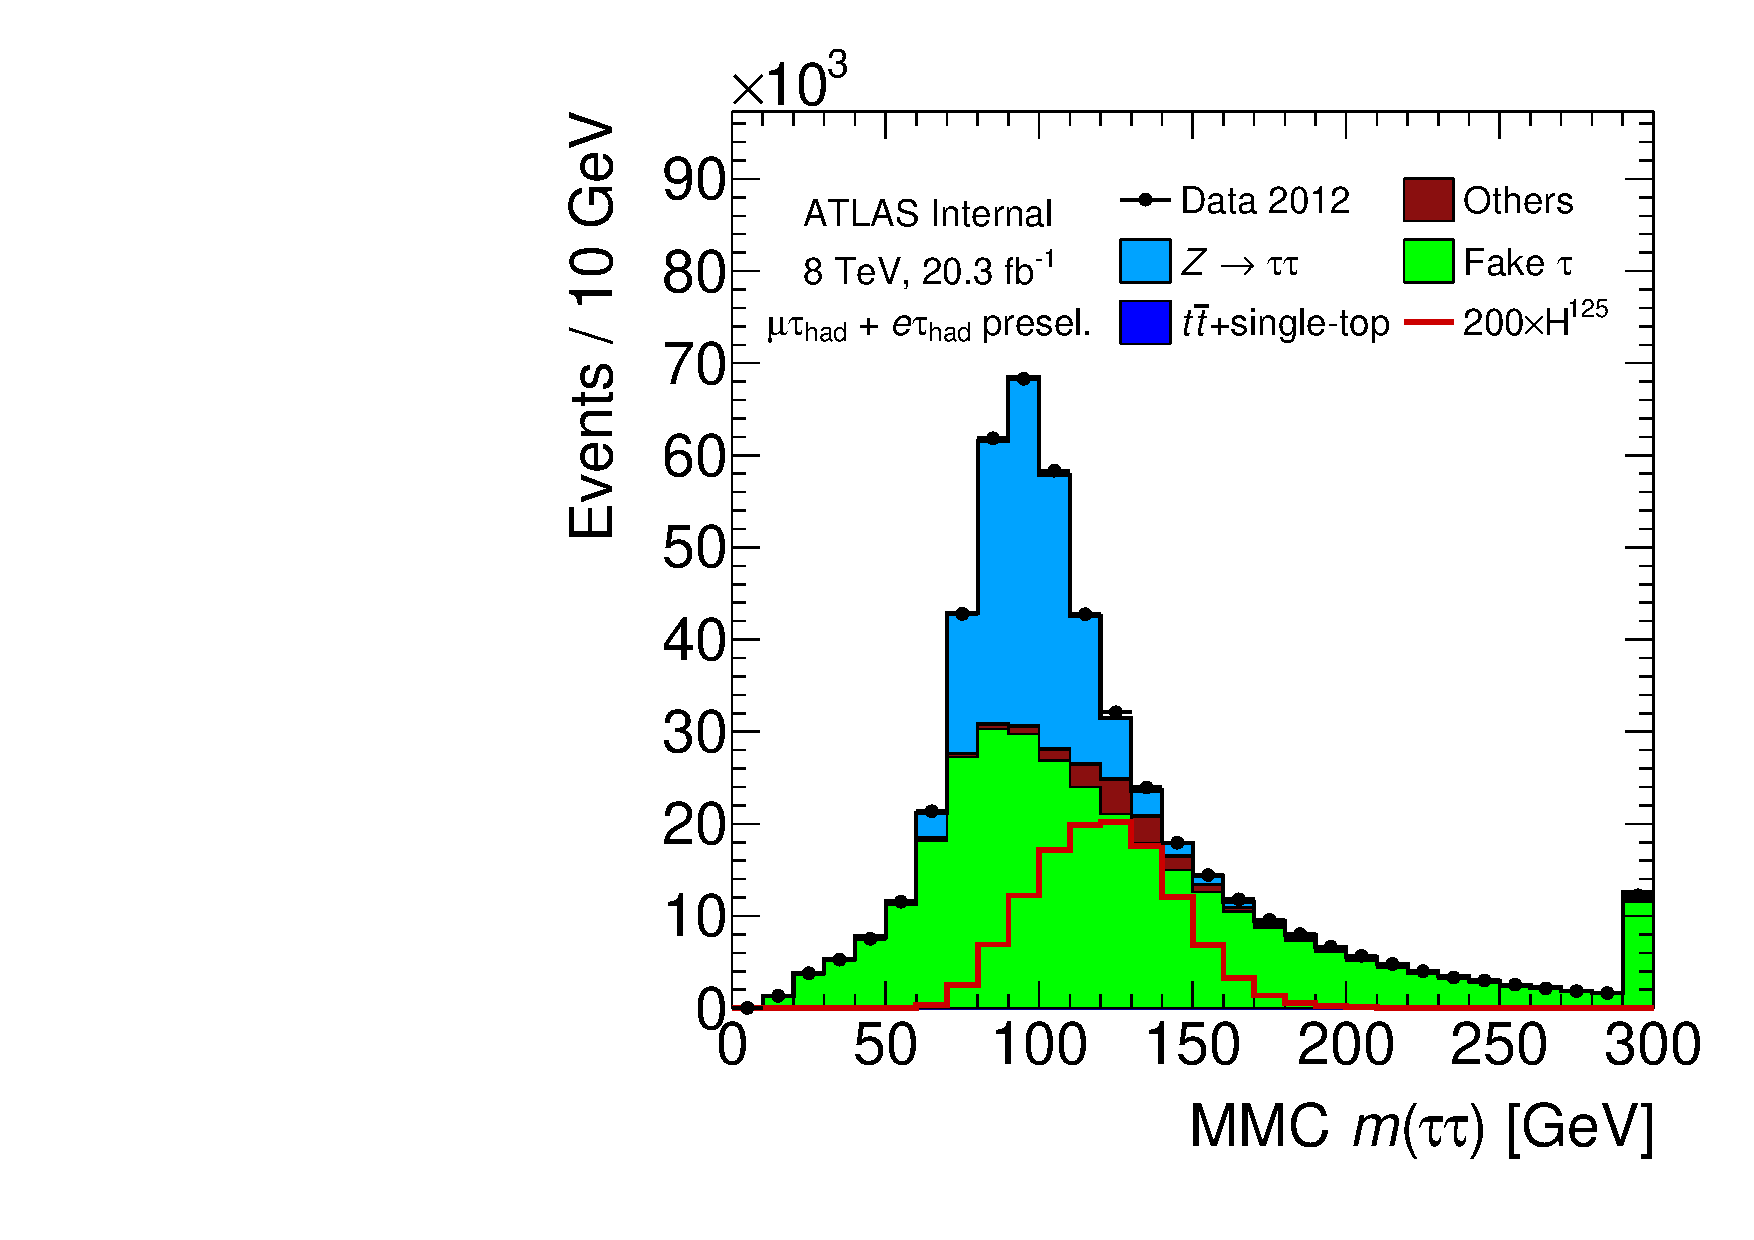
\includegraphics[width=0.32\textwidth]{figures/presel/mMMC}
  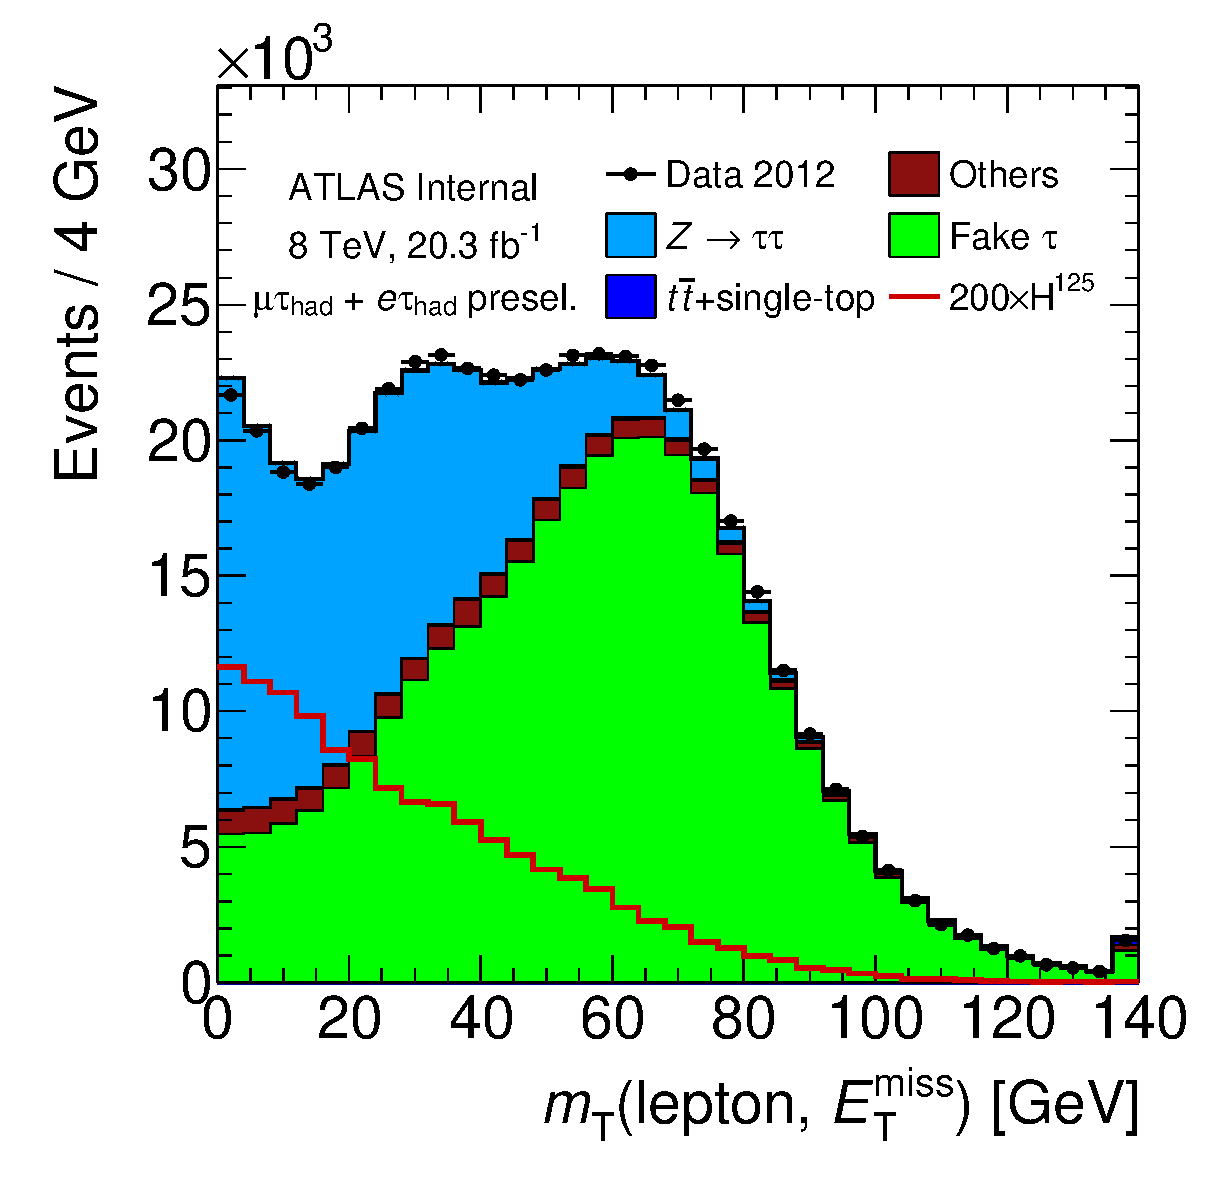
\includegraphics[width=0.32\textwidth]{figures/presel/mT-hi}
  % --------------
  \caption{Variables.}
  \label{fig:stategy-presel-2}
\end{figure}

\clearpage
\section{$\tautau$ mass reconstruction}
\label{sec:strategy-mtautau}

% MMC cartoon
% ---------------------------------------------------------------------------------
\begin{figure}[tp]
  \centering
  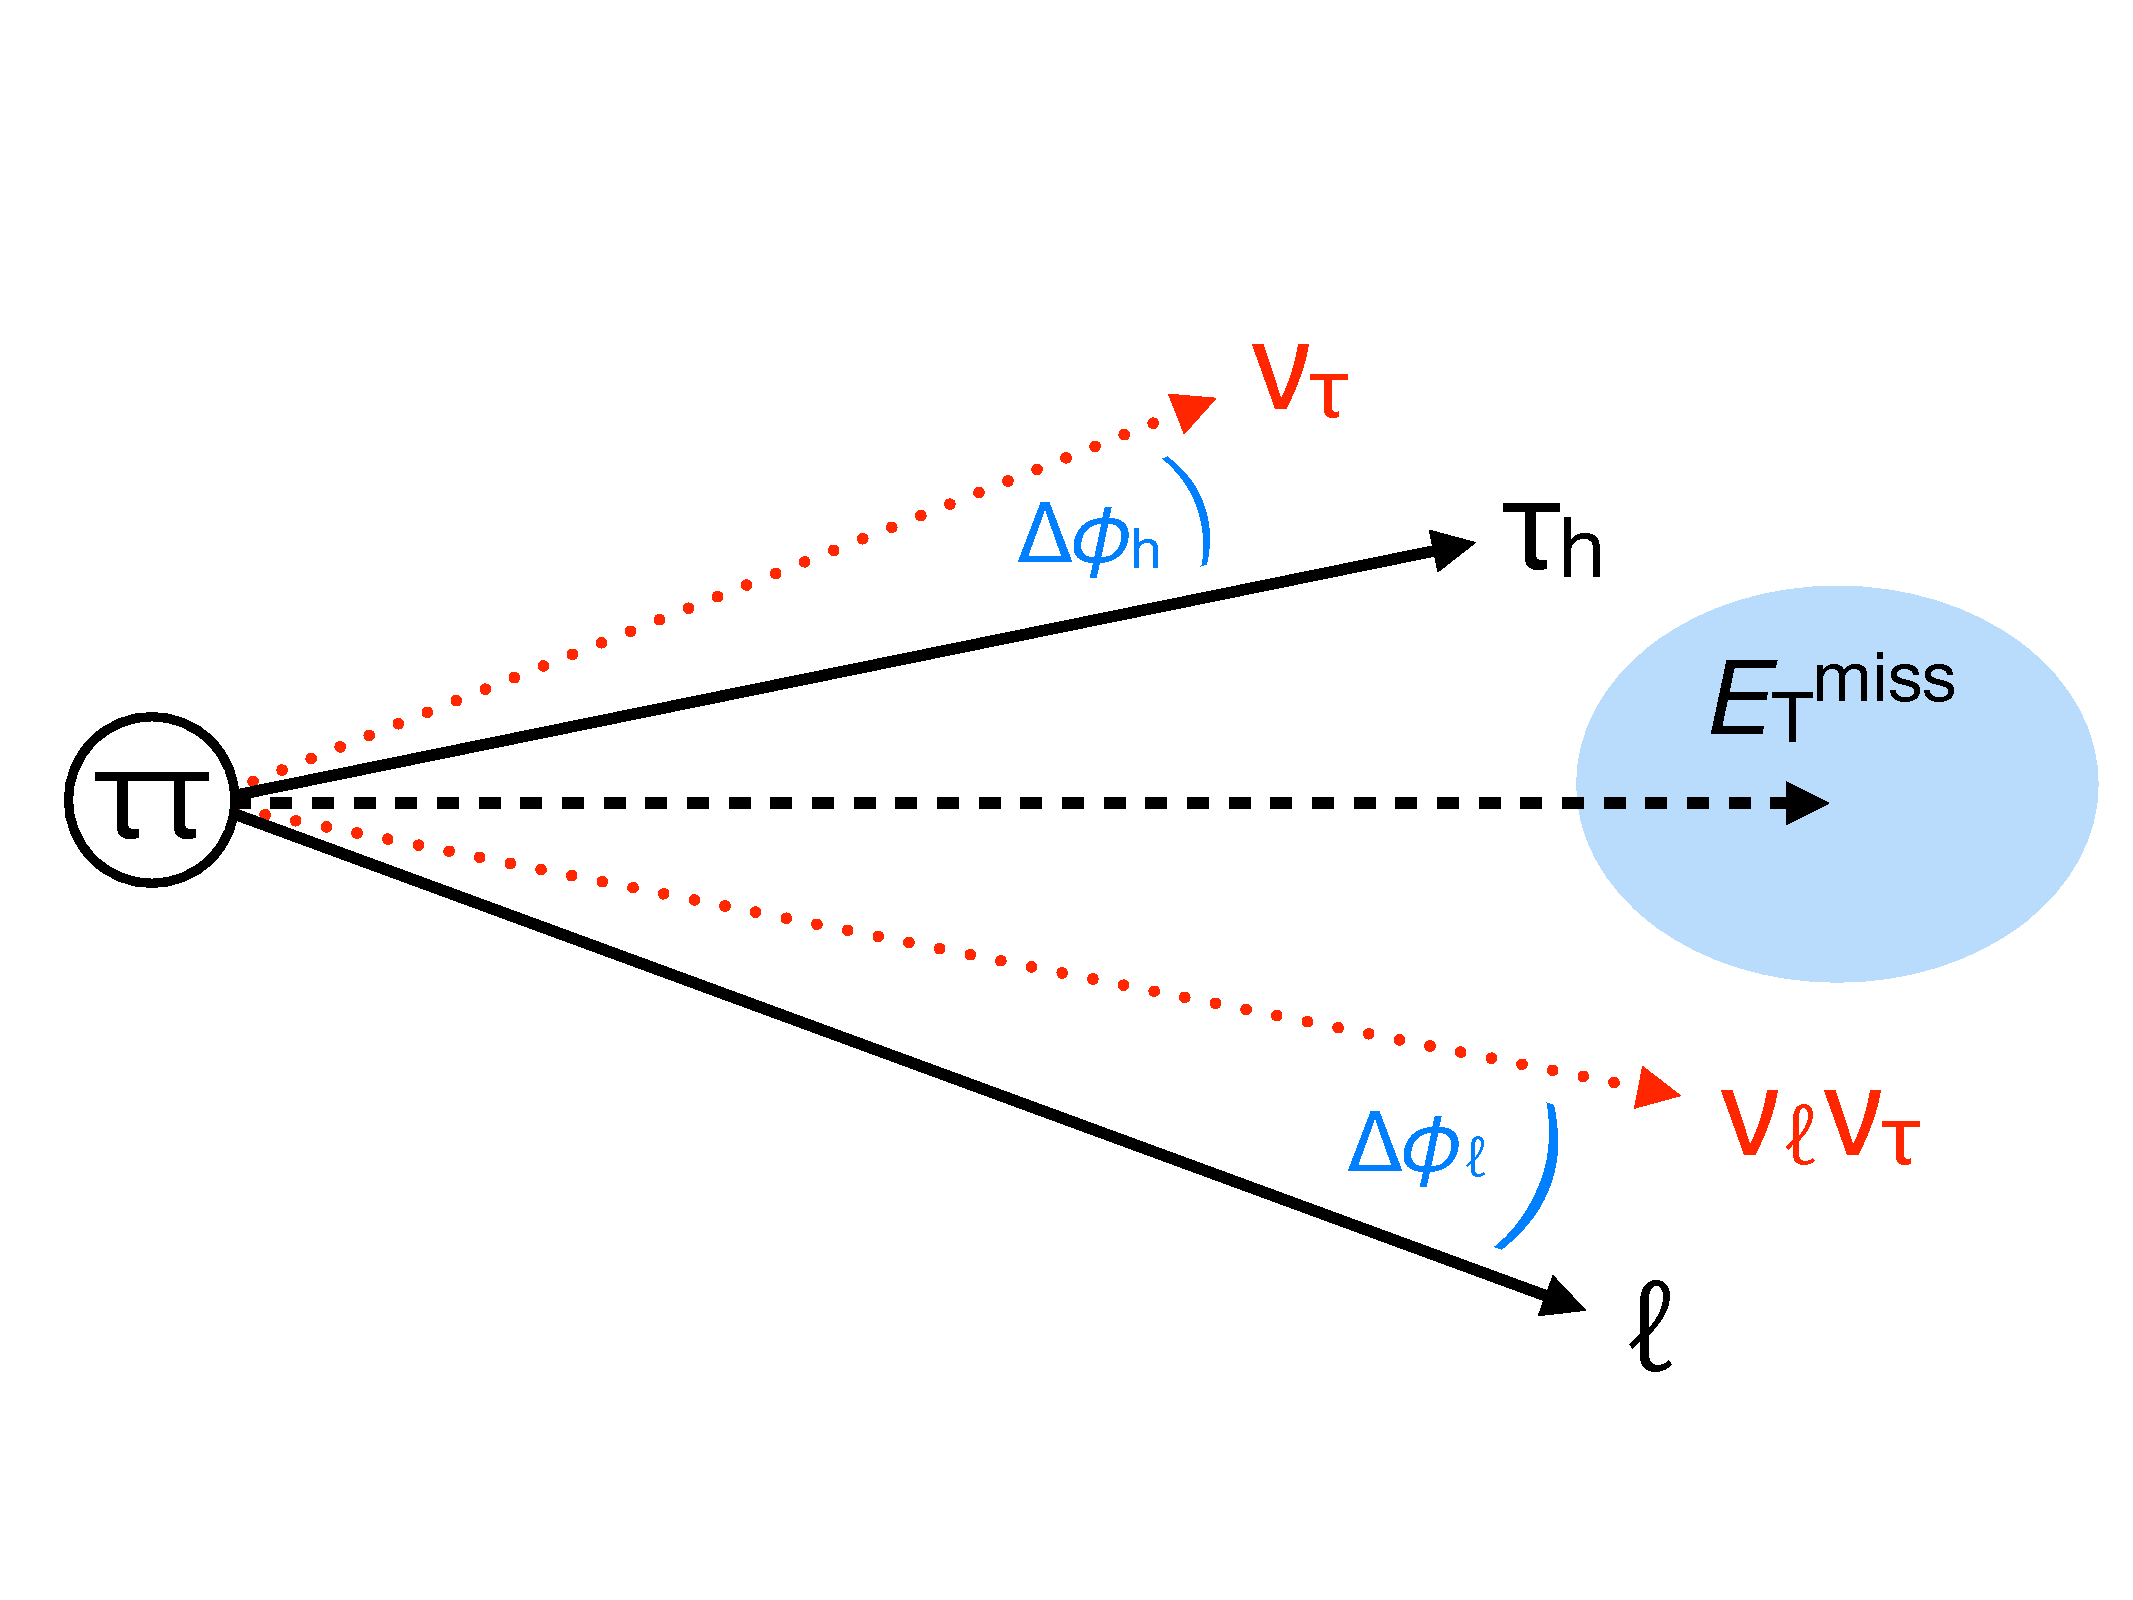
\includegraphics[width=0.90\textwidth]{figures/mtautau/mmc-cartoon}
  \caption{Variables.}
  \label{fig:strategy-mtautau-cartoon}
\end{figure}

% MMC input assumptions
% ---------------------------------------------------------------------------------
\begin{figure}[tp]
  \centering
  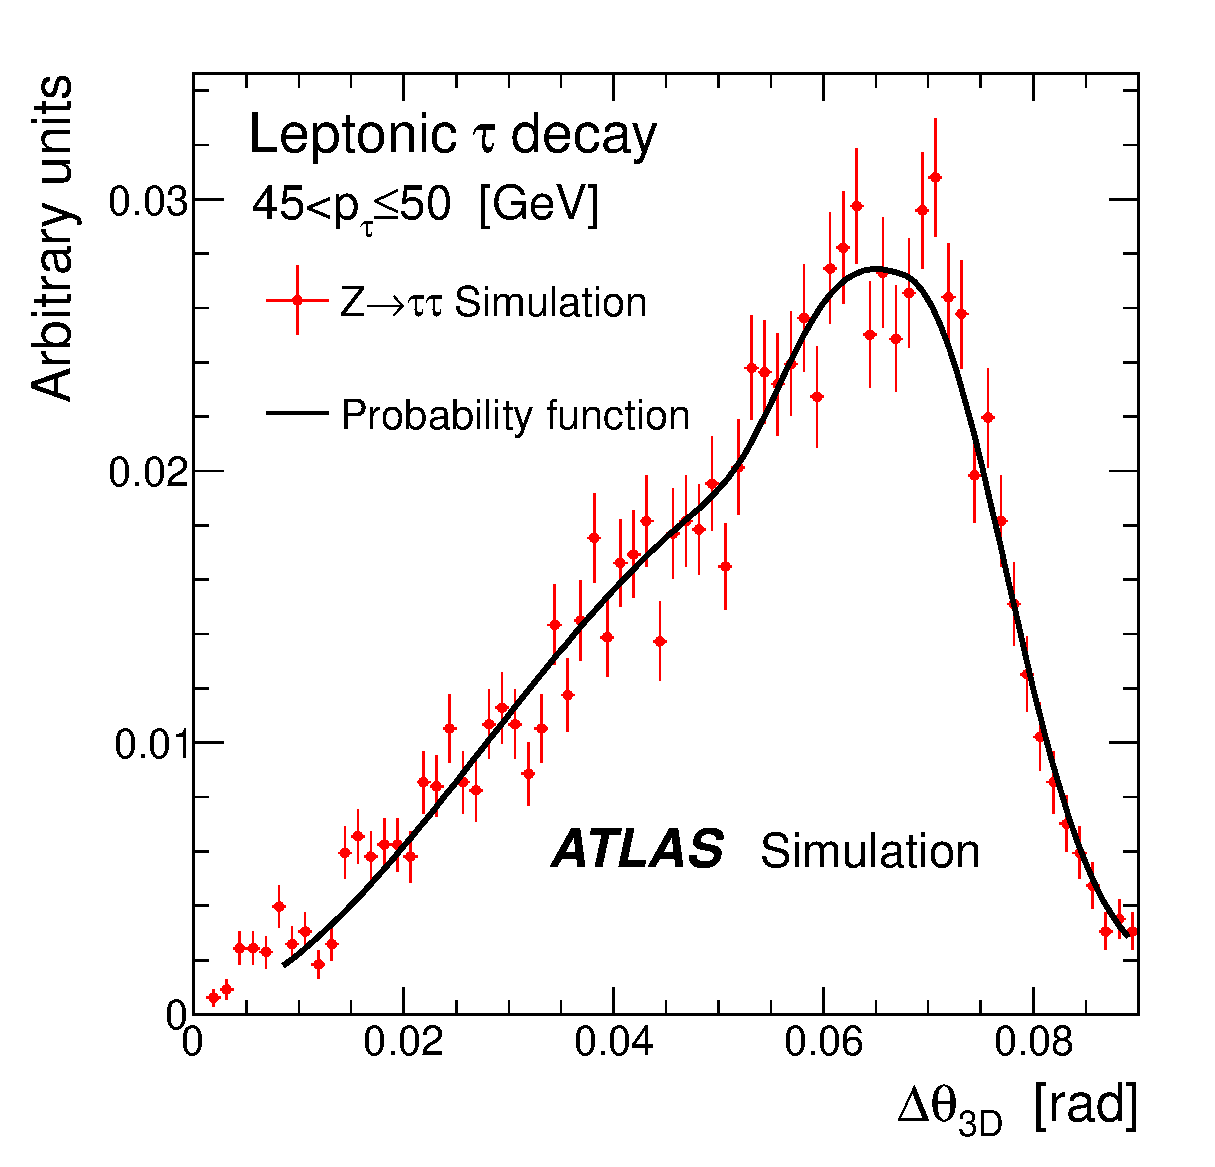
\includegraphics[width=0.32\textwidth]{figures/ATLAS-CONF-2011-132/fig_01a}
  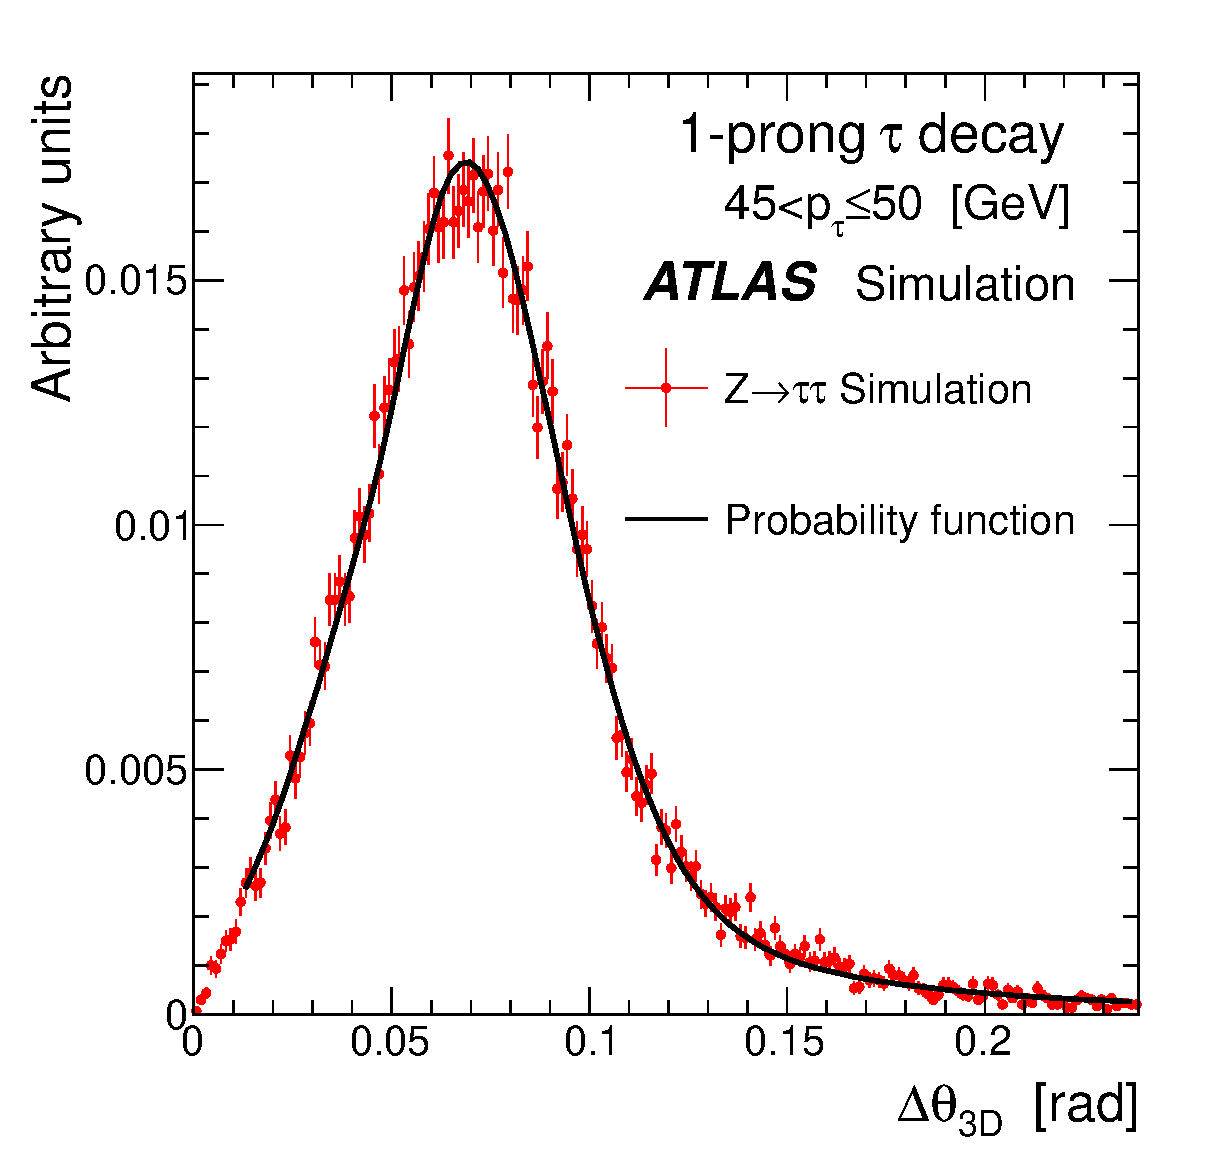
\includegraphics[width=0.32\textwidth]{figures/ATLAS-CONF-2011-132/fig_01b}
  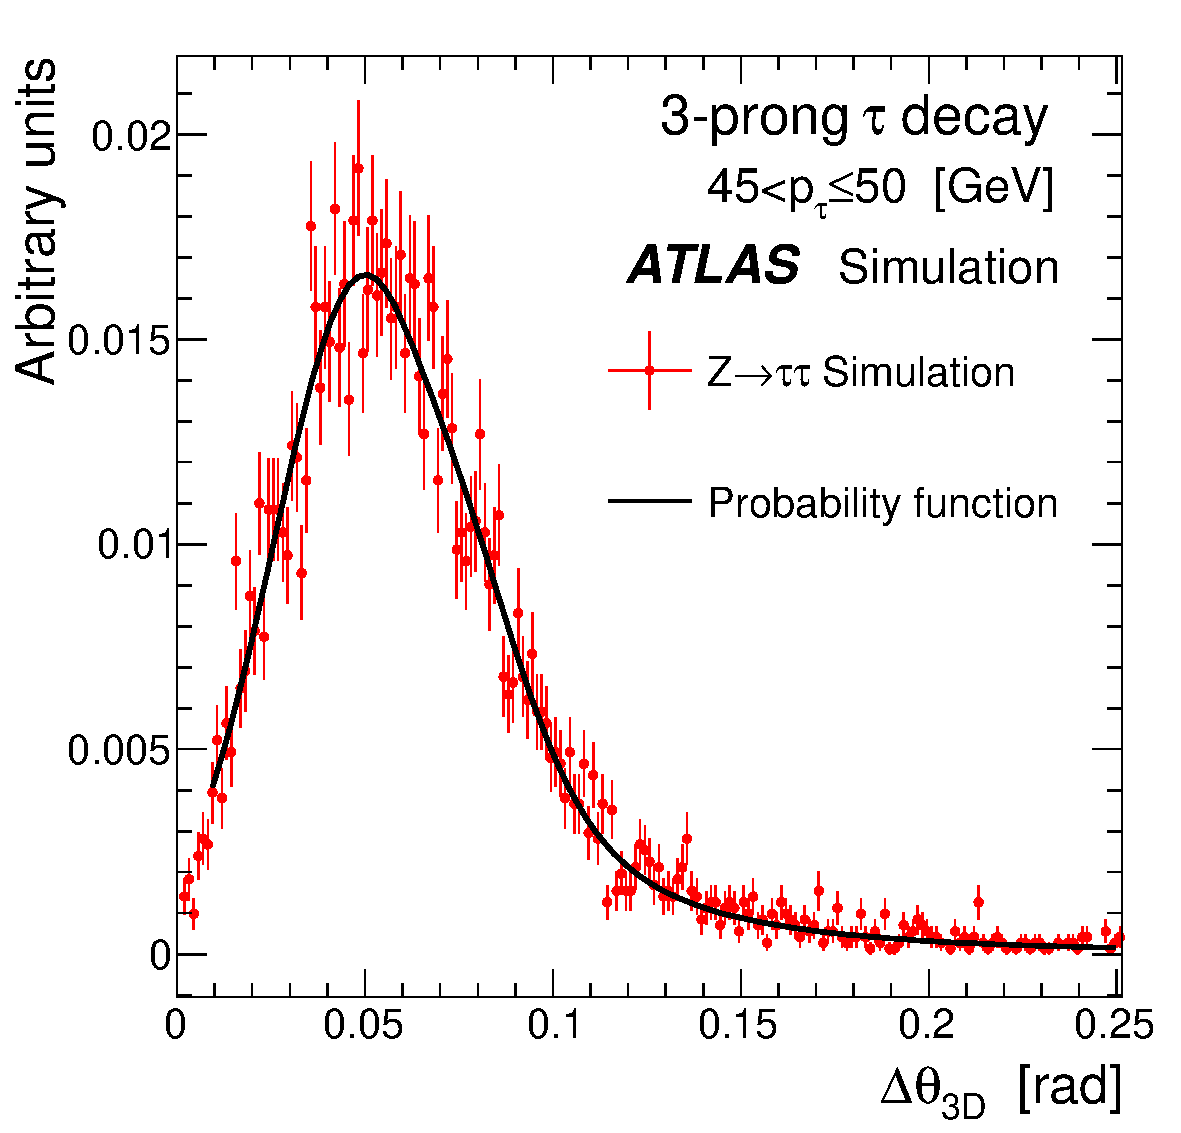
\includegraphics[width=0.32\textwidth]{figures/ATLAS-CONF-2011-132/fig_01c}
  \caption{Variables.}
  \label{fig:strategy-mtautau-inputs}
\end{figure}

% mass ROCs
% ---------------------------------------------------------------------------------
\begin{figure}[tp]
  \centering
  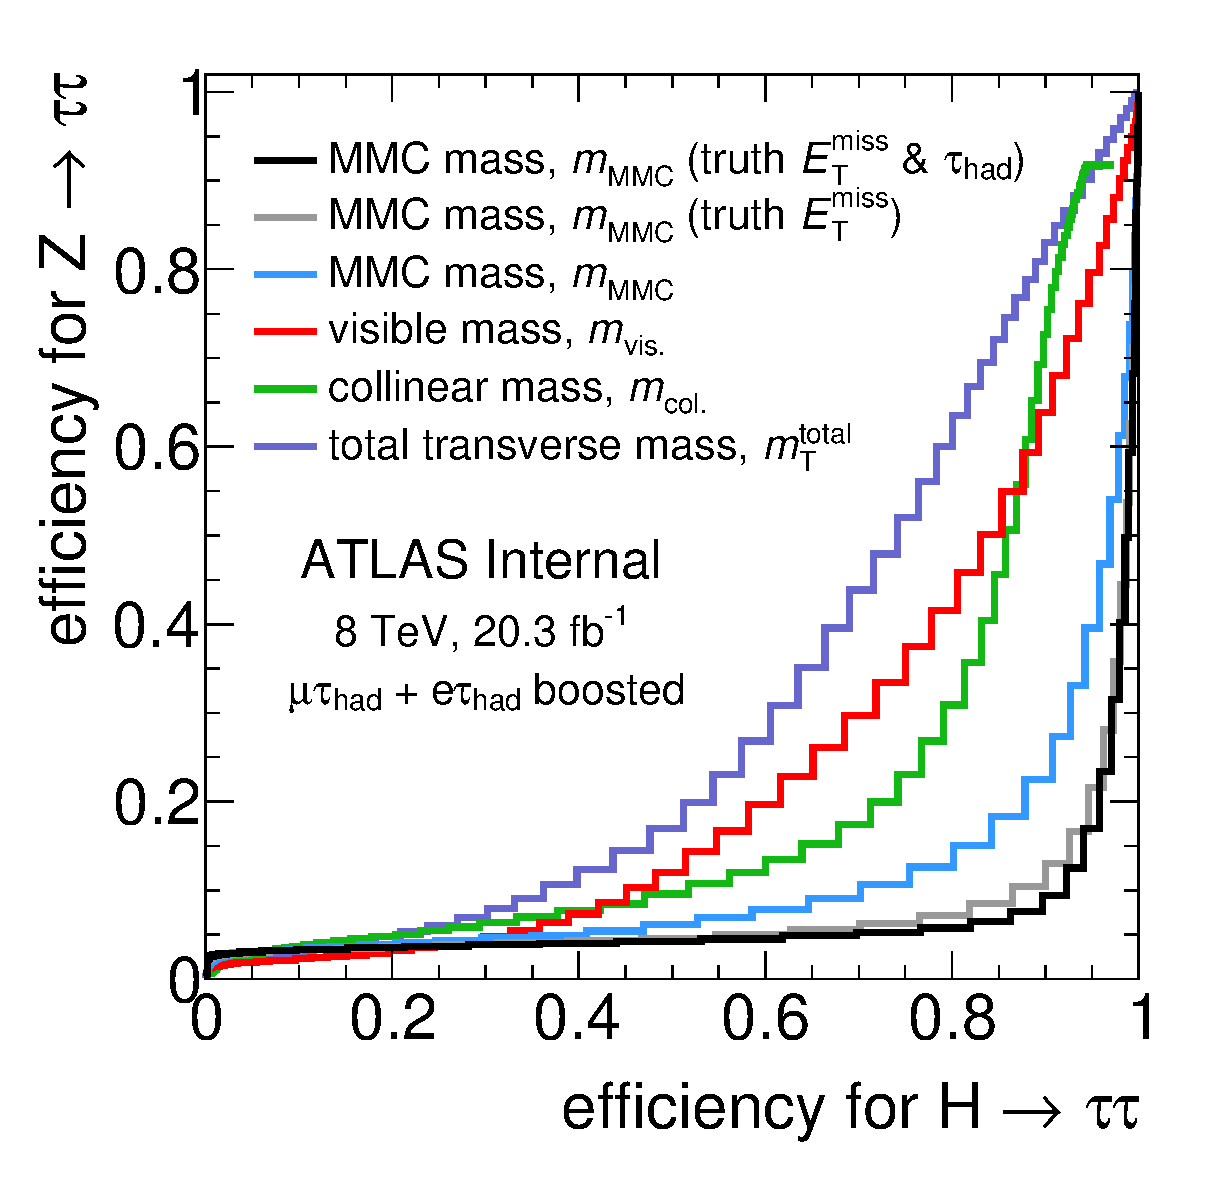
\includegraphics[width=0.48\textwidth]{figures/mtautau/mtautau-ROC-boost}
  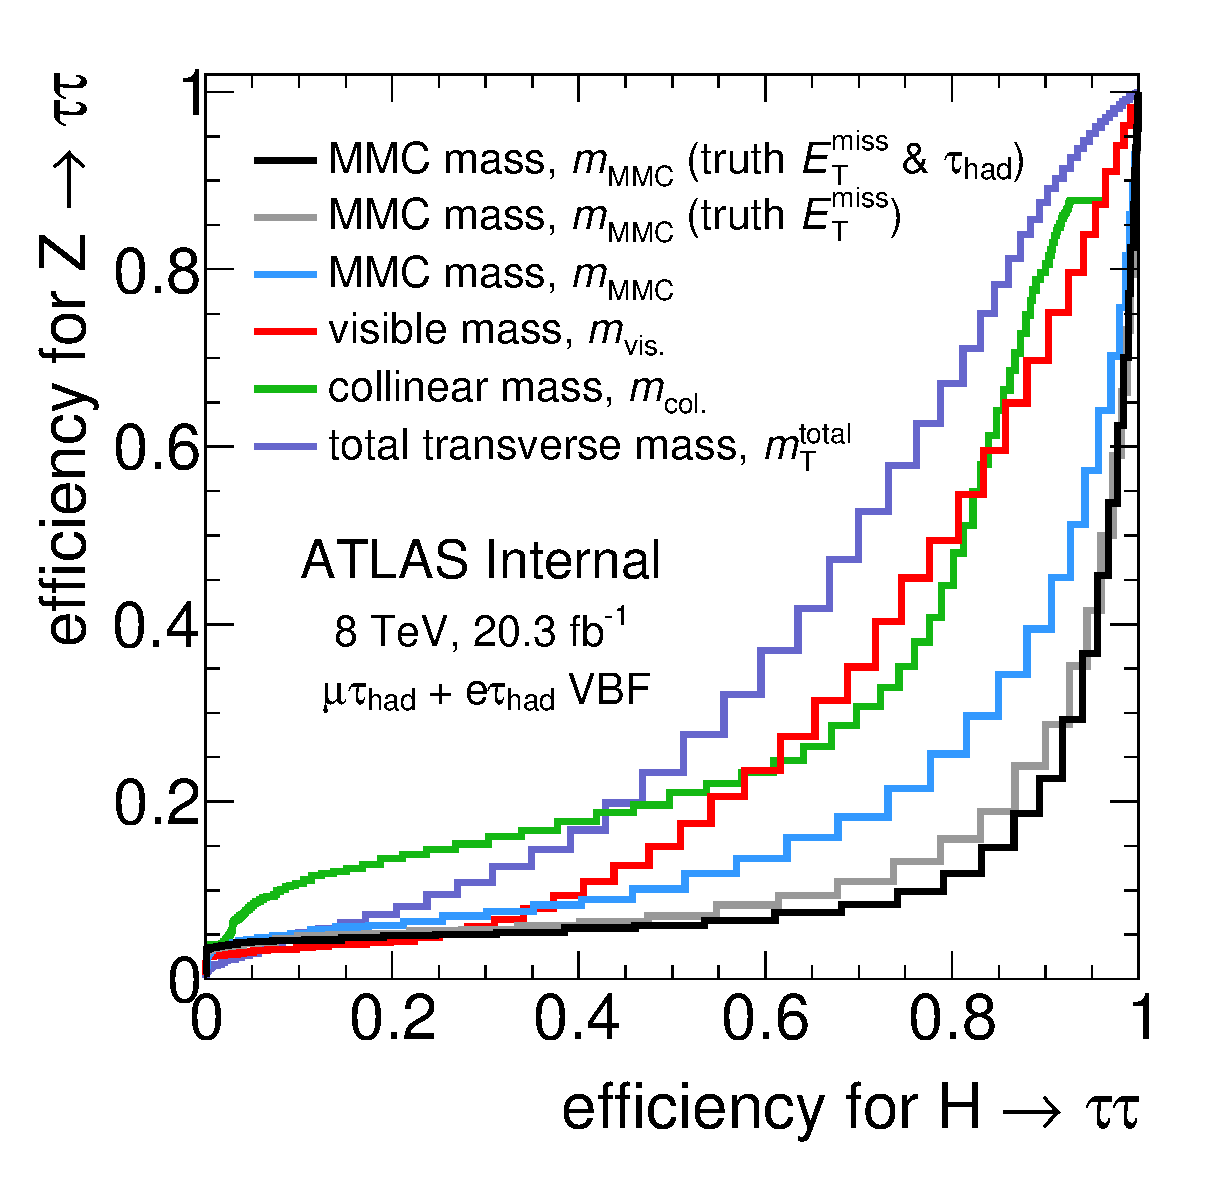
\includegraphics[width=0.48\textwidth]{figures/mtautau/mtautau-ROC-vbf}
  \caption{Variables.}
  \label{fig:strategy-mtautau-ROC}
\end{figure}
% ---------------------------------------------------------------------------------

\section{MVA discrimination}
\label{sec:strategy-mva}

% boost
% ---------------------------------------------------------------------------------
\begin{figure}[tp]
  \centering
  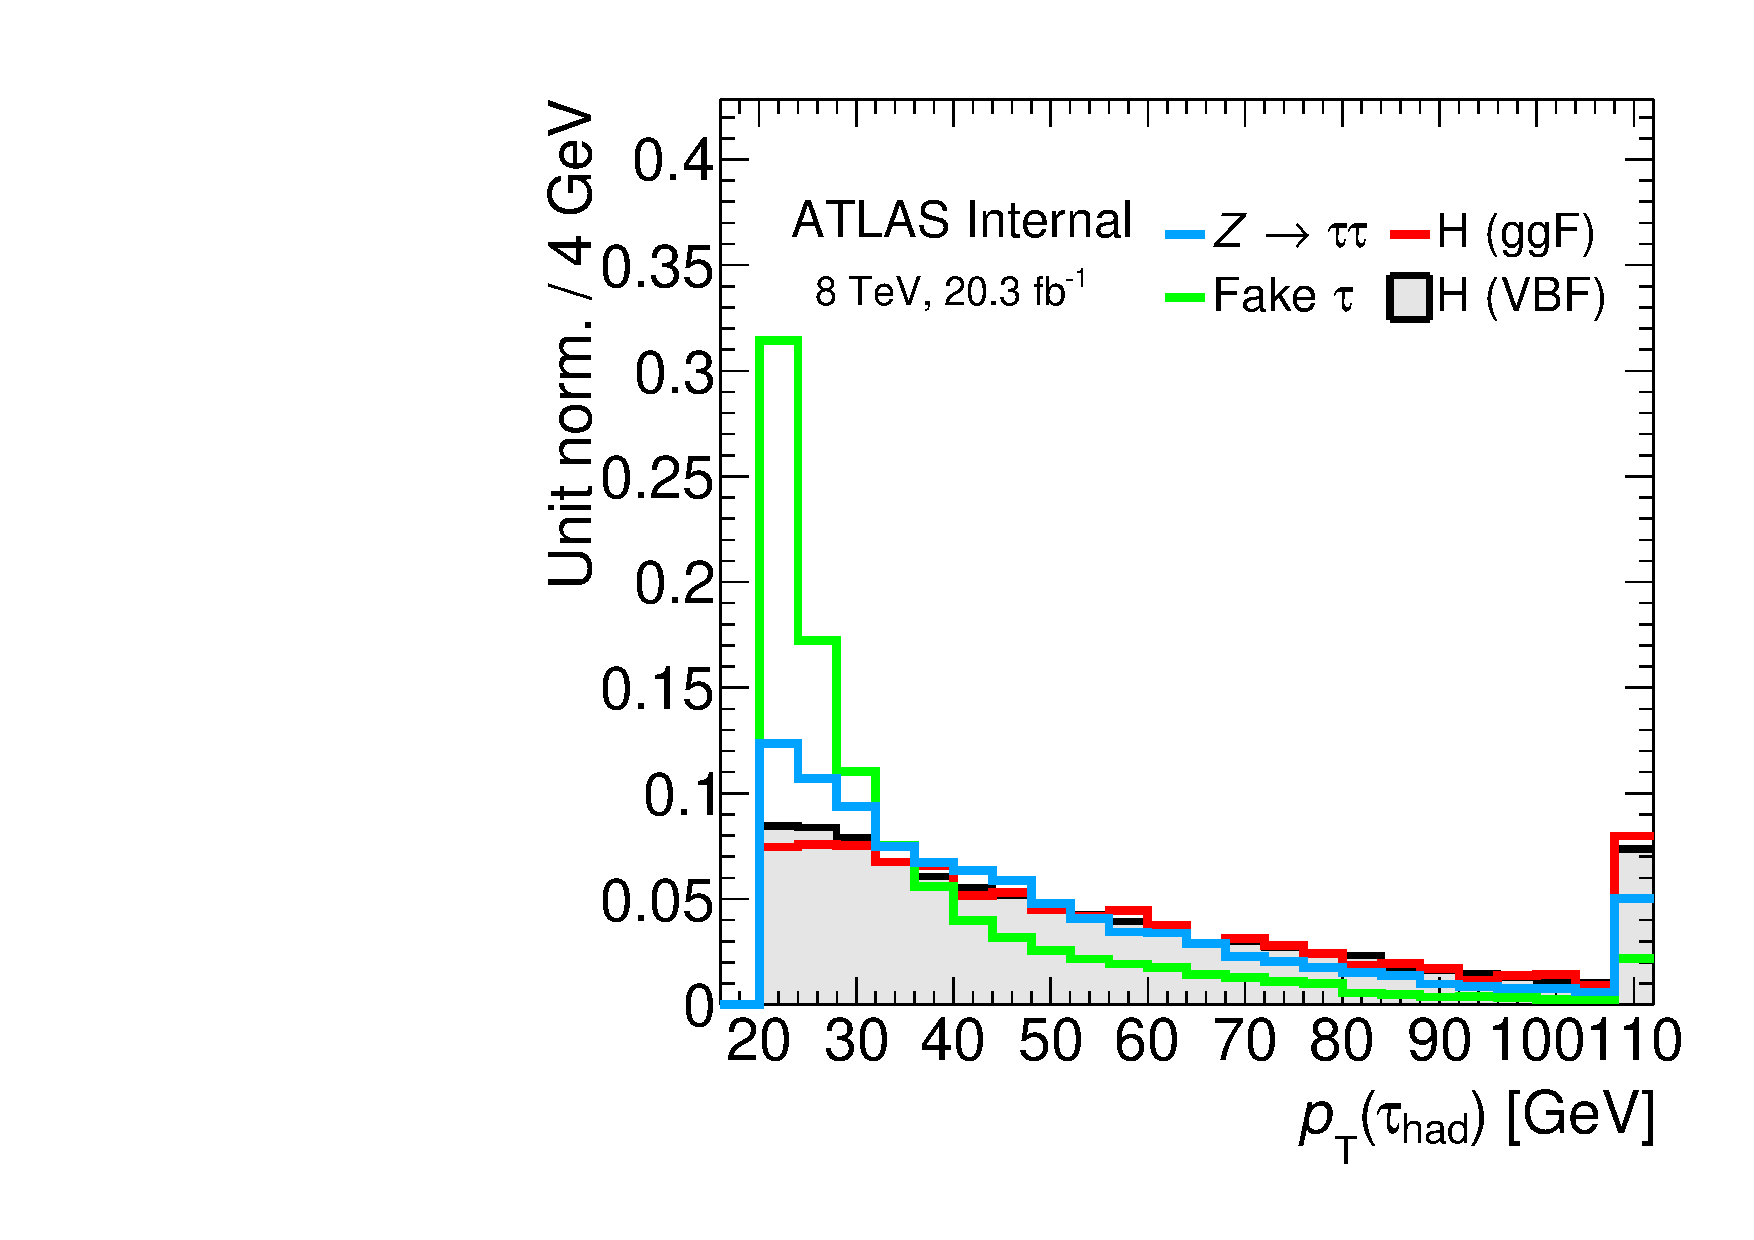
\includegraphics[width=0.35\textwidth]{figures/overlaid/boost/tau-pt}
  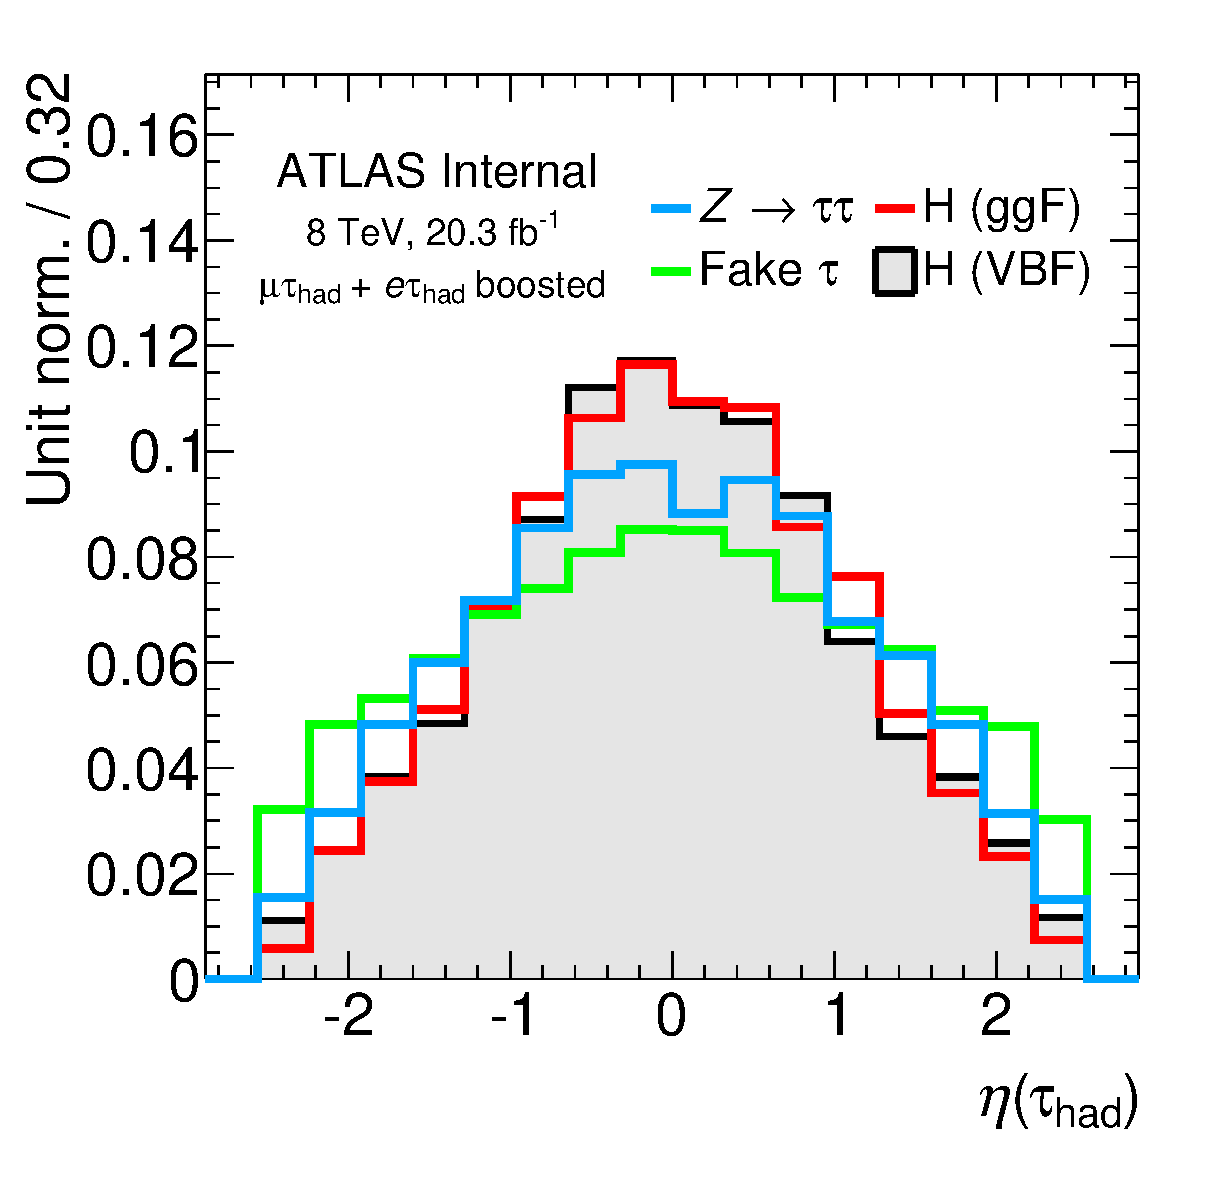
\includegraphics[width=0.35\textwidth]{figures/overlaid/boost/tau-eta}
  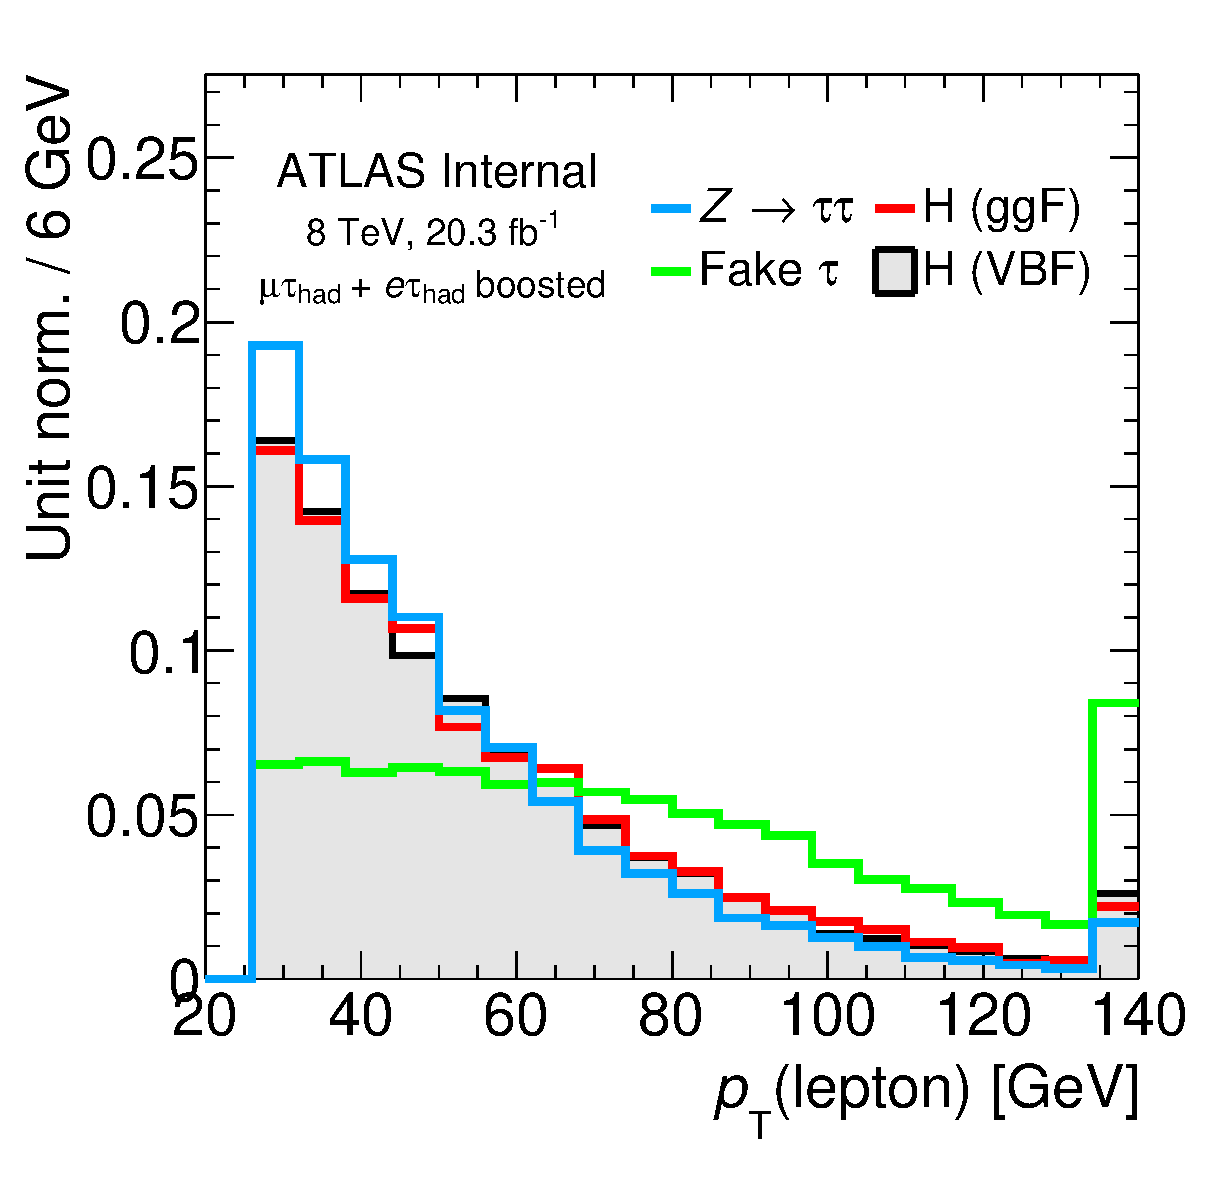
\includegraphics[width=0.35\textwidth]{figures/overlaid/boost/lep-pt-hi}
  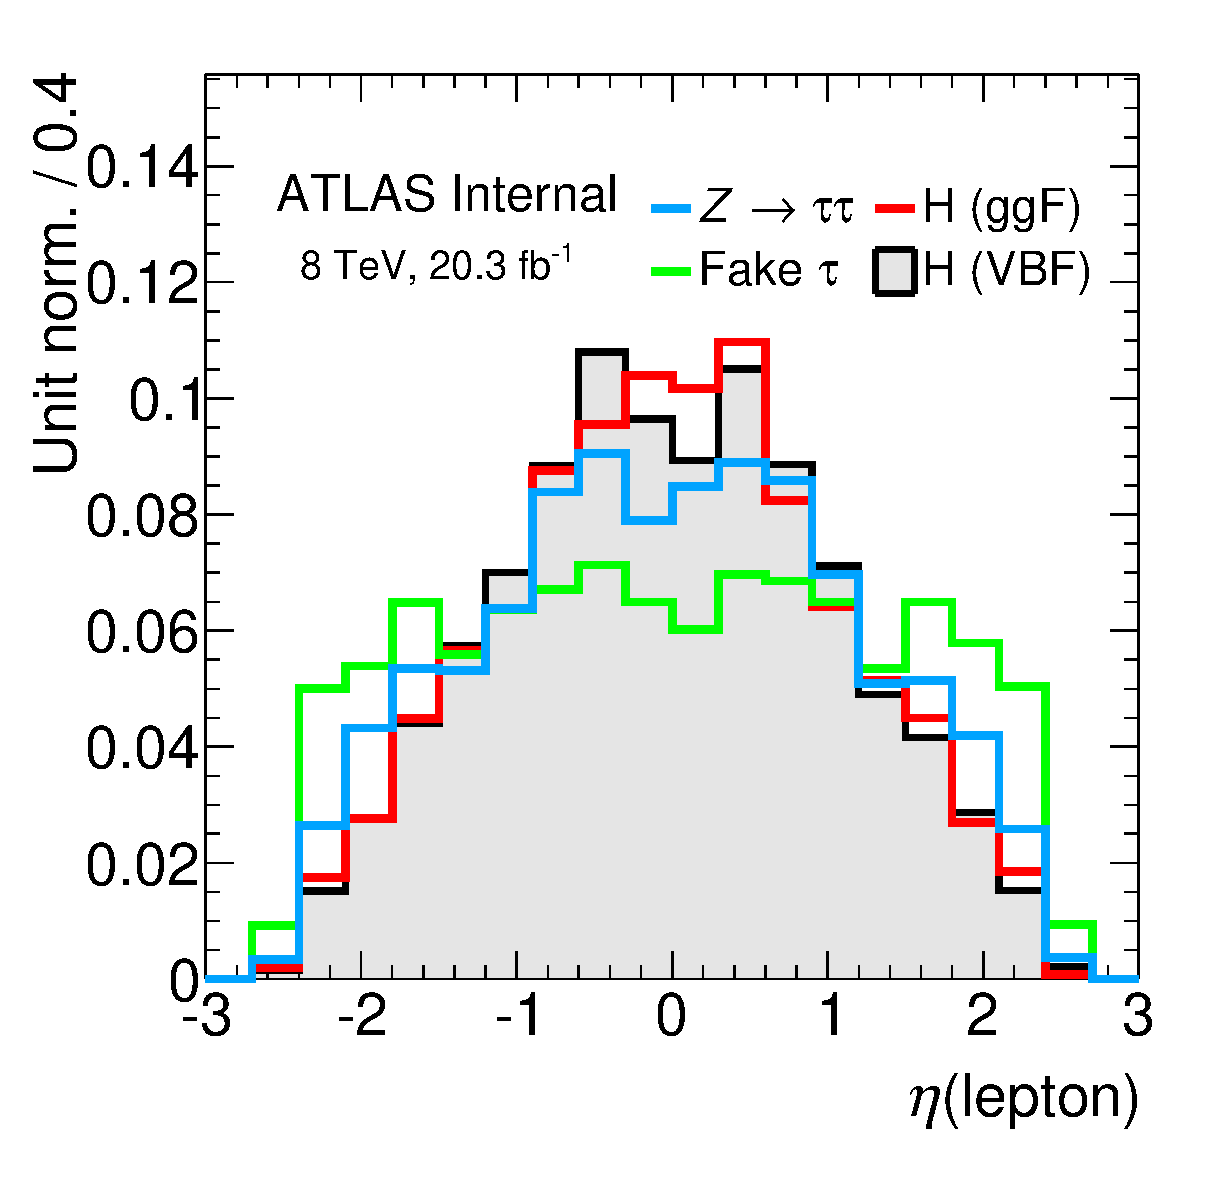
\includegraphics[width=0.35\textwidth]{figures/overlaid/boost/lep-eta}
  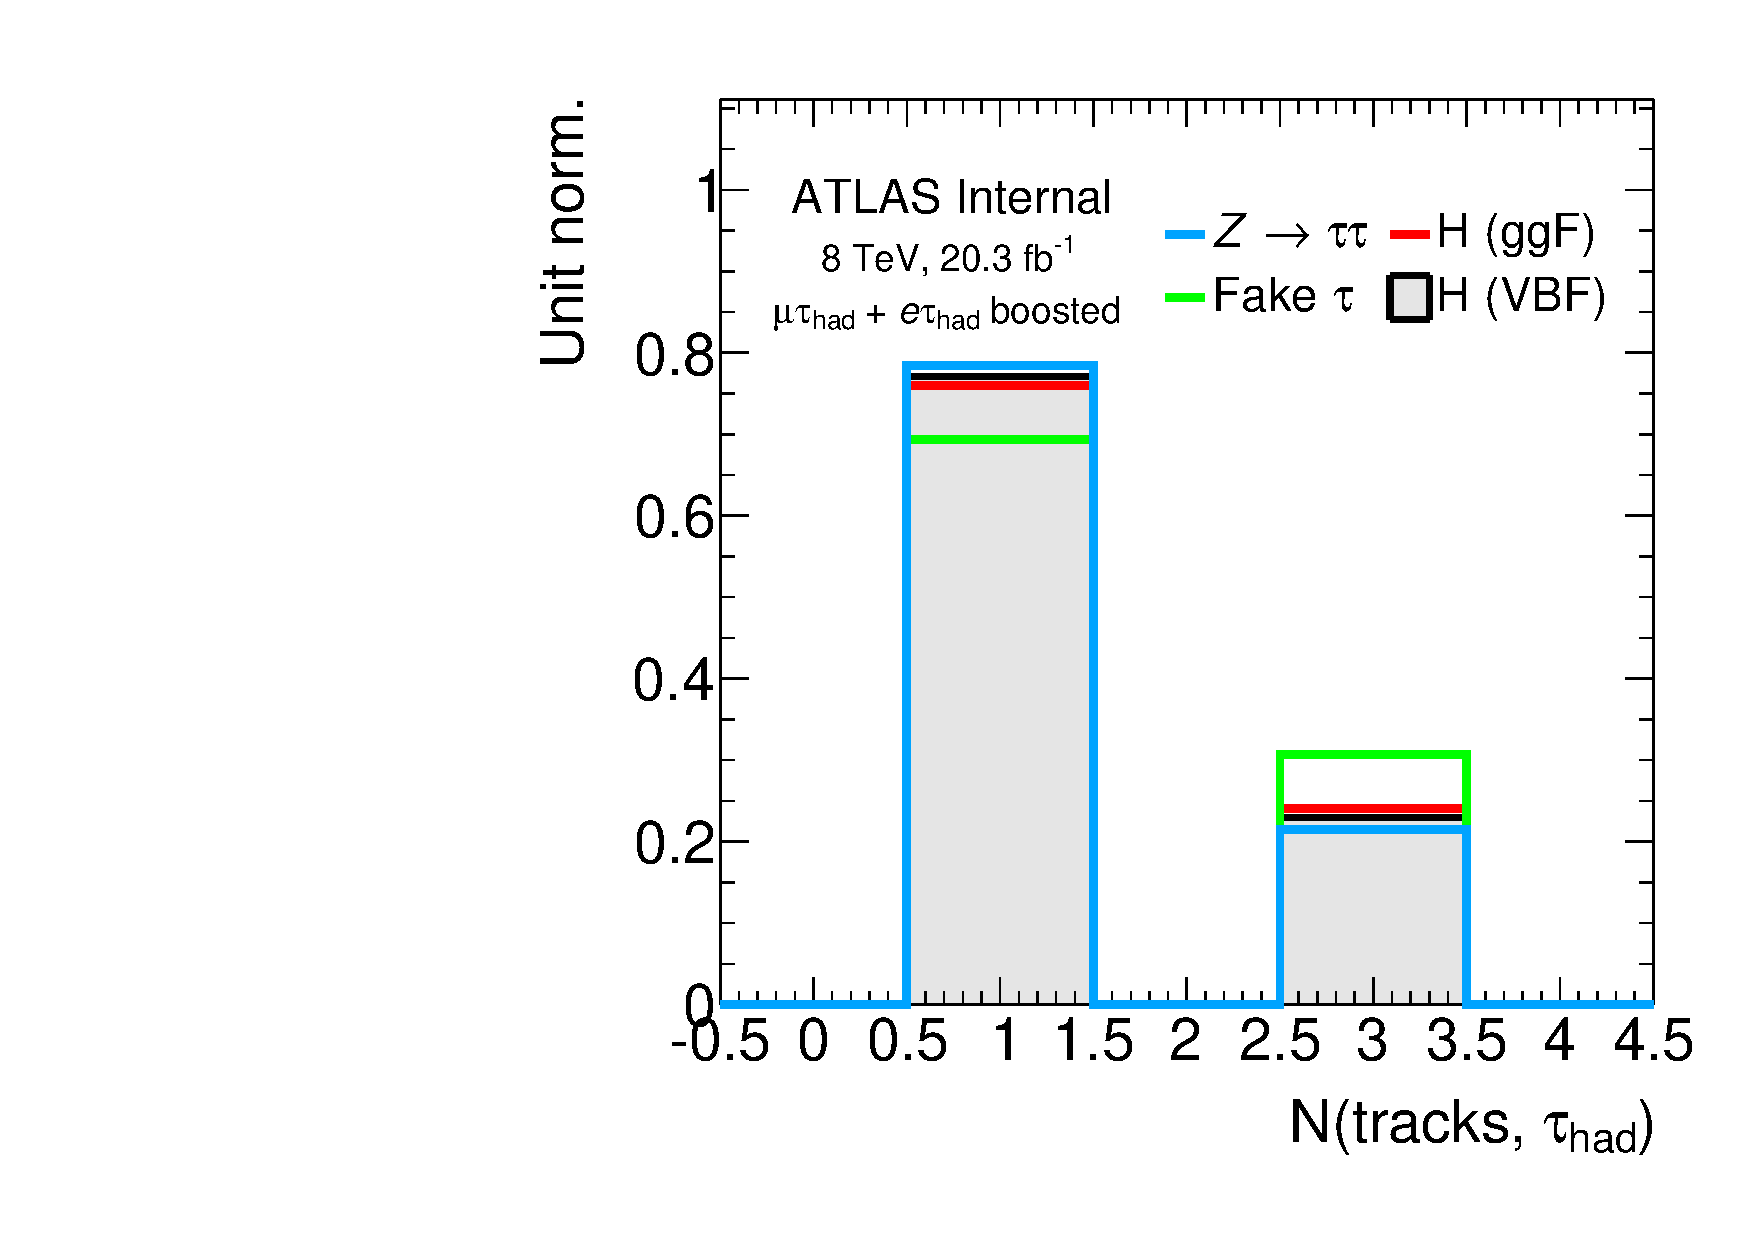
\includegraphics[width=0.35\textwidth]{figures/overlaid/boost/tau-numTrack}
  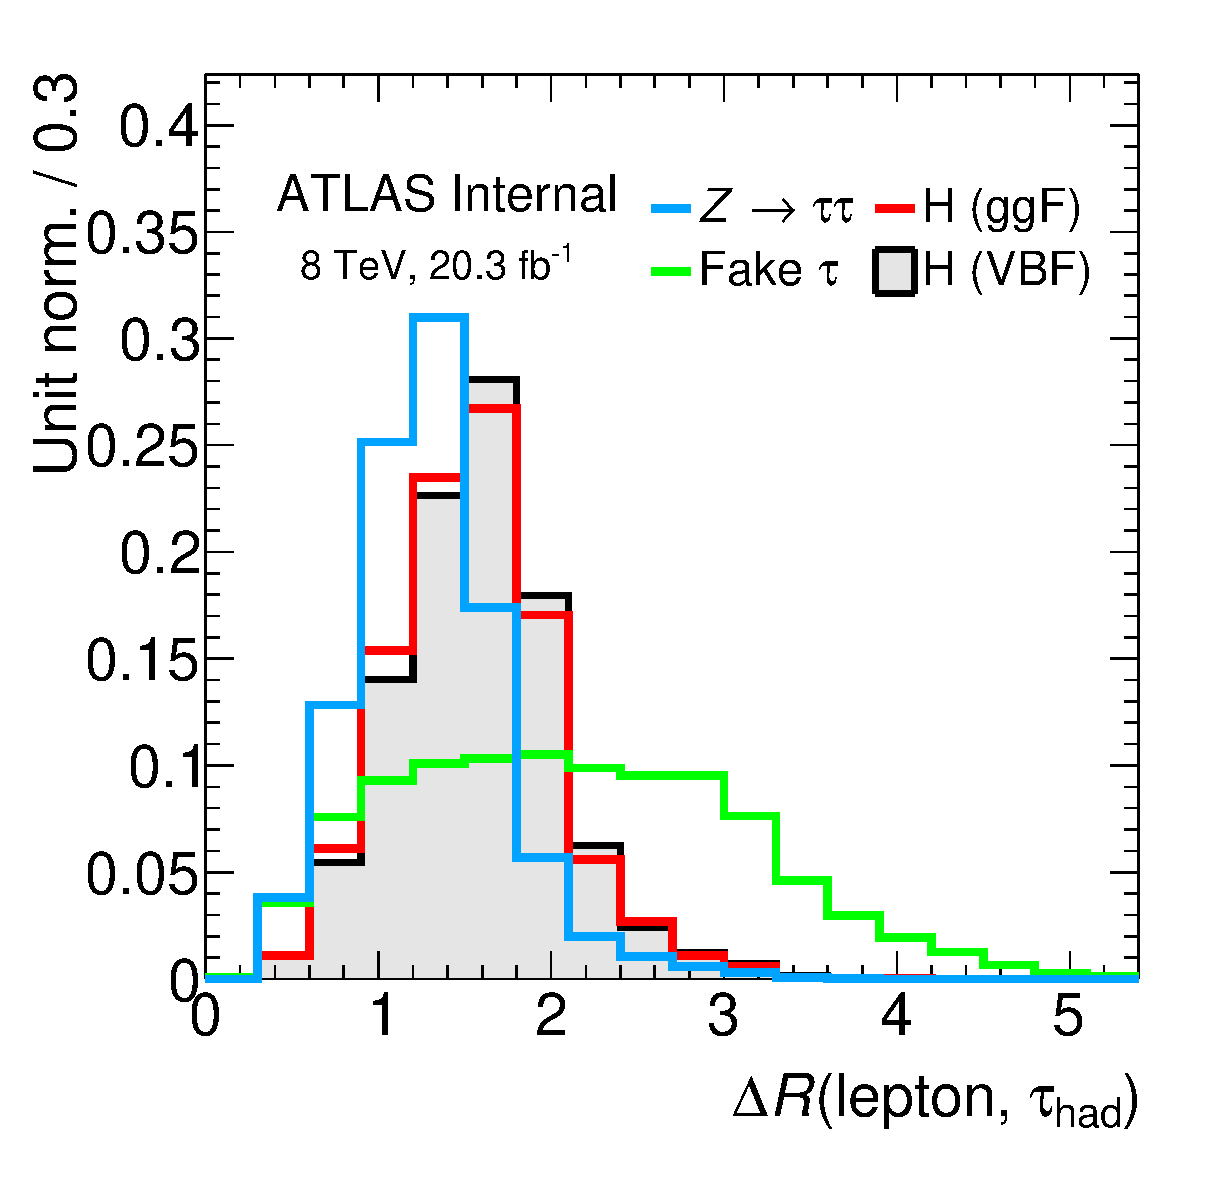
\includegraphics[width=0.35\textwidth]{figures/overlaid/boost/taulep-dR}
  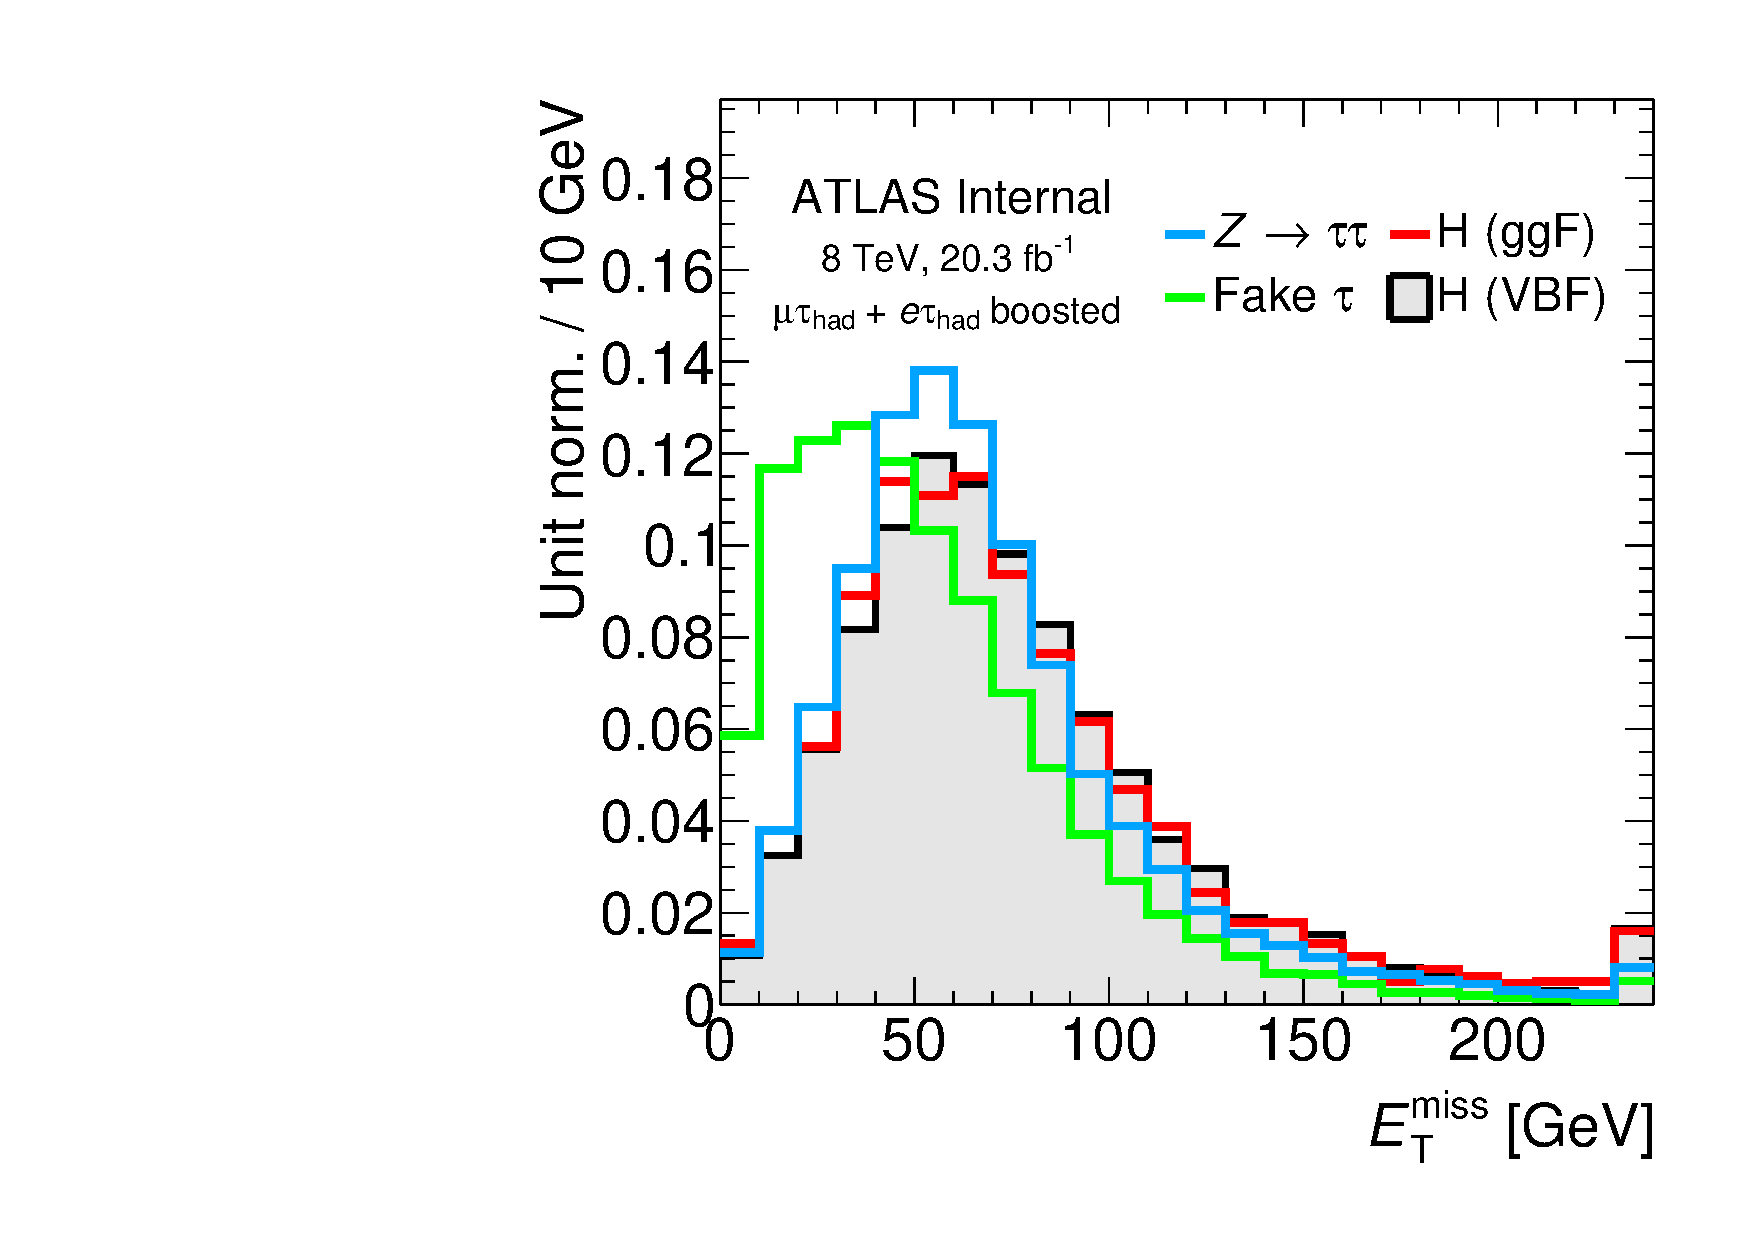
\includegraphics[width=0.35\textwidth]{figures/overlaid/boost/met-pt-hi}
  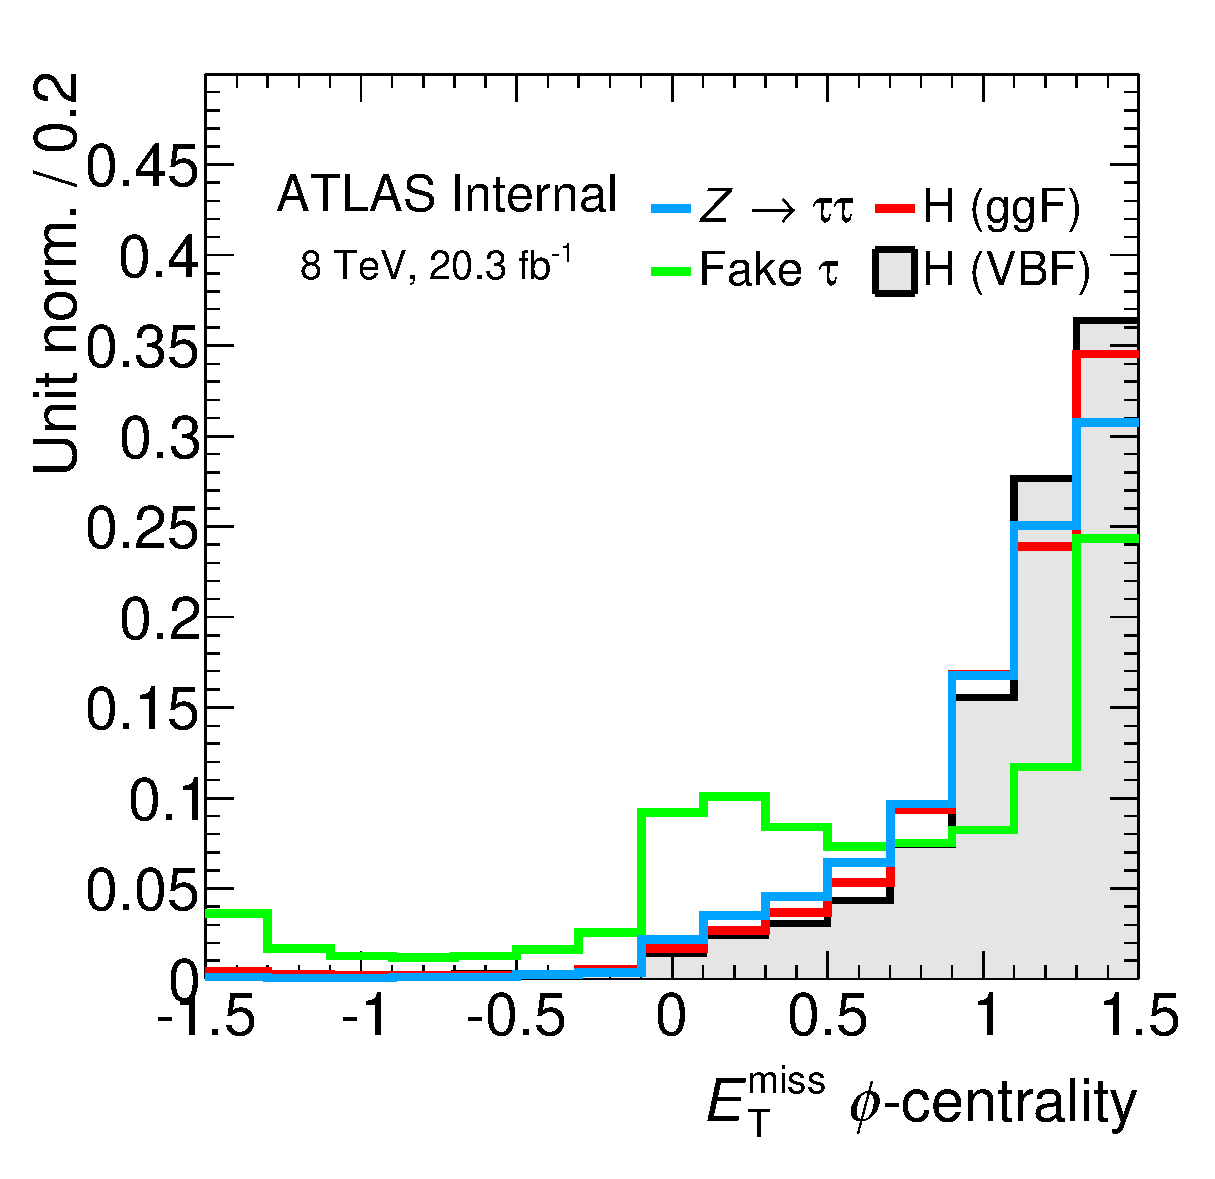
\includegraphics[width=0.35\textwidth]{figures/overlaid/boost/met-phi-centrality}
  \caption{Variables.}
  \label{fig:strategy-overlaid-boost-taus}
\end{figure}
\begin{figure}[tp]
  \centering
  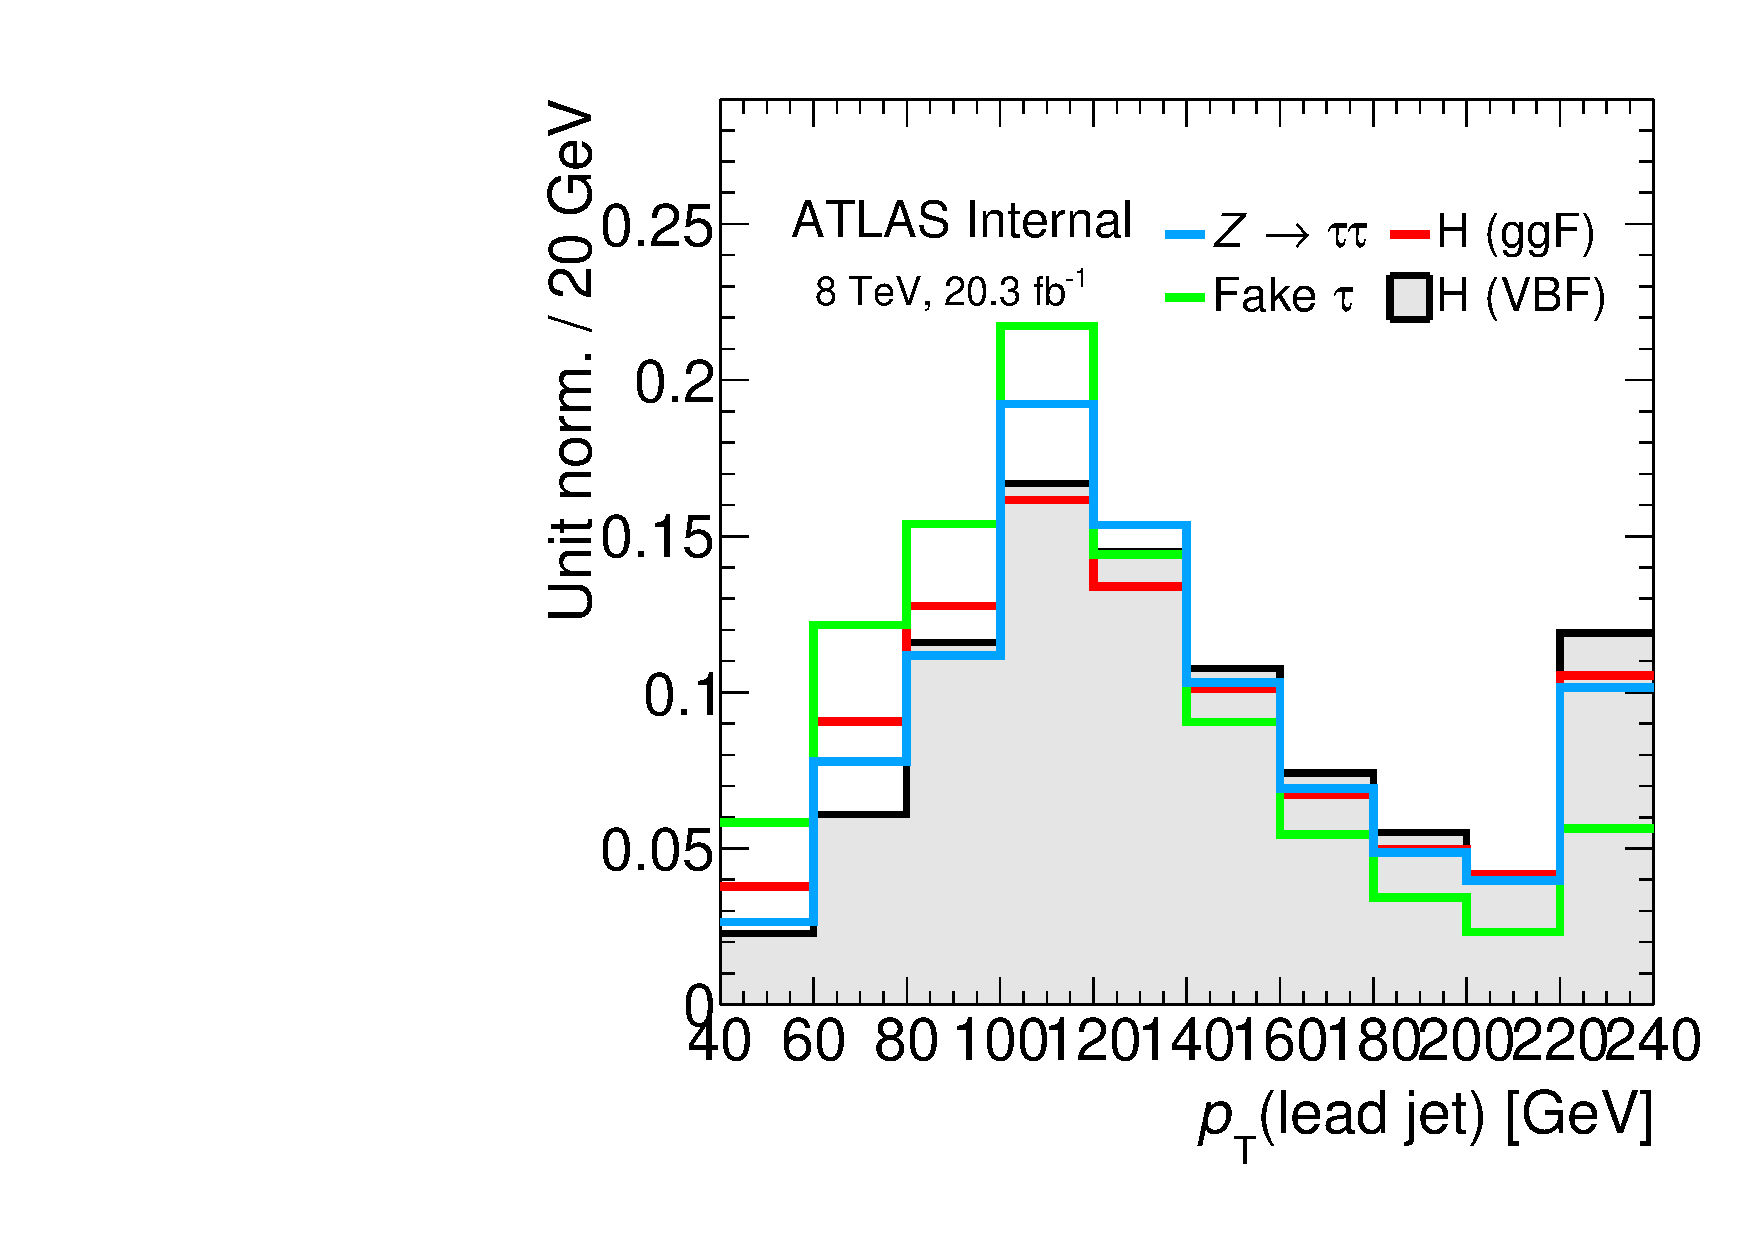
\includegraphics[width=0.45\textwidth]{figures/overlaid/boost/jet-1-pt}
  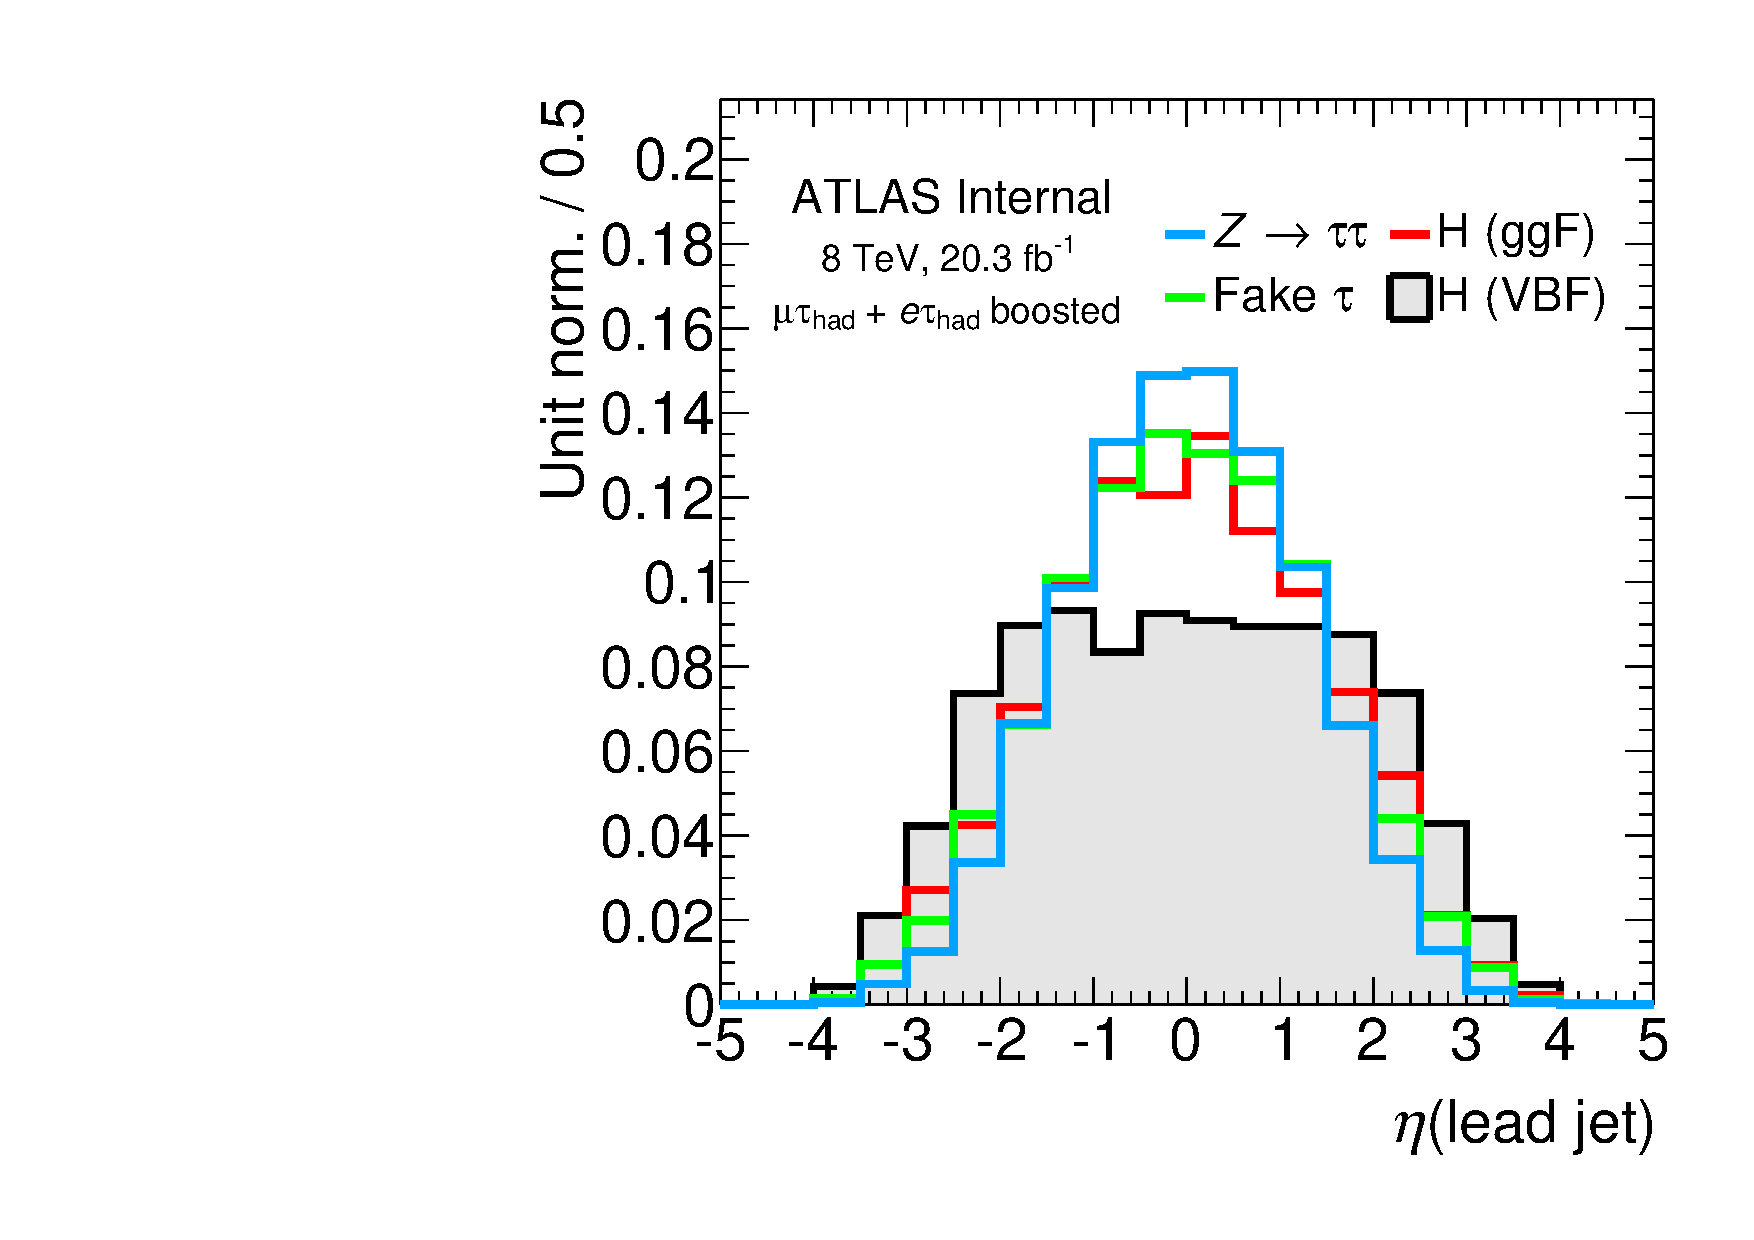
\includegraphics[width=0.45\textwidth]{figures/overlaid/boost/jet-1-eta}
  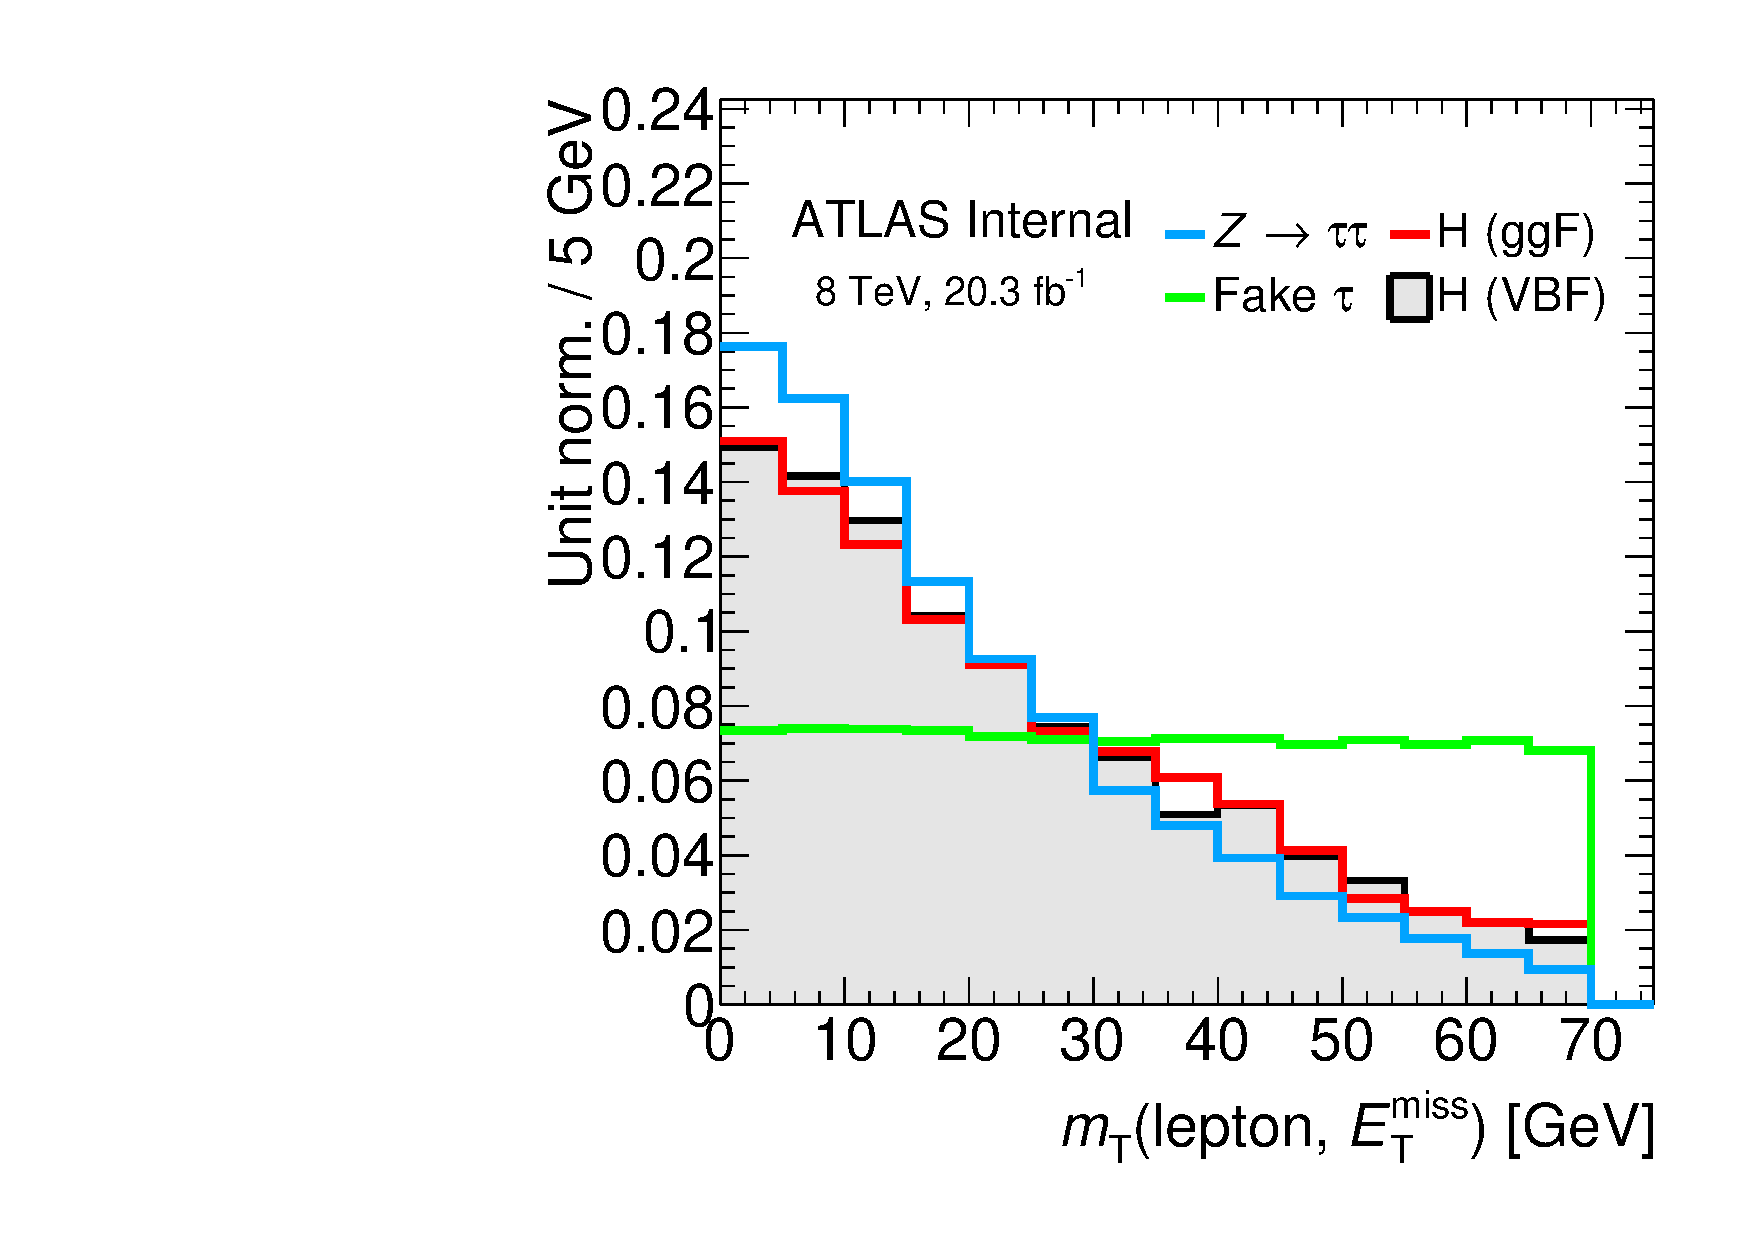
\includegraphics[width=0.45\textwidth]{figures/overlaid/boost/mT}
  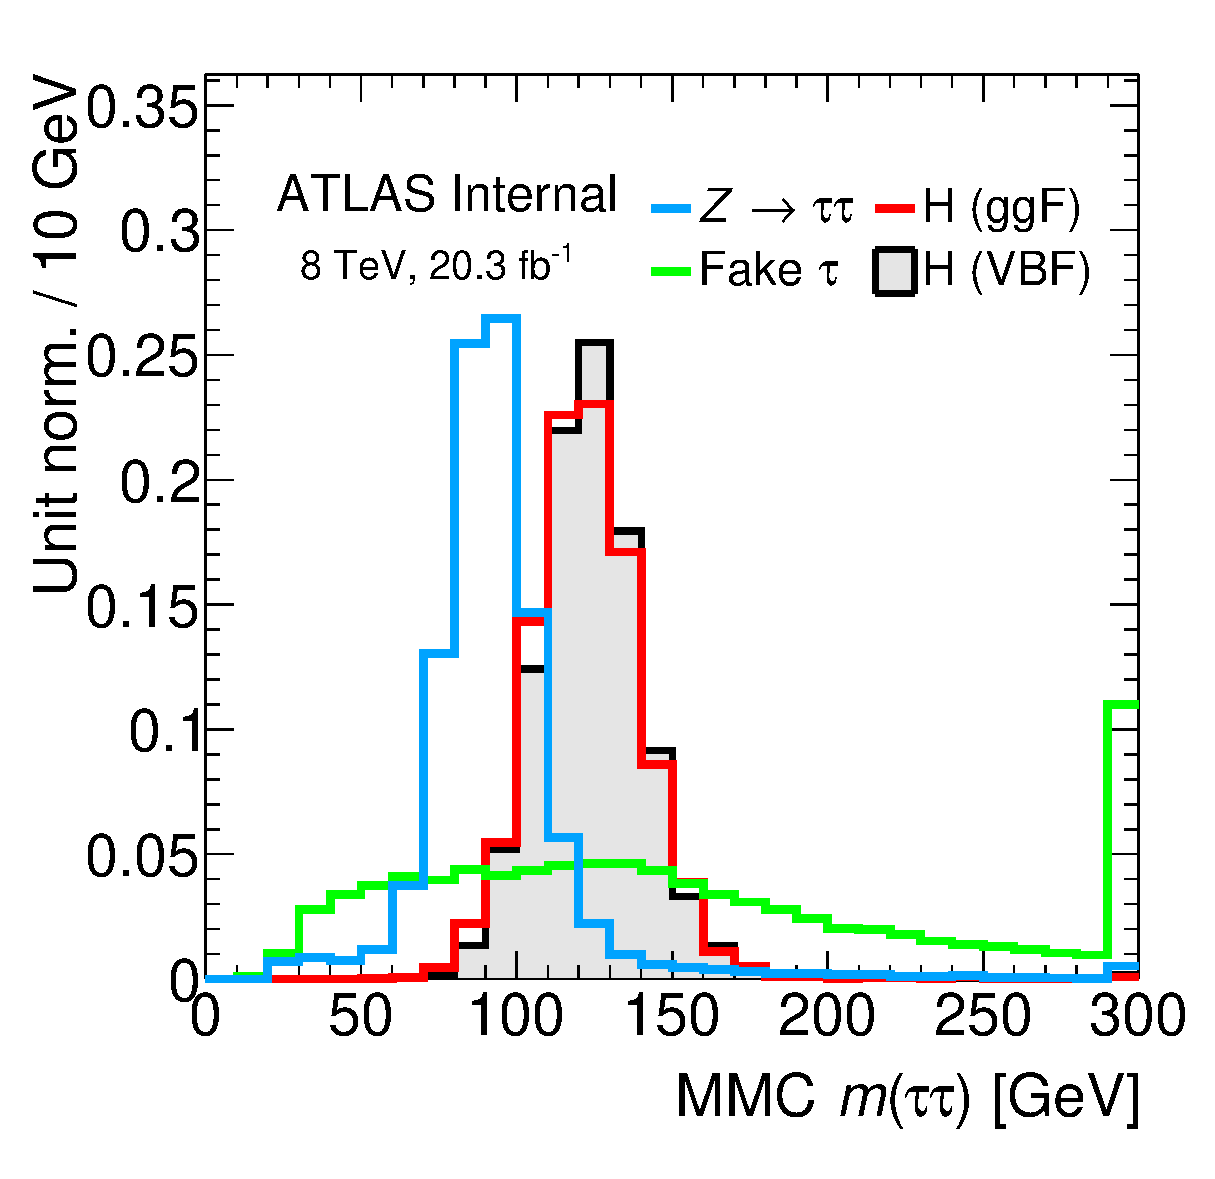
\includegraphics[width=0.45\textwidth]{figures/overlaid/boost/mMMC}
  \includegraphics[width=0.45\textwidth]{figures/overlaid/boost/H-pt-hi}
  \includegraphics[width=0.45\textwidth]{figures/overlaid/boost/BDTEve-boost}
  \caption{Variables.}
  \label{fig:strategy-overlaid-boost-other}
\end{figure}
% ---------------------------------------------------------------------------------

% VBF
% ---------------------------------------------------------------------------------

\begin{figure}[tp]
  \centering
  \includegraphics[width=0.35\textwidth]{figures/overlaid/vbf/tau-pt}
  \includegraphics[width=0.35\textwidth]{figures/overlaid/vbf/tau-eta}
  \includegraphics[width=0.35\textwidth]{figures/overlaid/vbf/lep-pt-hi}
  \includegraphics[width=0.35\textwidth]{figures/overlaid/vbf/lep-eta}
  \includegraphics[width=0.35\textwidth]{figures/overlaid/vbf/tau-numTrack}
  \includegraphics[width=0.35\textwidth]{figures/overlaid/vbf/taulep-dR}
  \includegraphics[width=0.35\textwidth]{figures/overlaid/vbf/met-pt-hi}
  \includegraphics[width=0.35\textwidth]{figures/overlaid/vbf/met-phi-centrality}
  \caption{Variables.}
  \label{fig:strategy-overlaid-vbf-taus}
\end{figure}
\begin{figure}[tp]
  \centering
  \includegraphics[width=0.35\textwidth]{figures/overlaid/vbf/jet-1-pt}
  \includegraphics[width=0.35\textwidth]{figures/overlaid/vbf/jet-1-eta}
  \includegraphics[width=0.35\textwidth]{figures/overlaid/vbf/jet-2-pt}
  \includegraphics[width=0.35\textwidth]{figures/overlaid/vbf/jet-2-eta}
  \includegraphics[width=0.35\textwidth]{figures/overlaid/vbf/dijet-m-veryhigh}
  \includegraphics[width=0.35\textwidth]{figures/overlaid/vbf/jets-deta}
  \includegraphics[width=0.35\textwidth]{figures/overlaid/vbf/jets-dphi}
  \includegraphics[width=0.35\textwidth]{figures/overlaid/vbf/jets-etaprod}
  \caption{Variables.}
  \label{fig:strategy-overlaid-vbf-jets}
\end{figure}
\begin{figure}[tp]
  \centering
  \includegraphics[width=0.45\textwidth]{figures/overlaid/vbf/mT}
  \includegraphics[width=0.45\textwidth]{figures/overlaid/vbf/mMMC}
  \includegraphics[width=0.45\textwidth]{figures/overlaid/vbf/H-pt-hi}
  \includegraphics[width=0.45\textwidth]{figures/overlaid/vbf/system-pt}
  \includegraphics[width=0.45\textwidth]{figures/overlaid/vbf/lep-eta-centrality}
  \includegraphics[width=0.45\textwidth]{figures/overlaid/vbf/BDTEve-VBF}
  \caption{Variables.}
  \label{fig:strategy-overlaid-vbf-other}
\end{figure}
% ---------------------------------------------------------------------------------

% VBF correlations
% ---------------------------------------------------------------------------------
\clearpage
\begin{figure}[tp]
  \centering
  \includegraphics[width=0.98\textwidth]{figures/kinematiccorrelations/mT-vs-mMMC}
  \includegraphics[width=0.98\textwidth]{figures/kinematiccorrelations/taulep_dR-vs-mMMC}
  \caption{Variables.}
  \label{fig:strategy-kinematic-correlations-1}
\end{figure}

\begin{figure}[tp]
  \centering
  \includegraphics[width=0.98\textwidth]{figures/kinematiccorrelations/H_pt-vs-taulep_dR}
  \includegraphics[width=0.98\textwidth]{figures/kinematiccorrelations/met_phi_cent-vs-taulep_dR}
  \caption{Variables.}
  \label{fig:strategy-kinematic-correlations-2}
\end{figure}

\clearpage
\begin{figure}[tp]
  \centering
  \includegraphics[width=0.98\textwidth]{figures/kinematiccorrelations/jj_mass-vs-jj_deta}
  \includegraphics[width=0.98\textwidth]{figures/kinematiccorrelations/jj_mass-vs-jj_etaprod}
  \caption{Variables.}
  \label{fig:strategy-kinematic-correlations-3}
\end{figure}

\begin{figure}[tp]
  \centering
  \includegraphics[width=0.98\textwidth]{figures/kinematiccorrelations/jj_mass-vs-mMMC}
  \includegraphics[width=0.98\textwidth]{figures/kinematiccorrelations/jj_mass-vs-taulep_dR}
  \caption{Variables.}
  \label{fig:strategy-kinematic-correlations-4}
\end{figure}

Here is a citation~\cite{1999.ATLAS.Physics-TDR}.


